\documentclass[11pt]{article}  % include bezier curves
\renewcommand\baselinestretch{1.0}           % single space

\oddsidemargin -10 true pt      % Left margin on odd-numbered pages.
\evensidemargin 10 true pt      % Left margin on even-numbered pages.
\marginparwidth 1.5 true in    % Width of marginal notes.
\oddsidemargin  0 true in       % Note that \oddsidemargin=\evensidemargin
\evensidemargin 0 true in
\topmargin -0.5 true in        % Nominal distance from top of page to top of
\textheight 9.0 true in         % Height of text (including footnotes and figures)
\textwidth 6.5 true in        % Width of text line.
\parindent=0pt                  % Do not indent paragraphs
\parskip=0.15 true in
%\usepackage{color}              % Need the color package
\usepackage{hyperref}
\usepackage[pdftex]{color, graphicx}
%\usepackage{graphicx} %for epsfig
\usepackage{setspace}
\usepackage{graphics}
\usepackage{subfig}
\usepackage{epsfig}
\usepackage{latexsym}
\usepackage{mathrsfs}
\usepackage{eufrak}
\usepackage{amsmath}
\usepackage{graphicx}
\usepackage{longtable}
\usepackage{afterpage}
\usepackage{pdfpages}
\usepackage{tikz}
\usetikzlibrary{decorations.pathmorphing}
\usetikzlibrary{arrows}
\usetikzlibrary{shapes.geometric}
\title{SCOREC libraries for M3D-$C^1$}
\author{Kaushik Kalyanaraman, E. Seegyoung Seol, Mark S. Shephard \\
Past contributor: Fan Zhang} 
\begin{document} 
\maketitle
\tableofcontents

%+++++++++++++++++++++++++++++++++++++++++++++++++++++
\section{Introduction} \label{sec:intro}
%+++++++++++++++++++++++++++++++++++++++++++++++++++++
%This document overviews the current status of the software that SCOREC provides to M3D-C1 \cite{jardin2004triangular,jardin2007high,ferraro2009calculations,jardin2012review,jardin2012multiple, Ferraro2011, Ferraro2014} and the requirements of the new capability that enables M3D-C1 to switch between  modes. M3D-C1  applies C$^1$  4$^{th}$ order element to solve the magnetohydrodynamics (MHD) equations and simulates the nonlinear instability of the plasma in the tokamak.  The case of non-axis-symmetric instability requires the simulation to be performed on the 3D mesh.  The new  capability  to be developed will allow  M3D-$C^1$  to start with a 2D analysis and switch to 3D when a full 3D discretization is needed. 
%MHD is the macroscopic description of plasmas as the electrically conducting fluids \cite{goedbloed2004principles}.  The birth of MHD dates back to 1940s by the discoveries of Hannes Alfv{\'e}n \cite{alfven1942existence,alfven1950cosmical}. MHD have been widely applied as the theoretical tool in the areas ranging from fundamental scientific studies on the astrophysics and cosmology to engineering applications such as  the fusion power generation in tokamaks since then. 

Tokamak fusion reactors \cite{wesson2011tokamaks} are the experimental approach to study magnetically confined sustainable fusion reactions. The basic tokamak is a torus that is symmetric along the toroidal direction. The fusion material exists as the state of plasma and is confined by the magnetic field \cite{chen1984introduction} in the torus. M3D-$C^1$ ~\cite{jardin2004triangular,jardin2007high,ferraro2009calculations,jardin2012review,jardin2012multiple, Ferraro2011, Ferraro2014} is a fusion plasma simulation code under development at PPPL.  It studies non-linear instabilities of plasmas in the tokamak.  C$^1$ finite elements are applied by M3D-$C^1$ to solve fourth order PDEs derived from the magnetohydrodynamics (MHD) equations. 

This document overviews the development status of integrating M3D-$C^1$ and SCOREC tools to provide a parallel adaptive loop that can adapt both the mesh and the level of the discretization in the toroidal direction of the tokamak.

M3D-$C^1$ perform three types of simulations \cite{Jardin2014Extend}. 
\begin{itemize}
\item The 3D nonlinear simulation uses the $C^1$ wedge element \cite{jardin2012multiple} and the PDEs are discretized in full 3D.  
\item The 2D nonlinear (3D axis-symmetric) simulation assumes the solution is symmetric in the toroidal direction ($\partial/\partial \varphi =0$) and it uses the $C^1$ reduced quintic triangle element  \cite{jardin2004triangular} that the PDEs are discretized only on the tokamak cross section~\cite{wesson2011tokamaks,stacey1982fusion}. 
\item The 3D linear (3D analytic) simulation assumes the fields in the toroidal direction vary as $\sim e^{i\cdot n\varphi}$. It applies the $C^1$ triangle element to discretize the PDEs on the tokamak cross section and  the complex arithmetic is used.
\end{itemize}

A parallel adaptive loop that couples the three types of simulations needs to be developed. The loop starts with the 2D nonlinear simulation and  axis-symmetric instabilities are developed on the tokamak cross section.  The 3D linear simulation is used periodically to check  whether the eigen-modes in the toroidal direction are stable. The simulation is switched to the 3D nonlinear if instabilities both on the cross section and in the toroidal direction of the tokamak need to developed.  The 3D nonlinear simulation represents a full set of instabilities in all the spacial directions of the tokamak.

The document is organized as the following. Section \ref{sec:general} discusses the  components of a general mesh-based adaptive analysis. Section \ref{sec:m3dc1} discusses the  workflow of M3D-$C^1$. The set of MHD equations solved  in M3D-$C^1$ is presented in Section \ref{sec:mhd} . The geometric model and mesh aspects are discussed in Section \ref{sec:domain}. Section  \ref{sec:m3dc1_dis} introduces the discretization methods applied in M3D-$C^1$.  The global discrete system formation and solve are discussed in Section \ref{sec:form-eq} focusing on the usage of PETSc. Section \ref{sec:impl} discusses the data structure and algorithm aspects to support the  extended adaptive loop under development that couples different types of simulations in M3D-$C^1$.  Section \ref{sec:issues} discusses the S/W issues involved in the development.  

%+++++++++++++++++++++++++++++++++++++++++++++++++++++
\section{Mesh-based Adaptive Analysis} \label{sec:general}
%+++++++++++++++++++++++++++++++++++++++++++++++++++++

Mesh-based methods such as the finite element and the finite volume methods are used to solve the PDEs numerically.  The reliability  of simulation results is efficiently improved through the adaptive mesh control \cite{shephardmethods}. A mesh-based adaptive analysis program generally includes the following components (Figure \ref{fig:femstructure}).
\begin{enumerate}
\item[(A)] A mathematical model defined by PDEs that represents the governing equations of problems studied by the analysis program.
\item[(B)] A mesh infrastructure that provides the interface to the geometric model of the computational domain and manages the mesh.
\item[(C)] A component to discretize the PDEs over mesh entities. Given the inputs of geometric domain, mesh, and the input field information describing the distribution of the material properties, the solutions from previous load step, and/or the exterior load, it outputs the element contributions to the discrete equation. 
\item [(D)] A component to assemble the discrete equation. Given the element contributions and  the ordering of the degrees of the freedom (DOFs), it assembles the global discrete equation.
\item[(E)] A component to solve global discrete equation. It outputs the solution fields.
\item[(F)] A component of solution assessment. Given the solution field, it assesses the solution quality and generates the correction indication field.
\item[(G)] A component to improve the mesh and map the fields. Given the correction indication field, the mesh is improved adaptively and the solution fields are mapped from the original mesh to the improved mesh.
\end{enumerate}

\begin{figure}[hbt]
\center

\includegraphics[width=5.5in]{fig/FEMStructure.png}
\caption{\small{The components of mesh-based adaptive analysis}} 
\label{fig:femstructure}
\end{figure}

%+++++++++++++++++++++++++++++++++++++++++++++++++++++
\subsection{Mesh Infrastructure}
%+++++++++++++++++++++++++++++++++++++++++++++++++++++
The mesh infrastructure (B in Figure \ref{fig:femstructure}) provides the interface to the geometric model of the computational domain and manages the evolving mesh representation. The geometric model is defined in terms of the abstraction of the topological entities and their adjacencies \cite{weiler1986topo}. The information that defines the shape of the model entities is associated with the topological entities. The mesh is managed by the infrastructure for adaptive simulations on massively parallel computers (see \cite{Seol2014} for the general discussion of the mesh infrastructure). 

%+++++++++++++++++++++++++++++++++++++++++++++++++++++
\subsection{Field}
%+++++++++++++++++++++++++++++++++++++++++++++++++++++
A field describes the variation or distribution of tensor quantities in the governing equations over the geometric domain (see the information flow in Figure \ref{fig:femstructure}). The spatial variation of the field on the mesh is defined in terms of polynomial functions defined over the mesh entities. 
Define $N_i$ as the shape function associated with the mesh entity and $\lambda_i$ as the multiplier of the shape function. A field distribution on the mesh, $\mathbf{f}$, can be written as
\begin{equation}
\mathbf{f}=\sum_i\mathbf{\lambda}_iN_i,
\end{equation}

The field $\mathbf{f}$ can be a tensor which will be expanded into the appropriated number of scalar components. Typically the same shape functions are used for each component. 

The following information is needed to create a field on a mesh.
\begin{itemize}
\item The mesh that provides the spacial discretization of the geometric domain. 
\item The definition of the shape function associated with the mesh entity.  The shape function is generally defined  as piece-wise polynomials that satisfy a specific continuity requirement such as continuous Lagrange, discontinuous Lagrange, Hermitian functions, splines, etc.
\item The number of scalar components in the field tensor. The number of components depends on the dimension of the problem, and the order and symmetry of the tensor. For example, the number of scalars associated with the tensor in the three dimensional space decomposed into Cartesian components is  1, 3, 6, and 9  for the field with the type as scalar, vector, symmetric and asymmetric $2^{nd}$-order respectively. 
\end{itemize}

When the multipliers are DOFs, they are ordered such that an integer equation number is assigned to each DOF to build the matrices and vectors in the global discrete system for the analysis program. 

%+++++++++++++++++++++++++++++++++++++++++++++++++++++
\subsection{Global Discrete Equation Solver}
%+++++++++++++++++++++++++++++++++++++++++++++++++++++

The global discrete equation is assembled and solved to obtain the solution field (D and E in Figure \ref{fig:femstructure}). The global discrete equation takes the form as
\begin{equation}
S \mathbf{u}^{n+1} = D \mathbf{u}^n +\mathbf{f}, \label{eqn:sys}
\end{equation}
where $S$ and $D$ are matrices assembled from the element contributions, $\mathbf{u}^{n+1}$ and $\mathbf{u}^{n}$ are solution vectors at step $n+1$ and $n$ respectively, and $\mathbf{f}$ is a vector assembled from the element contributions. 


%+++++++++++++++++++++++++++++++++++++++++++++++++++++
\section{M3D-$C^1$ Adaptive Loop}\label{sec:m3dc1}
%+++++++++++++++++++++++++++++++++++++++++++++++++++++
\begin{figure}[hbt]
\center

\includegraphics[width=5.5in]{fig/M3DC1Loop.png}
\caption{\small{The loop on the 2D mesh}}
\label{fig:M3DC1Loop}
\end{figure}

Figure \ref{fig:M3DC1Loop} illustrates the workflow of adaptive loops for M3D-$C^1$ which includes the following. \textit{\textcolor{blue}{Mark: relate back by saying it is Figure 1 indicating specific software component being used.}}

\begin{itemize}
\item{[A in Figure \ref{fig:M3DC1Loop}]} Section \ref{sec:mhd} discusses the mathematical model of M3D-$C^1$.
\item{[B in Figure \ref{fig:M3DC1Loop}]} A geometric model and distributed mesh are loaded in the parallel unstructured mesh management infrastructure (PUMI) \cite{pumi-web-page, Seol2014}. PUMI provides the interface to the geometric model of the tokamak and manages the distributed mesh. 
  \begin{itemize}
  \item In 2D, a 2D mesh on the toroidal plane is generated with Simmetrix mesh generation tool \cite{simmetrix-web-page}
  \item In 3D, processes are grouped and each process group loads the same distributed 2D mesh. Then 3D mesh is constructed in the PUMI.
  \end{itemize}
Section \label{sec:domain} presents the geometric model and mesh for M3D-$C^1$.

\item{[C in Figure \ref{fig:M3DC1Loop}]} The $4^{th}$ order PDEs derived from MHD equations are discretized with the C$^1$  triangle (resp. wedge) element in 2D (resp. 3D) \cite{jardin2004triangular,ferraro2009calculations, jardin2012multiple} and the element contributions to the stiffness matrix and the force vector are calculated.  The geometric entity that a mesh entity is classified on identifies the set of the governing equation applied in a specific type of the region such as the plasma, the material wall or the vacuum. The geometric shape information such as the normal direction and curvature provides the necessary boundary information during the  PDE discretization process \cite{jardin2010computational}. The input fields needed to define the element contributions include the axis-symmetric static equilibrium of the ideal MHD and/or the solution field from the previous time step. Section \ref{sec:m3dc1_dis} discusses the details of PDE discretization for M3D-$C^1$.
\item{[D in Figure \ref{fig:M3DC1Loop}]} The element contributions to the stiffness matrix and the force vector are assembled to form the global discrete equation. A global DOF ordering that assigns integer labels to DOFs associated with the mesh vertex is calculated. The integer corresponds to the equation number in the global discrete system. Section \ref{sec:form-eq} presents the details of forming stiffness matrix and the force vector for M3D-$C^1$.
\item{[E in Figure \ref{fig:M3DC1Loop}]} The global discrete system is solved to get the solution fields (for instance, velocity and magnetic field) at the current time step. For 2D, SuperLu \cite{superlu_ug99} is used and in 3D, the linear equation solvers in PETSc \cite{petsc-web-page} are used. Section \ref{sec:form-eq} discusses how PETSc is used in M3D-$C^1$.
\item{[F in Figure \ref{fig:M3DC1Loop}]} A mesh size field is defined from the toroidal magnetic flux field  if the mesh on the cross section needs to be improved. 
\item{[G in Figure \ref{fig:M3DC1Loop}]} The mesh is adapted through MeshAdapt \cite{li20053d,sahni2007automated, lu2013parallel}.  The fields on the old mesh are tracked and mapped to a new adapted mesh. 
\end{itemize}


%+++++++++++++++++++++++++++++++++++++++++++++++++++++
\section{Mathematical Model of M3D-$C^1$} \label{sec:mhd}
%+++++++++++++++++++++++++++++++++++++++++++++++++++++
M3D-$C^1$ solves two-fluid MHD equations with $C^1$ finite elements. The governing equations combine the Navier-Stokes equations of fluid dynamics and Maxwell's equations of electromagnetism.  The two-fluid interactions between irons and electrons are included. The set of equations are the following~\cite{ferraro2009calculations, Jardin2013NSTX, Jardin2014Extend, jardin2012multiple}.

\begin{subequations}  \label{eqn:mhd}
\begin{eqnarray}
\frac{\partial n}{\partial t} + \nabla \cdot (n\mathbf{V}) &=&0 \\
nM_i\left(\frac{\partial \mathbf{V}}{ \partial t} + \mathbf{V} \cdot \nabla \mathbf{V}\right) + \nabla p&=&  \mathbf{J} \times \mathbf{B} - \nabla \cdot \mathbf{\Pi}_{GV} - \nabla \cdot \mathbf{\Pi}_{\mu} \\ \label{eqn:velocity}
\frac{\partial \mathbf{B}}{\partial t} & =& -\nabla \times \mathbf{E}  \label{eqn:mag} \\
\frac{1}{\Gamma -1}\left[\frac{\partial p_e}{\partial t} + \nabla \cdot \left( p_e \mathbf{V}_e \right) \right] &=& -p_e\nabla\cdot \mathbf{V_e} + \eta J^2 - \nabla \cdot \mathbf{q}_e + Q_{\delta}  \label{eqn:press_e} \\
 \frac{1}{\Gamma -1}\left[\frac{\partial p_i}{\partial t} + \nabla \cdot \left( p_i \mathbf{V}_e \right) \right] &=& -p_i\nabla\cdot \mathbf{V_e} + \mathbf{\Pi}_{\mu}:\nabla \mathbf{V}- \nabla \cdot \mathbf{q}_i - Q_{\delta}. \label{eqn:press_i}
\end{eqnarray}
\end{subequations}

$\mathbf{B}$, $\mathbf{J}$ and $\mathbf{E}$ satisfy
\begin{subequations} 
\begin{eqnarray}
\nabla \cdot \mathbf{B} &=& 0 \\
\mu_0 \mathbf{J} &=& \nabla \times \mathbf{B}  \label{eqn:jeqn} \\
\mathbf{E}+\mathbf{V} \times \mathbf{B} & =& \eta \mathbf{J} + \frac{1}{ne}(\mathbf{J} \times \mathbf{B} - \nabla p_e -\nabla \cdot \mathbf{\Pi}_e). \label{eqn:elec}
\end{eqnarray}
\end{subequations}
The definition of the symbols in the above equations are defined as
\begin{description}
\item[$n$]: particle density  of the electrons and ions
\item[$\mathbf{B}$]: magnetic field
\item[$\mathbf{E}$]: electric field
\item[$\mathbf{J}$ ]: electric current density
\item[$\mathbf{\Pi}$]: viscosity tensor
\item[$\mathbf{V}$]: ion fluid velocity
\item[$\mathbf{V}_e\equiv \mathbf{V}-\mathbf{J}/ne$]: electron fluid velocity
\item[$p_i$, $p_e$] iron and electron pressure
\item[$p=p_e+p_i$] total pressure
\item[$\mathbf{q}_i$, $\mathbf{q}_e$]: ion  and electron heat fluxes
\item[$Q_{\delta}$]: classical equipartition term
\item[$\eta$]: resistivity
\item[$M_i$]: ion mass
\item[$e$]: elementary charge
\item[$\mu_0$]:  magnetic constant 
\item[$\Gamma = \frac{5}{3}$]: adiabatic index for ideal monoatomic gas
\end{description}
 
The fields in the governing equations are decomposed into the scalar representations and $4^{th}$ order PDEs are derived to study both the linear and non-linear dynamics of plasmas  in M3D-$C^1$ \cite{jardin2012multiple, Jardin2014Extend}. The scalar fields solved are combinations of $[U,\omega,\chi,\psi,f,p_e,p_i,n]$ depending on whether the complete or reduced model is used \cite{ Jardin2014Extend}. The scalar decompositions of the velocity field $\mathbf{V}$ and the magnetic potential field $\mathbf{A}$ ($\mathbf{B}=\nabla\times\mathbf{A}$) take the following forms \cite{Jardin2014Extend}.
\begin{subequations}  \label{eqn:scalarDecompsition}
\begin{eqnarray}
\mathbf{V}&=&R^2\nabla U \times \nabla \varphi + R^2\omega\nabla\varphi+\frac{1}{R^2}\nabla_\perp\chi \\
\mathbf{A}&=&R^2\nabla \varphi \times \nabla f +\psi\nabla\varphi -F_0lnR\hat{Z}.
\end{eqnarray}
\end{subequations}
%+++++++++++++++++++++++++++++++++++++++++++++++++++++
\section{Geometric Model and Mesh} \label{sec:domain}
%+++++++++++++++++++++++++++++++++++++++++++++++++++++

In M3D-$C^1$, the 2D nonlinear and 3D linear simulations use the $C^1$ triangle element on the 2D mesh and the 3D nonlinear simulation uses the $C^1$ wedge element on the 3D mesh. This section describes geometric model, mesh and workflow to  construct M3D-$C^1$  adaptive loop.

%+++++++++++++++++++++++++++++++++++++++++++++++++++++
\subsection{Geometric Model}\label{sec:geo}
%+++++++++++++++++++++++++++++++++++++++++++++++++++++

In 3D, the geometry is a torus made up by the plasma region, the material wall and the vacuum vessel.  There are planes placed around the torus axis and each plane forms a cross section of the tokamak. 

Figure \ref{fig:geo} illustrates the geometric components of the tokamak. The coordinate system is $(R,Z,\varphi)$ or $(r,\theta, \varphi)$, where $R$, $r$, $\varphi$ and $\theta$ are, respectively, the major radius that measures the distance to the axis of the torus, the minor radius that measures the distance to the magnetic axis on the cross section, toroidal and poloidal angles.

\begin{figure}
\center
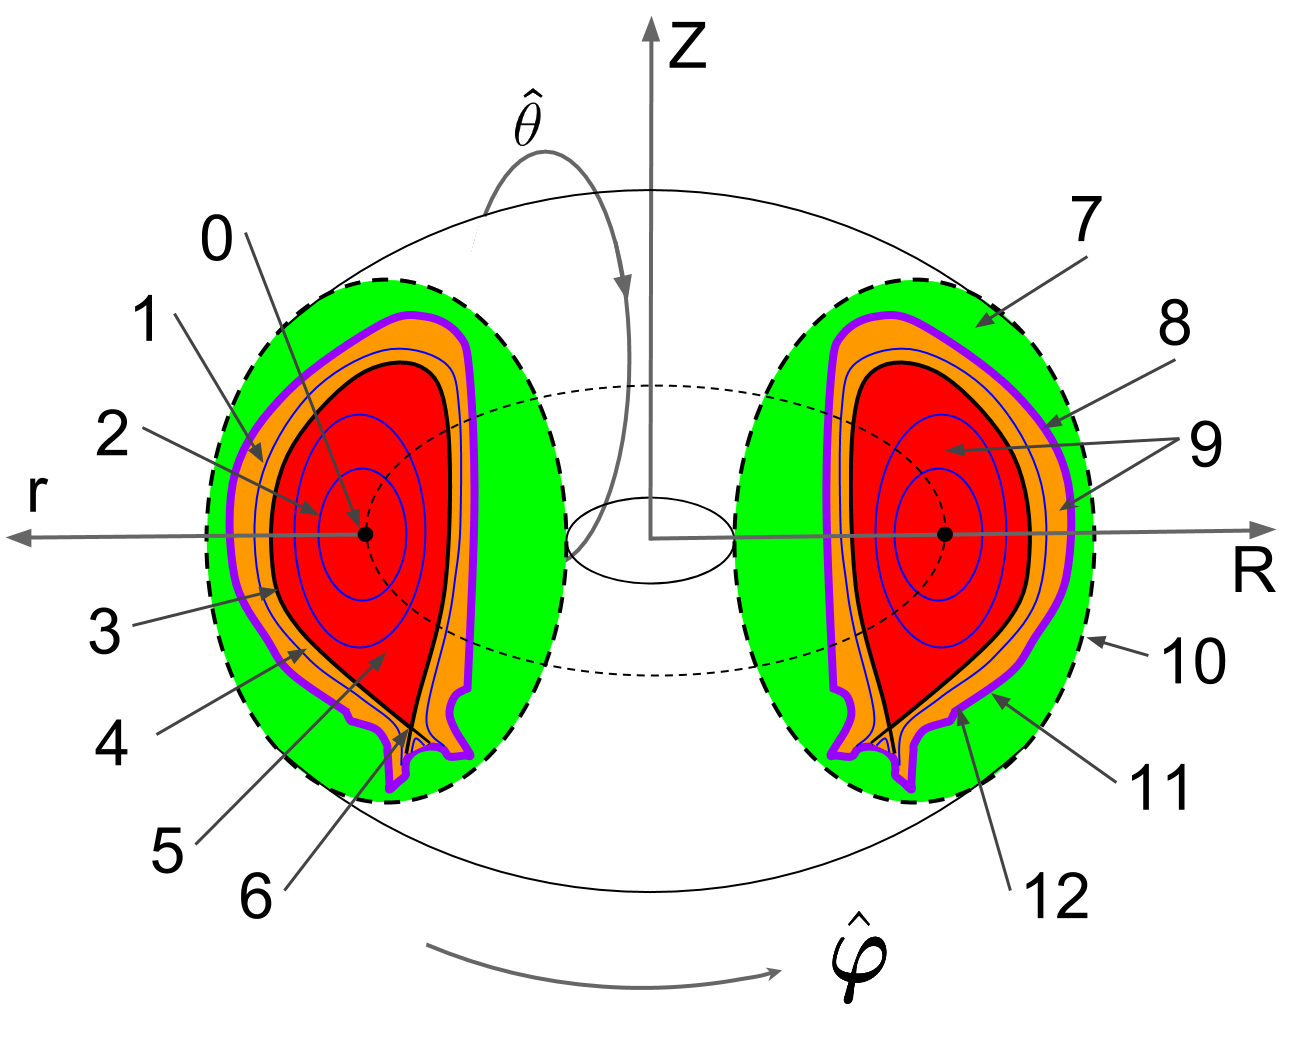
\includegraphics[width=3in]{fig/fusiongeo3d.png}
\caption{\small{Geometric components of the tokamak cross section (plane): (0) magnetic axis, (1) open flux surface, (2) closed flux surface,  (3) separatrix, (4) scrape-off layer, (5) plasma core, (6) $x$ point, (7) vacuum vessel, (8) wall region, (9) plasma region, (10) vacuum boundary, (11) outer wall boundary, (12) inner wall boundary}}
\label{fig:geo}
\end{figure}

The plasma region (9 in Figure \ref{fig:geo}) is bounded by the limiter or the boundary of the material wall (12 in Figure \ref{fig:geo}) \cite{wesson2011tokamaks}. There exists the closed flux surface or a separatrix in plasma (2 and 3 in Figure \ref{fig:geo}) and  it further splits the region into two distinct regions: the scraped-off layer and the plasma core (4 and 5 in Figure \ref{fig:geo}) \cite{wesson2011tokamaks}. The flux surfaces in the plasma core are concentric loops between the magnetic axis (0 in Figure \ref{fig:geo}) and the separatrix. The surfaces are distorted away by the $x$ point (6 in Figure \ref{fig:geo}) which is a saddle point of the magnetic flux on the separatrix.  There can be more than one $x$ points existing on the separatrix in general situations. The scrape-off layer is the region between the separatrix and the wall boundary. Flux surfaces end at the wall in this region and the outermost surface coincide with the wall. 7 and 8 in Figure \ref{fig:geo} depict a vacuum vessel and wall region.  

The geometry for M3D-$C^1$ is managed by the library, \emph{pumi\_geom}, which represents a geometric model as a hierarchy of topological entities of \emph{regions, shells, faces, loops, edges, vertices}, and \emph{use} entities for vertices, edges, loops and faces. 

\begin{figure}
\center
\begin{tabular}{ccc}
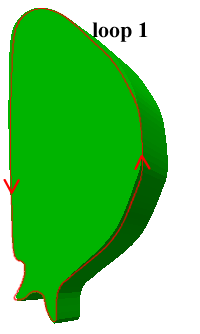
\includegraphics[scale=0.3]{fig/plasmaGeoRegion.png}&
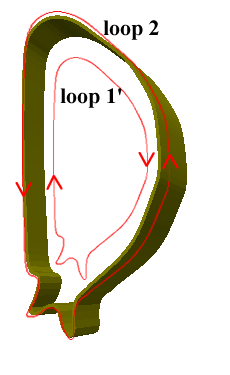
\includegraphics[scale=0.3]{fig/wallGeoRegion.png}&
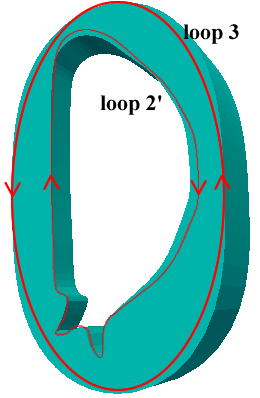
\includegraphics[scale=0.3]{fig/vacuumGeoRegion.png}\\
\small{(a) plasma face}&\small{(b) wall face}&\small{(c) vacuum vessel face}\\
\end{tabular}
\caption{\small{Geometric faces on a plane}} 
\label{fig:facetopo}
\end{figure}

\begin{figure}
\center
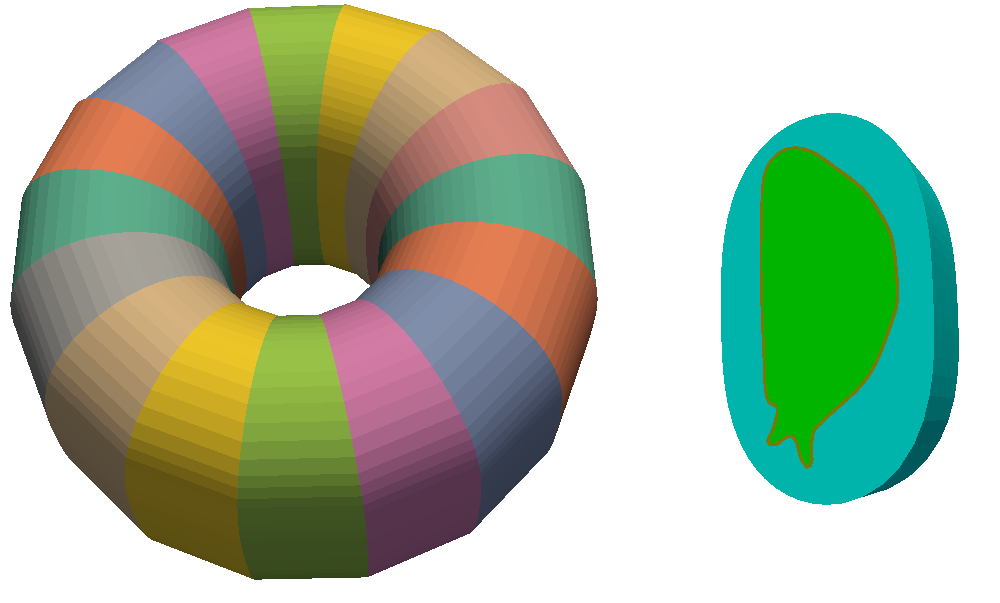
\includegraphics[width=3in]{fig/3dGeoTorus.png}
\caption{\small{3D torus with 16 planes and the regions between planes}}
\label{fig:3dtopo}
\end{figure}

\begin{itemize}
\item There are three faces on a plane. The inner plasma face is bounded by the loop on the inner material wall (Figure \ref{fig:facetopo}(a)). The wall face is bounded by two loops on the inner and outer material walls (Figure \ref{fig:facetopo}(b)). The outer vacuum face is bounded by the loop on the outer material wall and the loop on the vacuum vessel (Figure \ref{fig:facetopo}(c)). The loops that two faces contact on the plane are formed by the same group of edges in the opposite directions. 

\item In 3D, torus gemetry is composed by geometric regions between the planes that correspond to vacuum, wall and plasma region in the tokamak reactor. The left figure in Figure \ref{fig:3dtopo} illustrates an example 3D torus with 16 planes (left), and geometric regions between two planes corresponding to the plasma, wall and vacuum vessel (right).

\item Each geometric region is bounded by a shell that is made up of two faces on the neighboring planes and a number of faces between planes (Figure \ref{fig:regiontopo}). The faces between planes are on the boundaries of the material wall or the vacuum. Therefore, the torus geometry is \emph{non-manifold} \cite{weiler1986topo} in that there are faces bounding two regions. 
\item A geometric face between planes is either bounded by a loop that is made up of two edges on the planes and two edges between planes (Figure \ref{fig:facetopobtw}(a)), or two loops on the planes (Figure \ref{fig:facetopobtw}(b)).
\end{itemize}

In addition to the topological representation, the shape information is used to define the complete geometric model, which includes the positions of the model vertices, the geometry of the curves associated with the model edges, and the geometry of the surfaces associated with the model faces, etc. Ideally, in M3D-$C^1$, the geometry of the wall curves would be defined in the reactor's CAD model. Currently the wall curves is defined by an ordered set of points and the points are interpolated by the B-splines \cite{prautzsch2002bezier}. In the current implmenentation, the wall curves are defined by analytic functions where the curve of the vacuum boundary is defined as a simple smooth loop formed by B-spline given the user-specified width and height. The surfaces are either planar or formed by revolving the curves along the torus axis.
\begin{figure}
\center
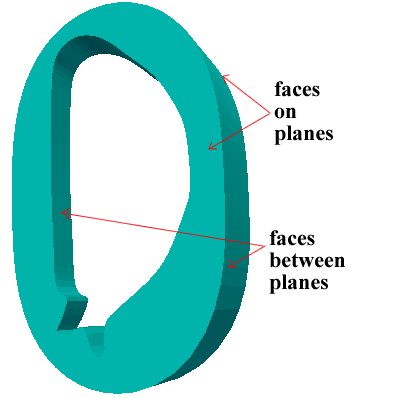
\includegraphics[width=2in]{fig/vacuumGeoRegionFace.png}
\caption{\small{Geometric region of vacuum vessel between two planes}}
\label{fig:regiontopo}
\end{figure}

\begin{figure}
\center
\begin{tabular}{cc}
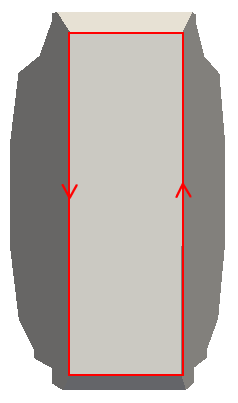
\includegraphics[width=1in]{fig/facebtw1.png}&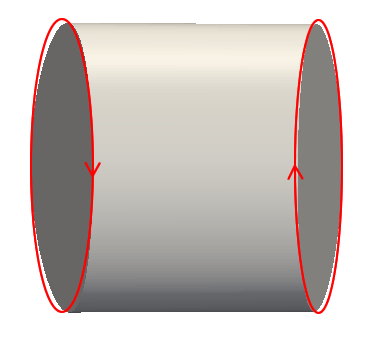
\includegraphics[width=1.7in]{fig/facebtw2.png}\\
\small{(a) bounded by a loop}&\small{(b) bounded by two loops}\\
\end{tabular}
\caption{\small{Geometric faces between planes}}
\label{fig:facetopobtw}
\end{figure}

%+++++++++++++++++++++++++++++++++++++++++++++++++++++
\subsection{Mesh}\label{sec:mesh}
%+++++++++++++++++++++++++++++++++++++++++++++++++++++

%+++++++++++++++++++++++++++++++++++++++++++++++++++++
\subsubsection{2D mesh generation}
%+++++++++++++++++++++++++++++++++++++++++++++++++++++
The initial 2D mesh for a cross section of tokamak is generated by the Simmetrix meshing tool \cite{simmetrix-web-page} then uniformly refined if needed. The initial mesh is further improved by applying the local modification iteratively until the mesh meets the desired size field \cite{li2003accounting,li20053d,alauzet2006parallel,sahni2007automated}. Currently, a mesh size field is defined from the toroidal magnetic flux field $\psi$. A normalized flux field is defined by $\tilde{\psi}=\frac{\psi-\psi_0}{\psi_l-\psi_0}$, where $\psi_l$ and $\psi_0$ is the field value at the plasma boundary and the magnetic axis. The mesh size normal to the surface $h_1$ and the mesh size tangent to the surface $h_2$ is defined as

\begin{equation}
h_i^{-1}=\tilde{h}_i^{-1}+\frac{1}{l_{ci}\left(1+\frac{\tilde{\psi}-\psi_c}{W_c}\right)^2}, \quad i=1,2
\end{equation}

where $l_{ci}$, $\psi_c$ and $W_c$ are constants. 
$\tilde{h}_i$ is defined by
\begin{eqnarray}
\tilde{h}_i&=&b_i[1-e^{|\frac{\tilde{\psi}}{a}-1|^2)}]+c_i, \quad \tilde{\psi}<a,\, \text{inside plasma} \nonumber \\ 
\tilde{h}_i&=&d_i[1-e^{|\frac{\tilde{\psi}}{a}-1|^2)}]+c_i, \quad \tilde{\psi}>a, \, \text{outside plasma}
\end{eqnarray}
where $b_i$, $d_i$, $a$ and $c_i$ are constants. The constant parameters of the equations are determined such the adapted mesh has finer size at the plasma boundary and the region that the instability may happen. Since there is richer physics in the normal direction of the flux surface than the other direction, the directional mesh size field are defined to represent this property.

\begin{figure}
\center
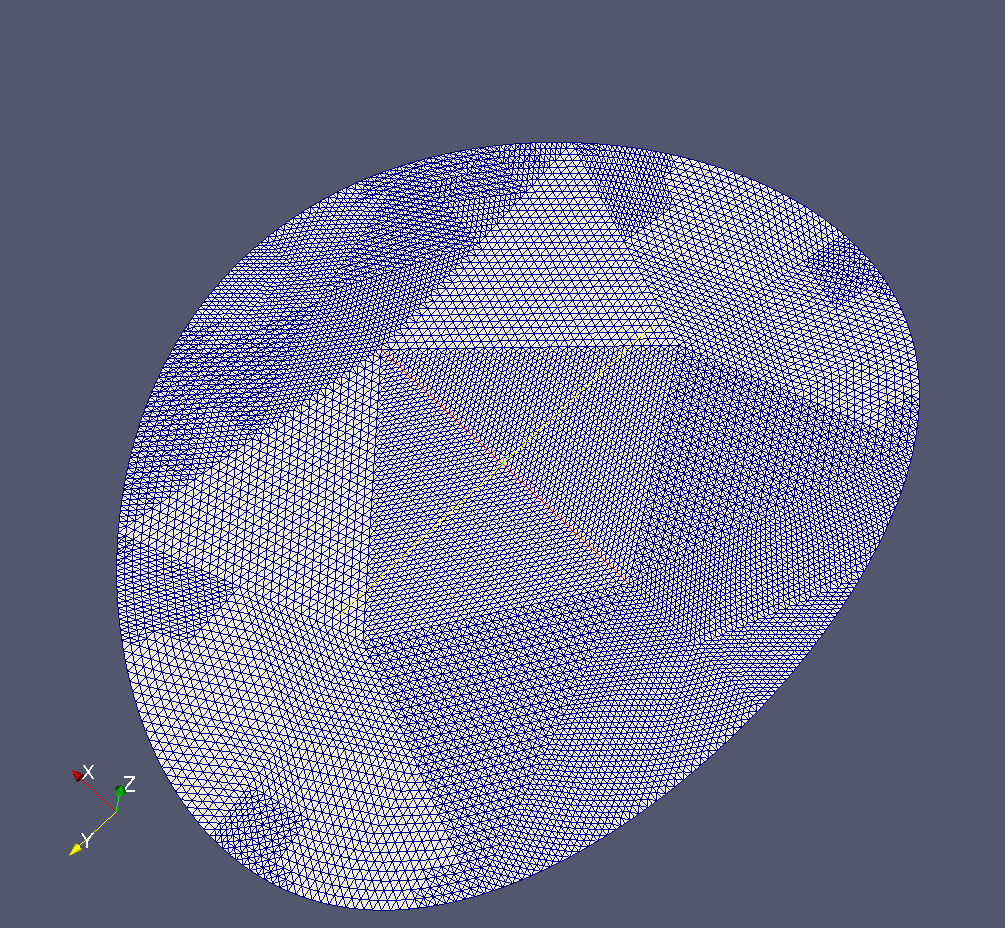
\includegraphics[width=3in]{fig/2d.png}
\caption{\small{Example of a 2D plane loaded on four processes}}
\label{fig:2d-plane}
\end{figure}

To run 2D simulation on $N$ processes, the 2D mesh is partitioned into $N$ parts so each process loads a part. Figure~\ref{fig:2d-plane} illustrates an example 2D mesh with 12,261 vertices, 36,406 edges and 24,146 triangles loaded on 4 processes.

%+++++++++++++++++++++++++++++++++++++++++++++++++++++
\subsubsection{3D mesh construction}
%+++++++++++++++++++++++++++++++++++++++++++++++++++++
For $N$-part distributed 2D mesh, each 2D mesh is loaded onto a \emph{process group} which consists of $N$ processes. The steps to construct 3D mesh out of $P$ 2D planes are the following:
\begin{enumerate}
\item 3D geometric model construction - $P$ cross sections are constructed by changing the toroidal angles. Geometric edges, faces and regions are created between the cross sections.
\item On each process group, the remote copy of mesh vertices, edges and faces on next process group are created and the owner copies are set to mesh vertices, edges and faces on next process group.
\item mesh edges, faces and regions between planes are created.
\item Part boundary links are set and the partition model is re-newed based on new 3D mesh partitioning topology.
\end{enumerate}

Using eight 2D planes in Figure~\ref{fig:2d-plane}, Figure \ref{fig:3d-plane} illustrates 3D mesh constructed on 32 processes. The resulting 3D mesh consists of 98,088 vertices, 391,512 edges, 486,568 faces, and 193,168 regions. 

\begin{figure}
\center
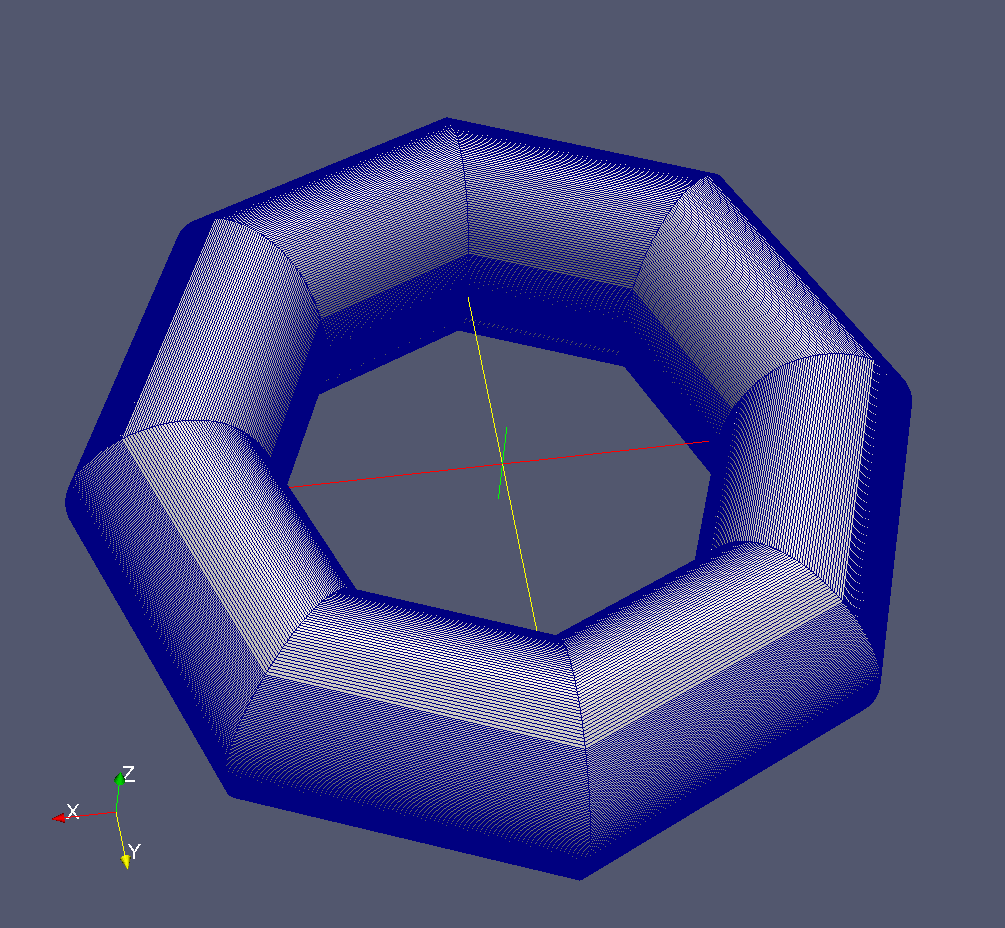
\includegraphics[width=3in]{fig/3d.png}
\caption{\small{Example 3D mesh constructed with 8 planes}}
\label{fig:3d-plane}
\end{figure}


%+++++++++++++++++++++++++++++++++++++++++++++++++++++
\section{PDE Discretization in M3D-$C^1$} \label{sec:m3dc1_dis}
%+++++++++++++++++++++++++++++++++++++++++++++++++++++
This section discusses the discretization of Equation \ref{eqn:mhd} (component C in Figure \ref{fig:femstructure})) in temporal and spatial dimensions.
%+++++++++++++++++++++++++++++++++++++++++++++++++++++
\subsection{Linearized Semi-implicit Time Stepping Method} \label{sec:timestep}
%+++++++++++++++++++++++++++++++++++++++++++++++++++++
The temporal discretization of the equation set \ref{eqn:mhd} is performed by the linearized $\theta$-advanced method \cite{ferraro2009calculations}. We take the velocity equation \ref{eqn:velocity} for example to illustrate the process.

Substitute the discretized variables with the form as
\begin{eqnarray}
  \frac{\partial \mathbf{V}} {  \partial t} &=&  \frac{\mathbf{V}^{n+1}-\mathbf{V}^{n}} { \delta t} \\
   \mathbf{V} &=&(1-\theta)\mathbf{V}^{n} + \theta \mathbf{V}^{n+1} = \mathbf{V}^n + \theta(\mathbf{V}^{n+1}-\mathbf{V}^n) \\
   \mathbf{J} &=&\mathbf{J}^m + \theta(\mathbf{J}^{m+1}-\mathbf{J}^m) \\
    \mathbf{B} &=&\mathbf{B}^m + \theta(\mathbf{B}^{m+1}-\mathbf{B}^m) \\
  p &=& p^m + \theta(p^{m+1}-p^m) \\
\end{eqnarray}
into Equation \ref{eqn:velocity}. 
Equation \ref{eqn:velocity} is discretized in the temporal dimension as (drop the $\mathbf{\Pi}$ term and assume constant $n$ here for simplicity)
\begin{eqnarray}
nM_i \left\{( \frac{\mathbf{V}^{n+1}-\mathbf{V}^{n} } { \delta t} ) 
+ \left[\mathbf{V}^n + \theta(\mathbf{V}^{n+1}-\mathbf{V}^n) \right] \cdot \nabla \left[\mathbf{V}^n + \theta(\mathbf{V}^{n+1}-\mathbf{V}^n)  \right] \right\}  \nonumber \\
+ \nabla \left[p^m + \theta(p^{m+1}-p^m) \right]  \nonumber \\
= \left[\mathbf{J}^m + \theta(\mathbf{J}^{m+1}-\mathbf{J}^m) \right] \times \left[ \mathbf{B}^m + \theta(\mathbf{B}^{m+1}-\mathbf{B}^m) \right]   \label{eqn:velocity2}
\end{eqnarray}

The equation is nonlinear with respect to unknown variables $()^{n+1}$ and $()^{m+1}$. For example, the terms of $\mathbf{V}^{n+1}\cdot \nabla \mathbf{V}^{n+1}$ are nonlinear.

Consider $()^{n+1}-()^n \sim \delta t$ and $()^{m+1}-()^m \sim \delta t$, the equation is linearized by dropping the term of order $\delta t^2$. The linearized temporal-discretized equation of \ref{eqn:velocity2} is

\begin{eqnarray}
nM_i \left\{ \mathbf{V}^{n+1}   +\theta \delta t  (\mathbf{V}^n \cdot \nabla \mathbf{V}^{n+1} + \mathbf{V}^{n+1} \cdot\nabla \mathbf{V}^{n})  \right\}    \nonumber \\
  \theta \delta t  \nabla p^{m+1} -  \theta \delta t (\mathbf{J}^{m+1}\times \mathbf{B}^m+\mathbf{J}^{n}\times \mathbf{B}^{m+1})  \nonumber \\
      = nM_i  \mathbf{V}^{n}  - (1-2 \theta) \delta t  \mathbf{V}^n \cdot \nabla \mathbf{V}^{n}
 -(1-\theta) \delta t  \nabla p^{m}  \nonumber \\
 +(1-2\theta) \delta t  \mathbf{J}^{m}\times \mathbf{B}^m. \label{eqn:velocityLin}
\end{eqnarray}

The equation is linearized with respect to the unknown  variables $()^{n+1}$ and $()^{m+1}$. Notice that $\mathbf{J}$ can be substituted by Equation \ref{eqn:jeqn}.

Perform the same procedure to the whole equation set \ref{eqn:mhd} and use $m=n$. We obtain ``unsplit $\theta$-implicit'' method in \cite{ferraro2009calculations}. It leads to a linear system of the equations with all the unknown variables $(n, \mathbf{V}, \mathbf{B}, p_e, p_i)$. 

The semi-implicit form is obtained by advancing the unknown variables separately.  The equation of the magnetic field (Equation \ref{eqn:mag}) and the equation of the pressure (Equation \ref{eqn:press_e} and \ref{eqn:press_i}) are used to eliminate the $\mathbf{B}^{m+1}$ and $\mathbf{p}^{m+1}$ in \ref{eqn:velocityLin}.

$\mathbf{E}$ is approximated by Equation \ref{eqn:elec} as $\mathbf{E}=-\mathbf{u}\times \mathbf{B}$ (drop the other terms for ideal MHD). Substitute the expression of $\mathbf{E}$ into Equation \ref{eqn:mag} and it is used to obtain $\mathbf{B}^{m+1}$ as
\begin{equation}
\frac{\mathbf{B}^{m+1}-\mathbf{B}^m}{\delta t} = \nabla \times \left\{\left[\mathbf{u}^{n}+ \theta (\mathbf{u}^{n+1}-\mathbf{u}^n)\right] \times \mathbf{B}^m \right\}.
\end{equation}
$\mathbf{B}^{m+1}$ is obtained as
\begin{equation}
\mathbf{B}^{m+1}=\mathbf{B}^m+ \delta t (1-\theta) \nabla \times \mathbf{u}^{n}  \times \mathbf{B}^m + \theta \delta t  \nabla \times \mathbf{u}^{n+1}  \times \mathbf{B}^m \label{eqn:bn1} 
\end{equation}

Substitute Equation \ref{eqn:bn1} into Equation \ref{eqn:velocityLin}, we get
\begin{eqnarray}
nM_i \left\{ \mathbf{V}^{n+1}   +\theta \delta t  (\mathbf{V}^n \cdot \nabla \mathbf{V}^{n+1} + \mathbf{V}^{n+1} \cdot\nabla \mathbf{V}^{n})  \right\}     \nonumber \\
  \theta \delta t  \nabla p^{m+1} -  \theta^2 \delta t^2 \mathcal{L}^{B}(\mathbf{V}^{n+1})   \nonumber \\
      = nM_i  \mathbf{V}^{n}  - (1-2 \theta) \delta t  \mathbf{V}^n \cdot \nabla \mathbf{V}^{n}
 -(1-\theta) \delta t  \nabla p^{m}   \nonumber \\
 -\alpha \delta t^2 \mathcal{L}^{B}(\mathbf{V}^{n})  + \delta t   \frac{1}{\mu_0}(\nabla \times \mathbf{B}^m)  \times \mathbf{B}^m, \label{eqn:velocityLinSplit}
\end{eqnarray}
where $ \mathcal{L}^{B} (\mathbf{V})= \frac{1}{\mu_0}[\nabla \times \nabla \times (\mathbf{V} \times \mathbf{B}^{m})]\times \mathbf{B}^n +  \frac{1}{\mu_0} (\nabla \times \mathbf{B}^m) \times [\nabla \times (\mathbf{V} \times \mathbf{B}^{m})] $ is the contribution of $\mathbf{B}$ to the linear ideal MHD operator  $\mathcal{L}$ in \cite{ferraro2009calculations},  and $\alpha =\theta(1-\theta)$.

Similarly, $p^{m+1}$ can be eliminated from Equation \ref{eqn:velocityLinSplit}. The unknown variable in the equation only involves $\mathbf{V}^{n+1}$ and we have

\begin{eqnarray}
nM_i \left\{ \mathbf{V}^{n+1}   +\theta \delta t  (\mathbf{V}^n \cdot \nabla \mathbf{V}^{n+1} + \mathbf{V}^{n+1} \cdot\nabla \mathbf{V}^{n})  \right\}     \nonumber \\
   -  \theta^2 \delta t^2 (\mathcal{L}^B+\mathcal{L}^{p})(\mathbf{V}^{n+1})   \nonumber \\
      = nM_i  \mathbf{V}^{n}  - (1-2 \theta) \delta t  \mathbf{V}^n \cdot \nabla \mathbf{V}^{n}
    \nonumber \\
 -\alpha \delta t^2 (\mathcal{L}^{B}+\mathcal{L}^{p})(\mathbf{V}^{n})  + \delta t  \left[ \frac{1}{\mu_0}(\nabla \times \mathbf{B}^m)  \times \mathbf{B}^m  - \nabla p ^m \right], \label{eqn:velocityLinSplit2}
\end{eqnarray}
where $\mathcal{L}^{p} = \nabla (\mathbf{V} \cdot \nabla p + \Gamma p \nabla \cdot \mathbf{V})$ is  the contribution of $p$ to the linear ideal MHD operator  $\mathcal{L}$  in \cite{ferraro2009calculations}.

Define linear differential operators as
\begin{subequations} 
\begin{eqnarray}
\mathcal{S}_v (\mathbf{V})&=& nM_i \left\{ \mathbf{V}  +\theta \delta t  (\mathbf{V}^n \cdot \nabla \mathbf{V} + \mathbf{V}\cdot\nabla \mathbf{V}^{n})  \right\}  
   -  \theta^2 \delta t^2 \mathcal{L}(\mathbf{V})  \\
\mathcal{D}_v (\mathbf{V})&=&  nM_i  \left\{ \mathbf{V}  - \frac{(1-2 \theta)}{2} \delta t ( \mathbf{V}^n \cdot \nabla \mathbf{V} +  \mathbf{V} \cdot \nabla \mathbf{V}^n ) \right\}  
 -\alpha \delta t^2 \mathcal{L}(\mathbf{V})  \\
 \mathcal{Q}_v (\mathbf{B}, p)&=& \delta t\frac{1}{\mu_0} \left\{\frac{1}{2} \left[(\nabla \times \mathbf{B})  \times \mathbf{B}^m + (\nabla \times \mathbf{B})^m  \times \mathbf{B}\right] - \nabla p \right\}.
\end{eqnarray}
\end{subequations}

Equation \ref{eqn:velocityLinSplit2} can be written as
\begin{equation}
\mathcal{S}_v (\mathbf{V}^{n+1}) = \mathcal{D}_v (\mathbf{V}^{n}) + \mathcal{Q}_v (\mathbf{B}^{m}, p^m).
\end{equation}

The above equation can be further transformed by splitting the variables into summation of the static solution at time 0 and the variation from the static solution \cite{ferraro2009calculations} as
\begin{subequations} 
\begin{eqnarray}
\mathbf{V} &=& \mathbf{V}^0+ \tilde{V} \\
n &=& n^0+ \tilde{n} \\
\mathbf{B} &=& \mathbf{B}^0+ \tilde{B} \\
p &=& p^0+ \tilde{p}.
\end{eqnarray}
\end{subequations}

The set of equations with more general terms discretized in the temporal dimension is summarized as follows. The velocity is advanced first. The density,  the total pressure, the magnetic field and the electric pressure are advanced from the updated velocity.
\begin{subequations}  \label{eqn:mhdTimeStepMatrixForm}
\begin{eqnarray}
\mathcal{S}_v (\mathbf{V}^{n+1})&=& \mathcal{D}_v (\mathbf{V}^{n}) + \mathcal{Q}_v (\mathbf{B}^{m}, p^m, n^m) + \mathbf{f}_v \\
\mathcal{S}_n (n^{m+1})&=& \mathcal{D}_n (n^{m}) + \mathcal{R}_n(\mathcal{V}^{n+1}) + \mathcal{Q}_n(\mathcal{V}^{n}) + f_n \\
\mathcal{S}_p (p^{m+1})&=& \mathcal{D}_p (p^{m}) + \mathcal{R}_p(\mathcal{V}^{n+1}) + \mathcal{Q}_p(\mathcal{V}^{n}) + f_p \\
\mathcal{S}_b (\mathbf{B}^{m+1}, p_e^{m+1})&=& \mathcal{D}_b (\mathbf{B}^{m}, p_e^m) + \mathcal{R}_b(\mathcal{V}^{n+1}) + \mathcal{Q}_b (\mathcal{V}^{n}) + \mathbf{f}_b,
\end{eqnarray}
\end{subequations}
where $\mathcal{S}$ is the left-hand-side linear differential operator, $\mathcal{D}$ is the right-hand-side linear differential operator on the same variable of each equation, $\mathcal{R}$ is the right-hand-side linear differential operator on the advanced velocity, and $\mathcal{Q}$ is the right-hand-side linear differential operator on other variables.

%+++++++++++++++++++++++++++++++++++++++++++++++++++++
\subsection{Spacial Discretization by $C^1$ Finite Elements} \label{sec:element}
%+++++++++++++++++++++++++++++++++++++++++++++++++++++

The $C^1$ finite elements are applied for spacial discretization in M3D-$C^1$. The $C^1$ reduced quintic triangle element \cite{jardin2004triangular} is used on the poloidal cross section of  the tokamak. The 3D $C^1$ wedge element is obtained by  introducing  the cubic Hermite polynomials in the toroidal direction to the $C^1$ reduced quintic triangle element  \cite{jardin2012multiple}. Figure \ref{fig:wedgeCurved} illustrates the wedge mesh element by connecting the triangle elements on two tokamak cross sections on the $RZ\varphi$ coordinate system. The $C^1$ finite elements associated with the mesh elements are discussed in the rest of the section. A comma is used to denote taking derivatives with respect to the subscript components for simplicity, e.g. ,$U_{,\eta} \equiv \frac{\partial U } {\partial \eta}$ and $U_{,\eta\eta} \equiv \frac{\partial^2 U}{ \partial \eta^2}$.

\begin{figure} 
\centering
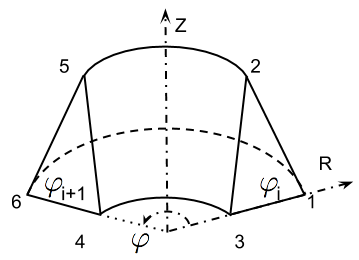
\includegraphics[width=2in]{fig/wedgeCurved.png}
\caption{\small{The wedge mesh element between two cross sections in M3D-$C^1$}}
\label{fig:wedgeCurved}
\end{figure} 

%+++++++++++++++++++++++++++++++++++++++++++++++++++++
\subsubsection{$C^1$ Reduced Quintic Triangle Element}
%+++++++++++++++++++++++++++++++++++++++++++++++++++++
\begin{figure} 
\centering
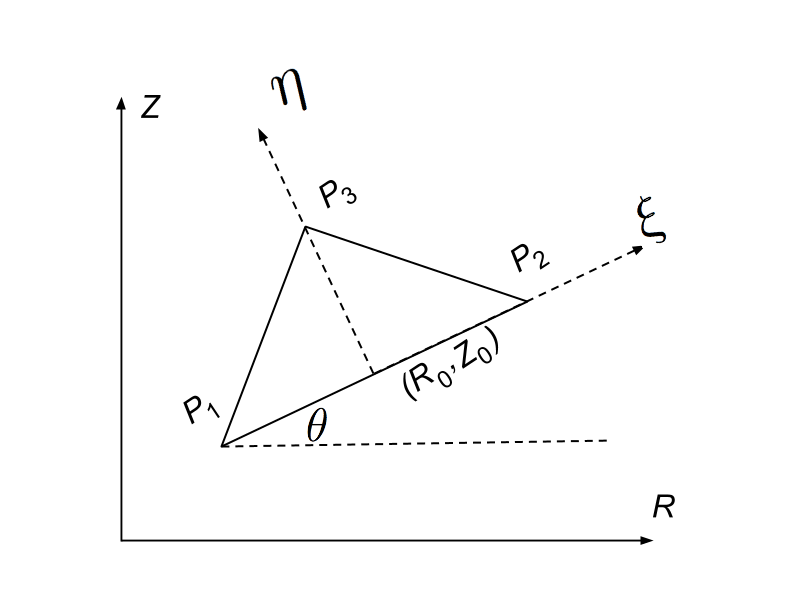
\includegraphics[width=3in]{fig/coordinate.png}
\caption{\small{The triangle element. $a$, $b$, $c$, and $\theta$ are four geometric parameters of the triangle.  $(\xi,\eta)$ is the local  coordinate, and $(R,Z)$~\cite{jardin2004triangular}.}}
\label{fig:coordinate}
\end{figure} 

A set of shape functions on the triangle with $5^{th}$-order polynomials is defined to have $C^1$ inter-element continuity. 
The mapping from the local coordinate $(\xi, \eta)$ to the global coordinate $(R,Z)$ is defined as
\begin{equation} \label{mapping}
\left[ \begin{array}{c}
          R\\
          Z
        \end{array}
 \right]=\left[
        \begin{array}{cc}
          cos(\theta) & -sin(\theta) \\
          sin(\theta) & cos(\theta)
        \end{array}
        \right] \left[
        \begin{array}{c}
          \xi \\
          \eta
        \end{array}  \right] +\left[\begin{array}{c}
          R_0\\
          Z_0
        \end{array}
        \right]
\end{equation}
where $(R_0,Z_0)$ is the origin point of the $(\xi, \eta)$ coordinate system in Figure \ref{fig:coordinate}.

Eighteen shape functions $\{ \mu_i \}$ that are $5^{th}$-order polynomials of $(\xi,\eta)$  need to be defined. The shape functions are expanded as
\begin{equation} \label{basisfunction}
\mu_i=\sum_{k=1}^{21}\alpha_{ki}\xi^{m_k}\eta^{n_k}, \quad 0\leq m_k+n_k\leq5, \quad i=1,2,...,18
\end{equation}

There are twenty-one coefficients $\{\alpha_{ki}\}$ in each $5^{th}$-order polynomial to be decided.  The coefficients are constrained to satisfy the following conditions.
\begin{itemize}
\item The function value ($\mu_i$), the two first-order derivatives (${\mu_i,_\xi}$ and $\mu_i,_{\eta}$) and the three second-order derivatives ($\mu_i,_{\xi\xi}$, $\mu_i,_{\xi\eta}$ and $\mu_i,_{\eta\eta}$) are evaluated at three vertices $(P_1,P_2,P_3)$. The eighteen values are prescribed such that only one value is one and all the others are zero.
\begin{equation}
\delta_{ij}=\sum_{k=1}^{21}\alpha_{ki} \mathcal{D}_{j}\{\xi^{m_k}\eta^{n_k}\}, \quad j=1,2...18
\end{equation}
where $\mathcal{D}_{j}$ is the differential operator which gets the value, the first derivative or the second derivative of the expression at the vertex of the triangle. 
\item The other three constraints require the normal derivatives of the shape functions reduce to a cubic polynomial such that  the normal derivatives along the edge can be solely determined by the DOF's attached to the two connected vertices. It guarantees the property of $C^1$ inter-element continuity.  Notice that one of the three constraints is equivalent to drop the term of $\xi^4\eta$ for all the shape functions.
\end{itemize}

\begin{figure}
\center
\begin{tabular}{cc}
\subfloat[function value]{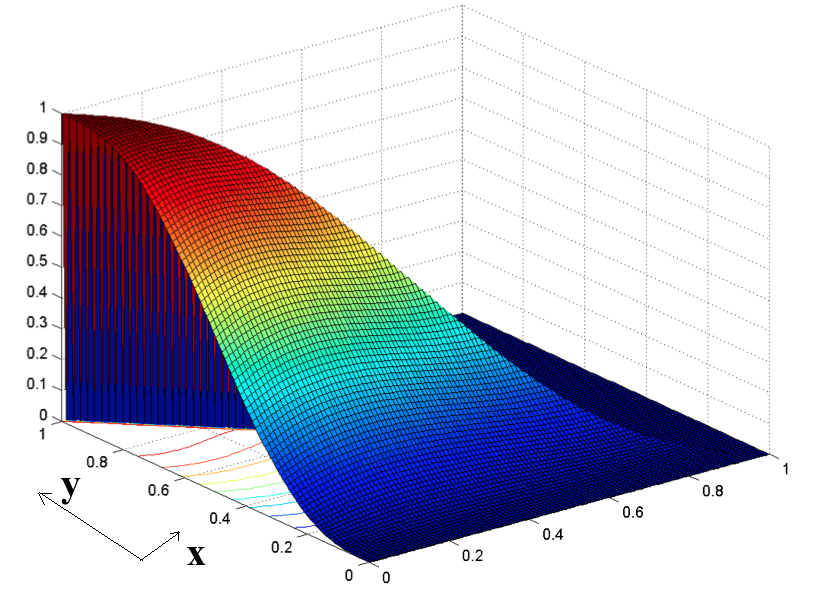
\includegraphics[height=0.25\textheight]{fig/shape1.png}}
 & \subfloat[$1^{st}$-order derivative in $x$ direction]{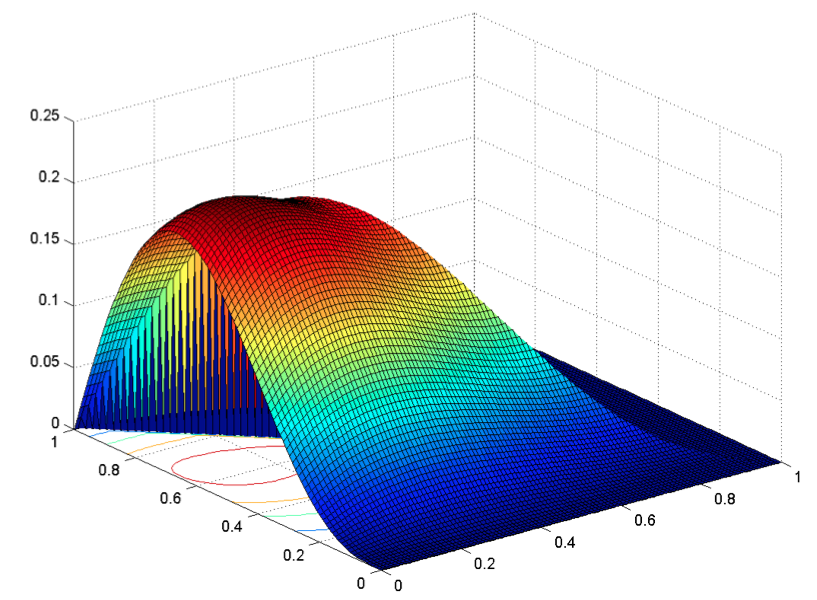
\includegraphics[height=0.25\textheight]{fig/shape2.png}} \\
 \subfloat[$1^{st}$-order derivative in $y$ direction]{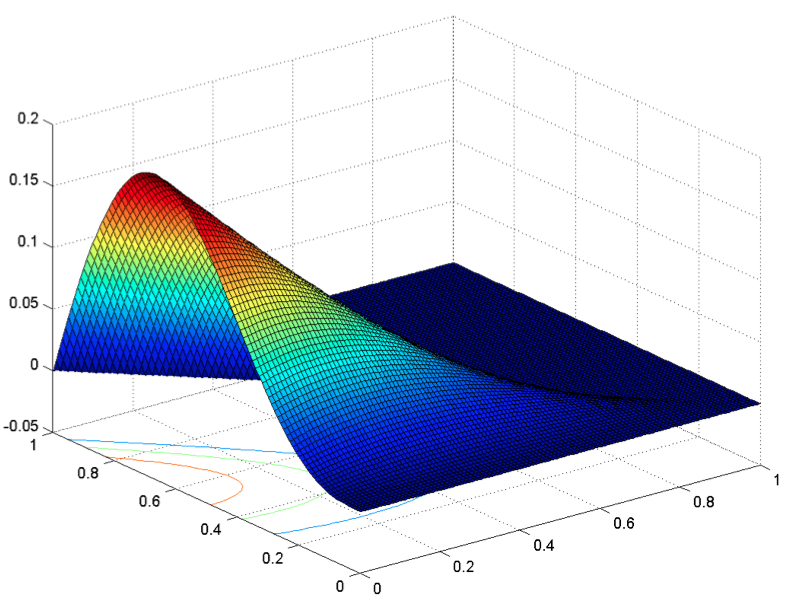
\includegraphics[height=0.25\textheight]{fig/shape3.png}}
 & \subfloat[$2^{nd}$-order derivative in $x$ direction]{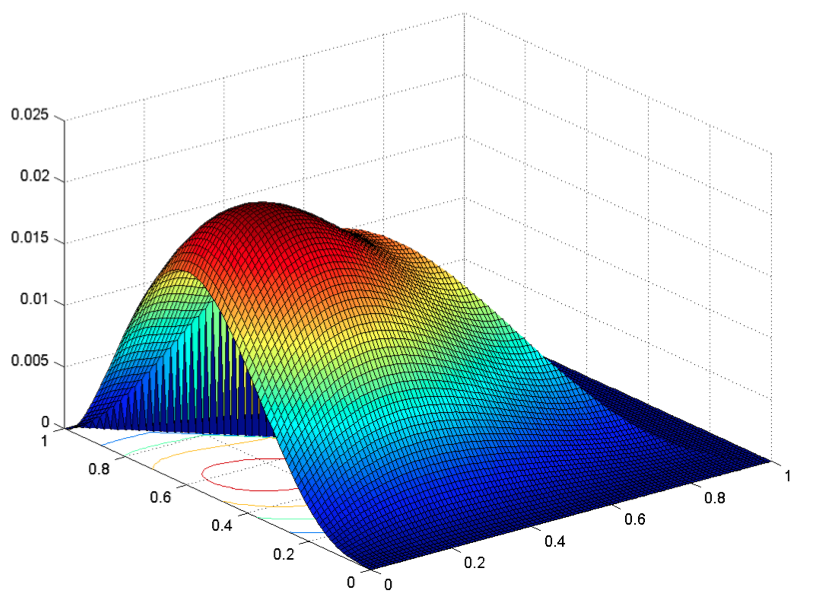
\includegraphics[height=0.25\textheight]{fig/shape4.png}} \\
  \subfloat[twisted derivative in $x$, $y$ direction]{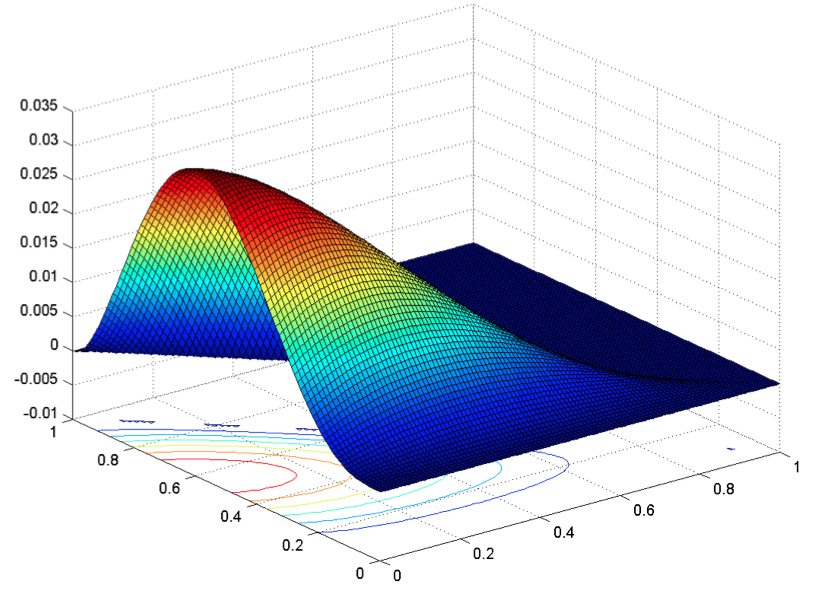
\includegraphics[height=0.25\textheight]{fig/shape5.png}}
 & \subfloat[$2^{nd}$-order derivative in $y$ direction]{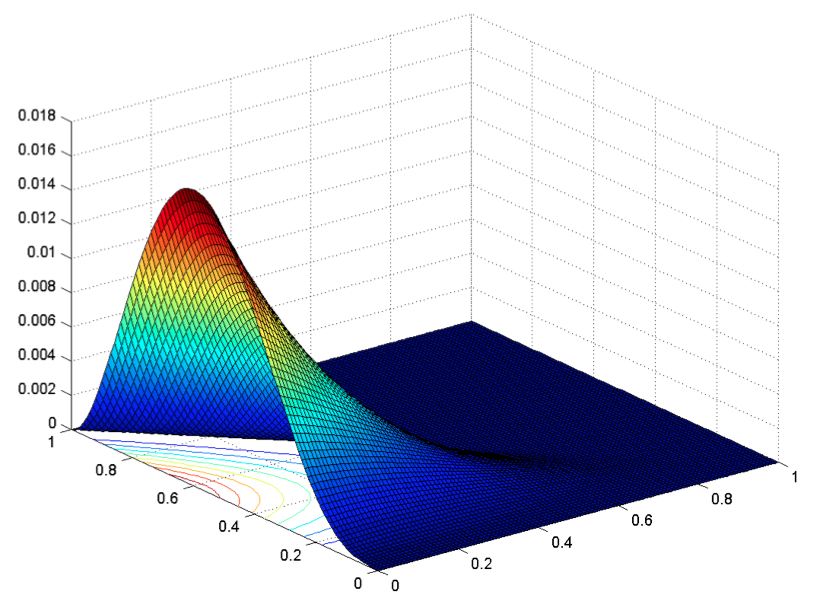
\includegraphics[height=0.25\textheight]{fig/shape6.png}} \\
\end{tabular}
\caption{\small{Shape functions on associated with vertex (0,1). All the sub-figures use the same axis.}}
\label{fig:figshape}
\end{figure}

Figure \ref{fig:figshape} plots the first six shape functions. It requires to solve a linear system with twenty unknowns (the coefficient of the term $\xi^4\eta$ is zero) to obtain the  coefficient of the fifth-order polynomials  for each shape function. The matrix of the linear system can be found in Appendix A of Reference \cite{jardin2004triangular}.  The order of polynomial completeness is fourth. 

A scalar field $U$ can be interpolated with the eighteen shape functions on the triangle as
\begin{equation} \label{field}
U(\xi,\eta)=\sum_{i=1}^{18}\lambda_i \mu_i(\xi,\eta),
\end{equation} 
where $\lambda_i$ is the multiplier associated with $\mu_i$. From the construction of the shape functions, $\{\lambda_i\}$ equals to the value of $U$, $U_{,\xi}$, $U_{,\eta}$, $U_{,\xi\xi}$, $U_{,\xi\eta}$, and $U_{,\eta\eta}$ at the three vertices respectively. The first six multipliers associated with vertex $P_1$ in Figure \ref{fig:coordinate} and the corresponding field values evaluated at the vertex are listed below.

\begin{center}
 \begin{tabular}{ |l|l|l|l|l|l|l|}
\hline
 multiplier & $\lambda_1$ & $\lambda_2$ & $\lambda_3$ & $\lambda_4$ & $\lambda_5$ &$\lambda_6$  \\ \hline
 field value & $U$ & $U_{,\xi}$ & $U_{,\eta}$ & $U_{,\xi\xi}$ & $U_{,\xi\eta}$ &$U_{,\eta\eta}$  \\ \hline
\end{tabular}
\end{center}

Eighteen DOFs are defined in the element. The DOFs equal to values of  $U,U_{,R}, U_{,Z}, U_{,RR}, U_{,RZ}, U_{,ZZ}$ at the three vertices respectively. The first six DOFs associated with vertex $P_1$ and the corresponding field values evaluated at $P_1$  are listed below.

\begin{center}
 \begin{tabular}{ |l|l|l|l|l|l|l|}
\hline
 DOF& $d_1$ & $d_2$ & $d_3$ & $d_4$ & $d_5$ &$d_6$  \\ \hline
 field value & $U$ & $U_{,R}$ & $U_{,Z}$ & $U_{,RR}$ & $U_{,RZ}$ &$U_{,ZZ}$  \\ \hline
\end{tabular}
\end{center}
It is not hard to find the relation between the multipliers of the shape functions and DOFs by utilizing the chain rule. For example,  from
\begin{eqnarray}
U_{,\xi}&=&U_{,R}R_{,\xi}+U_{,Z}Z_{,\xi}=U_{,R}cos(\theta)+U_{,Z}sin(\theta) \\
U_{,\xi\xi}&=&U_{,RR}R_{,\xi}^2+ U_{RZ}2R_{,\xi}Z_{,\xi}+U_{,ZZ}Z_{,\xi}^2 \\ \nonumber
               &=&U_{,RR}cos^2(\theta)+U_{,RZ}2sin(\theta)cos(\theta)+U_{,ZZ}sin^2(\theta),
\end{eqnarray}
we have
\begin{eqnarray}
\lambda_2 &=& cos(\theta)d_2+sin(\theta)d_3 \\
\lambda_4&=&cos^2(\theta)d_4+2sin(\theta)cos(\theta)d_5+sin^2(\theta)d_6.
\end{eqnarray}

The relation of the first six multipliers and the DOFs can be written in the matrix form as
\begin{equation} 
\left[
 \begin{array}{c}
 \lambda_{1} \\
 \lambda_{2} \\
 \lambda_{3} \\
 \lambda_{4}\\
 \lambda_{5}\\
 \lambda_{6}
 \end{array} \right]=\left[
 \begin{array}{cccccc}
 1 & 0 & 0 & 0 & 0 & 0 \\
 0 & cos(\theta) & sin(\theta) & 0 & 0 &0 \\
 0 & -sin(\theta) & cos(\theta) & 0 & 0 &0 \\
 0 & 0 & 0 & cos^2(\theta) & 2sin(\theta)cos(\theta) & sin^2(\theta) \\
 0 & 0 & 0 & -sin(\theta)cos(\theta) & cos^2(\theta)-sin^2(\theta) & sin(\theta)cos(\theta) \\
 0 & 0 & 0 & sin^2(\theta) & -2sin(\theta)cos(\theta) & cos^2(\theta) \\ 
 \end{array}
 \right]  \left[
 \begin{array}{c}
 d_{1} \\
 d_{2} \\
 d_{3} \\
 d_{4}\\
 d_{5}\\
 d_{6}
 \end{array} \right].
\end{equation}

\subsubsection{$C^1$ Cubic Hermite Polynomials in $\varphi$ Direction}

\begin{figure}
\center
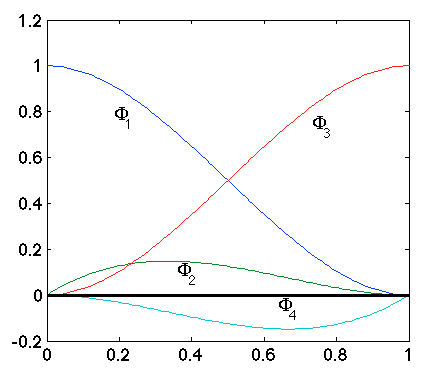
\includegraphics[width=2.5in]{fig/hermitecubic.png}
\caption{\small{Hermite cubic polynomials defined on $[0,1]$}} 
\label{fig:hermitecubic}
\end{figure}

The $C^1$ cubic Hermite polynomials are used to interpolate the field in the toroidal $\varphi$ direction (See Figure \ref{fig:geo} for the coordinate system).  Define $\tilde{\varphi}\in[0,1]$ as the local coordinate and the mapping to the global coordinate $\varphi$ as
\begin{equation}
\varphi = \varphi_{i} + (\varphi_{i+1}-\varphi_{i})\tilde{\varphi},
\end{equation}
where $\tilde{\varphi}_{i}$ and $\tilde{\varphi}_{i+1}$ are the toroidal angles of the two cross sections (Figure \ref{fig:wedgeCurved}).

Figure \ref{fig:hermitecubic} plots the shape functions defined on the interval $[0,1]$. The two shape functions associated with the point $\tilde{\varphi}=0$ are
\begin{eqnarray}
\Phi_1(\tilde{\varphi})&=&(\tilde{\varphi}-1)^2(2\tilde{\varphi}+1) \\
\Phi_2(\tilde{\varphi})&=&\tilde{\varphi}(\tilde{\varphi}-1)^2
\end{eqnarray}
such that $\Phi_1(0)=1,\Phi_1'(0)=\Phi_1(1)=\Phi_1'(1)=0$ 
and  $\Phi_2'(0)=1,\Phi_2(0)=\Phi_1(1)=\Phi_1'(1)=0$. The two shape functions associated with the point $\tilde{\varphi}=1$ are 
\begin{eqnarray}
\Phi_3(\tilde{\varphi})&=&\tilde{\varphi}^2(3-2\tilde{\varphi}) \\
\Phi_4(\tilde{\varphi})&=&\tilde{\varphi}^2(\tilde{\varphi}-1).
\end{eqnarray}

A scalar field $U$ can be interpolated with the four shape functions on the interval as
\begin{equation} \label{field}
U(\tilde{\varphi})=\sum_{i=1}^{4}\lambda_i \Phi_i(\tilde{\varphi}),
\end{equation} 
where $\lambda_i$ is the multiplier associated with $\Phi_i$. From the construction of the shape functions, $\{\lambda_i\}$  equal to the value of $U,U_{,\tilde{\varphi}}$ at the two points of the interval. The four multipliers associated with the two points $\tilde{\varphi}=0,1$ and the corresponding field values  are listed below.
\begin{center}
 \begin{tabular}{ |l|l|l|l|l|}
\hline
 multiplier & $\lambda_1$ & $\lambda_2$ & $\lambda_3$ & $\lambda_4$  \\ \hline
field value & $U(0)$ & $U,_{\tilde{\varphi}}(0)$ & $U(1)$ & $U,_{\tilde{\varphi}}(1)$ \\ \hline 
\end{tabular}
\end{center}

Four DOFs  are defined with the 1D cubic Hermite element with values equal to   $U,U_{,\varphi}$ at the two points respectively.   The DOFs and the corresponding field values on $[\varphi_i, \varphi_{i+1}]$ are listed below (here $U'\equiv U,_{\varphi}$ is used).
\begin{center}
 \begin{tabular}{ |l|l|l|l|l|}
\hline
 DOFs & $d_1$ & $d_2$ & $d_3$ & $d_4$   \\ \hline
field value & $U(\varphi_i)$ & $U'(\varphi_i)$ & $U(\varphi_{i+1})$ & $U'(\varphi_{i+1})$ \\ \hline 
\end{tabular}
\end{center}
It is not hard to find the relation between $\lambda_i$ and $d_i$ for the cubic Hermite element from the chain rule as
\begin{eqnarray}
\lambda_1 &=& d_1 \\
\lambda_2 &=& (\varphi_{i+1}-\varphi_{i}) d_2 \\
\lambda_3 &=&  d_3 \\
\lambda_4 &=& (\varphi_{i+1}-\varphi_{i}) d_4. 
\end{eqnarray}
\subsubsection{3D $C^1$ Element} 
The 3D $C^1$ element is defined on the wedge (Figure \ref{fig:wedgeCurved}) by combining the $C^1$ triangle element and the $C^1$ Hermite polynomials. 
Define the local coordinate $(\xi,\eta,\tilde{\varphi})$  and the mapping to the global coordinate $(R,Z,\varphi)$ as
\begin{equation} \label{mapping}
\left[ \begin{array}{c}
          R\\
          Z \\
          \varphi
        \end{array}
 \right]=\left[
        \begin{array}{ccc}
          cos(\theta) & -sin(\theta) & \\
          sin(\theta) & cos(\theta) & \\
          & &  \varphi_{i+1}-\varphi_{i}
        \end{array}
        \right] \left[
        \begin{array}{c}
          \xi \\
          \eta \\
          \tilde{\varphi}
        \end{array}  \right] +\left[\begin{array}{c}
          R_0\\
          Z_0\\
          \varphi_i
        \end{array}
        \right]
\end{equation}

Interpolate  the field U in the wedge mesh element (Figure \ref{fig:wedgeCurved}) with the shape functions of the $C^1$ triangle $\{\mu_i\}$ and the cubic Hermite $\{\Phi_i\}$  as
\begin{equation}
U(\xi,\eta,\tilde{\varphi})=\left(\sum_{i=1}^{18} \alpha_i \mu_i(\xi,\eta) \right) \cdot \left( \sum_{j=1}^{4} \beta_j \Phi_j (\tilde{\varphi}) \right),
\end{equation}
where $\alpha_i$ and $\beta_j$ are coefficients of  $\mu_i$ and $\Phi_j$ respectively.

It can be further written as
\begin{equation}
U=\sum_{i=1}^{18} \sum_{j=1}^{4} \lambda_{ij} \mu_i(\xi,\eta)\Phi_j(\tilde{\varphi}),
\end{equation}
where $\lambda_{ij}=\alpha_i\beta_j$ is the multiplier of the shape function $\mu_i(\xi,\eta)\Phi_j(\tilde{\varphi})$.

There are totally seventy-four ($18\times4$) multipliers in the wedge elements. From the properties of $\mu_i$ and $\Phi_j$, the seventy-four multipliers  equal to the values of $U$,  $U_{,\xi}$,  $U_{,\eta}$, $U_{,\xi\xi}$,  $U_{,\xi\eta}$, $U_{,\eta\eta}$,  $U_{,\tilde{\varphi}}$, $U_{,\xi\tilde{\varphi}}$, $U_{,\eta\tilde{\varphi}}$, $U_{,\xi\xi\tilde{\varphi}}$, $U_{,\xi\eta\tilde{\varphi}}$ and $U_{,\eta\eta\tilde{\varphi}}$ evaluated at the six vertices of the wedge mesh element. The twelve multipliers associated with vertex $1$ in Figure \ref{fig:wedgeCurved} and the corresponding field values evaluated at the vertex are listed below.
\begin{center}
 \begin{tabular}{ |l|l|l|l|l|l|l|}
\hline
 multiplier & $\lambda_{11}$ & $\lambda_{21}$ & $\lambda_{31}$ & $\lambda_{41}$ & $\lambda_{51}$ &$\lambda_{61}$  \\ \hline
 field value & $U$ & $U_{,\xi}$ & $U_{,\eta}$ & $U_{,\xi\xi}$ & $U_{,\xi\eta}$ &$U_{,\eta\eta}$  \\ \hline
 multiplier & $\lambda_{12}$ & $\lambda_{22}$ & $\lambda_{32}$ & $\lambda_{42}$ & $\lambda_{52}$ &$\lambda_{62}$  \\ \hline
 field value & $U,_{}\tilde{\varphi}$ & $U_{,\xi\tilde{\varphi}}$ & $U_{,\eta\tilde{\varphi}}$ & $U_{,\xi\xi\tilde{\varphi}}$ & $U_{,\xi\eta\tilde{\varphi}}$ &$U_{,\eta\eta\tilde{\varphi}}$  \\ \hline
\end{tabular}
\end{center}
 
Seventy-four DOFs are defined in the $C^1$ wedge element. The DOFs equal to values of  $U$, $U_{,R}$, $U_{,Z}$, $U_{,RR}$, $U_{,RZ}$, $U_{,ZZ}$, $U,_{\varphi}$, $U_{,R\varphi}$, $U_{,Z\varphi}$, $U_{,RR\varphi}$, $U_{,RZ\varphi}$ and $U_{,ZZ\varphi}$ at the six vertices respectively. The first twelve DOFs associated with vertex $1$  in Figure \ref{fig:wedgeCurved}  and the corresponding field values evaluated at the vertex  are listed below.
\begin{center}
 \begin{tabular}{ |l|l|l|l|l|l|l|}
\hline
 DOF& $d_1$ & $d_2$ & $d_3$ & $d_4$ & $d_5$ &$d_6$  \\ \hline
 field value & $U$ & $U_{,R}$ & $U_{,Z}$ & $U_{,RR}$ & $U_{,RZ}$ &$U_{,ZZ}$  \\ \hline
  DOF& $d_7$ & $d_8$ & $d_9$ & $d_{10}$ & $d_{11}$ &$d_{12}$  \\ \hline
 field value & $U,_{\varphi}$ & $U_{,R\varphi}$ & $U_{,Z\varphi}$ & $U_{,RR\varphi}$ & $U_{,RZ\varphi}$ &$U_{,ZZ\varphi}$  \\ \hline
\end{tabular}
\end{center}

It is not hard to find the relation between the multipliers of the shape functions and DOFs by utilizing the chain rule. The relation of first twelve DOFs and multipliers is given by

\begin{equation} 
\left[
 \begin{array}{c}
 \lambda_{11} \\
 \lambda_{21} \\
 \lambda_{31} \\
 \lambda_{41}\\
 \lambda_{51}\\
 \lambda_{61}
 \end{array} \right]
=\left[
 \begin{array}{cccccc}
 1 & 0 & 0 & 0 & 0 & 0 \\
 0 & cos(\theta) & sin(\theta) & 0 & 0 &0 \\
 0 & -sin(\theta) & cos(\theta) & 0 & 0 &0 \\
 0 & 0 & 0 & cos^2(\theta) & 2sin(\theta)cos(\theta) & sin^2(\theta) \\
 0 & 0 & 0 & -sin(\theta)cos(\theta) & cos^2(\theta)-sin^2(\theta) & sin(\theta)cos(\theta) \\
 0 & 0 & 0 & sin^2(\theta) & -2sin(\theta)cos(\theta) & cos^2(\theta) \\ 
 \end{array}
 \right]
 \left[
 \begin{array}{c}
 d_{1} \\
 d_{2} \\
 d_{3} \\
 d_{4}\\
 d_{5}\\
 d_{6}
 \end{array} \right],
\end{equation}
and
\begin{equation} 
\left[
 \begin{array}{c}
 \lambda_{12} \\
 \lambda_{22} \\
 \lambda_{32} \\
 \lambda_{42}\\
 \lambda_{52}\\
 \lambda_{62}
 \end{array} \right]
=c\left[
 \begin{array}{cccccc}
 1 & 0 & 0 & 0 & 0 & 0 \\
 0 & cos(\theta) & sin(\theta) & 0 & 0 &0 \\
 0 & -sin(\theta) & cos(\theta) & 0 & 0 &0 \\
 0 & 0 & 0 & cos^2(\theta) & 2sin(\theta)cos(\theta) & sin^2(\theta) \\
 0 & 0 & 0 & -sin(\theta)cos(\theta) & cos^2(\theta)-sin^2(\theta) & sin(\theta)cos(\theta) \\
 0 & 0 & 0 & sin^2(\theta) & -2sin(\theta)cos(\theta) & cos^2(\theta) \\ 
 \end{array}
 \right]
 \left[
 \begin{array}{c}
 d_{7} \\
 d_{8} \\
 d_{9} \\
 d_{10}\\
 d_{11}\\
 d_{12}
 \end{array} \right],
\end{equation}
where $c=\varphi_{i+1}-\varphi_{i}$.

%+++++++++++++++++++++++++++++++++++++++++++++++++++++
\section{Forming/Solving Global Discrete Equations} \label{sec:form-eq}
%+++++++++++++++++++++++++++++++++++++++++++++++++++++


%\textcolor{red}{Fan: why do we have this paragraph on the DOF  mapping?} Although PETSc provides a variety of tools that help to manage the mapping among the various numbering systems, M3D-$C^1$ relies on the ordering features on SCOREC libraries instead of PETSc. The approaches are:
%\begin{itemize}
%\item[-] PUMI and APF keep the global vertex ordering and DOF ordering consistent. For instance, for a vertex of global ID $i$ with $d$ DOF data, the global DOF ID's are $i$$\times$$d$, ..., $(i+1)$$\times$$d$$-$$1$, where $0$$\le$$i$$\le$$N-1$ and $N$ is the number of global vertices.
%\item[-] Two schemes available for vertex ordering - natual ordering (vertex order from mesh generator) or adjacency-based ordering on local process.
%\end{itemize}


\textit{\textcolor{blue}{Mark: This section needs to be sure to very carefully discuss
exactly what information about the dof's and their coupling is required
to most effectively construct the PETSc "matrix" which will be in some
form of sparse storage (banded, skyline, full sparse, ???). Until we
fully understand this we have no idea what we are doing or why. Thus
this must be the focus of what is being looked at and carefully
documented. Note, that are likely to be multiple options, we need to
carefully understand and use the one that makes the most sense.
In looking at previously developed code, I would tend to look carefully
at stuff done in the past since I know that if Nate implemented it, it
is likely done with one of the best approached.
Get me that technical information on that PETSc stuff as soon as possible.}}

The element contributions to the stiffness matrix and the force vector are assembled to form the global discrete equation. A global DOF ordering that assigns integer labels to DOFs associated with the mesh vertex is calculated. The integer corresponds to the equation number in the global discrete system.  The global discrete system is solved to get the solution fields (for instance, velocity and magnetic field) at the current time step.

%\begin{figure}
%\center
%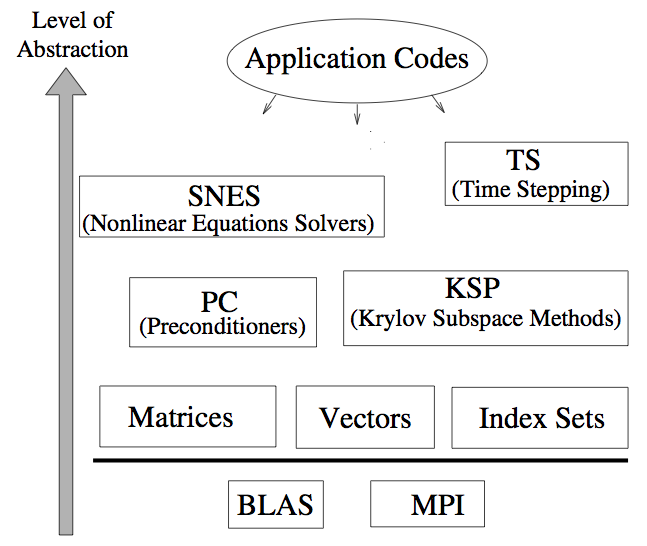
\includegraphics[width=3.5in]{fig/petsc-sw.png}
%\caption{\small{Organization of the PETSc libraries -- cites \textcolor{red}{Fan: not sure it's proper to use the PETSc figure here.}}}
%\label{fig:petsc-sw}
%\end{figure}

PETSc is  widely used as the solver program for partial differential equations and sparse matrix computation. 
% I do n't think it is proper to put it here --Fan
%As depicted in Figure~\ref{fig:petsc-components}, PETSc consists of a variety of numerical libraries where each library consists of numerical components that manipulate a particular set of data and operations. The key features include \cite{petsc-ug}:
%\begin{itemize}
%\item[-] Index sets for indexing into vectors, renumbering, etc.
%\item[-] Parallel vectors and matrices
%\item[-] Scatters/Gathers for communicating ghost point information
%\item[-] Sparse storage formats
%\item[-] Scalable parallel preconditioners including multi-grid and sparse direct solvers
%\item[-] KSP (Krylov subspace method)
%\item[-] Parallel non-linear solvers
%\item[-] Parallel time-stepping solvers
%\end{itemize}

%\begin{figure}
%\center
%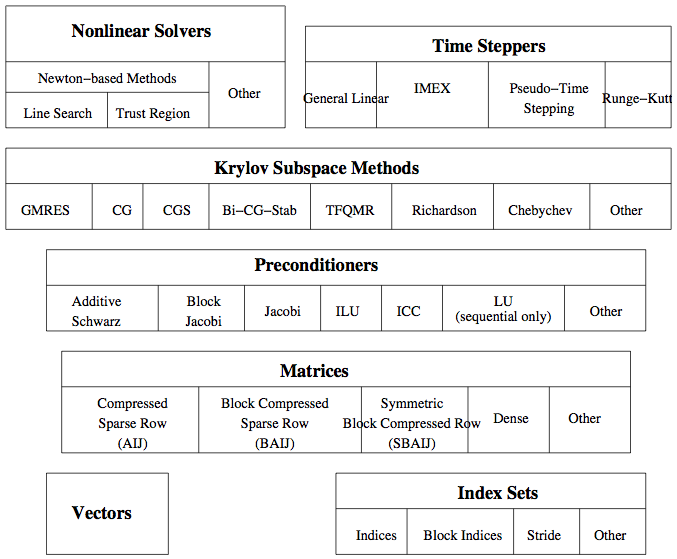
\includegraphics[width=5in]{fig/petsc-components.png}
%\caption{\small{Numerical components of PETSc (figure adopted from ~\cite{petsc-ug})}}
%\label{fig:petsc-components}
%\end{figure}

M3D-$C^1$ uses PETSc for the following purposes. 
\textit{(\textcolor{blue}{Fan: we have our own implementations of the matrix storage, parallel assembly procedure, and matrix-vector multiplication (item 2 and 3). But it may make more sense to let PETSc handle all these aspects.})} \textit{(\textcolor{blue}{Mark: I expect that is true. They have been doing it for years.})}
\begin{enumerate}
\item vector set up (\emph{Vec} objects)  in the linear system of the equations described in Equation \ref{eqn:sys}. See Section 7.1. %PETSc vectors (\emph{Vec} objects) are used to store the field variables.
\item matrix implementation (under development): PETSc matrices (\emph{Mat} objects) are used to store Jacobians and other sparse matrices. Matrix operations such as parallel assembly are performed through PETSc. See Section 7.2.
\item matrix-vector multiplication (under development): $D\mathbf{u}^n$ in Equation \ref{eqn:sys}  is calculated through PETSc function \emph{MatMult}.
\item solver of linear systems of equations: $S \mathbf{u}^{n+1} = \mathbf{b}$  in Equation \ref{eqn:sys}, where $\mathbf{b} = D \mathbf{u}^n +\mathbf{f}$, is solved with KSP component of PETSc. KSP provides combination of direct method, a Krylov subspace iterative method and a preconditioner. See Section 7.3.
\end{enumerate}

%\subsection{Indexing and Ordering}
%In parallel PDE codes, there is extra complexity caused by having multiple ways of indexing (numbering) and ordering objects such as vertices and degrees of freedom. For example, as depicted in Figure~\ref{fig:petsc-ordering}, a grid generator or partitioner may renumber the nodes, requiring adjustment of the other data structures that refer to these objects. In addition, local numbering (on a single process) of objects may be different than the global (cross-process) numbering. PETSc provides a variety of tools that help to manage the mapping among the various numbering systems. The two most basic are the \emph{AO (application ordering)}, which enables mapping between different global (cross-process) numbering schemes and the \emph{ISLocalToGlobalMapping}, which allows mapping between local (on-process) and global (cross-process) numbering~\cite{petsc-ug}.
%
%\begin{figure}
%\center
%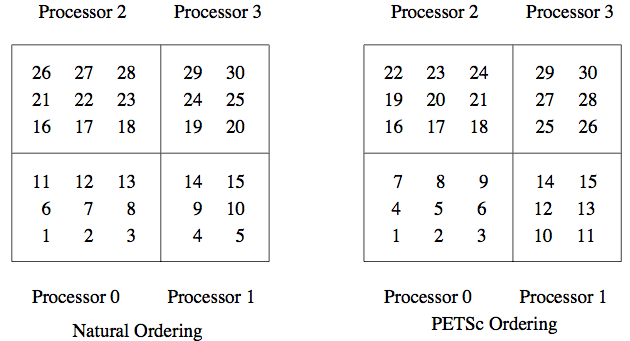
\includegraphics[width=4in]{fig/petsc-ordering.png}
%\caption{\small{Natural ordering and PETSc ordering for a 2D distributed array (four processes)~\cite{petsc-ug}}}
%\label{fig:petsc-ordering}
%\end{figure}

\subsection{Parallel Vectors}
Parallel vectors in PETSc are intended for discrete solution fields, the right-hand side of the linear systems, etc \cite{petsc-ug}. While APF is used as the general field management in parallel adaptive analysis, the usage lies in setting up the  parallel PETSc vectors through API functions (see Section \ref{sec:step4}) that  interact with APF such that the vectors can be used for solving a linear system or performing matrix-vector multiplication.

The values of vectors are obtained by \emph{m3dc1\_ent\_getdofdata} defined in Section \ref{sec:step4}. The indices of vectors are given by \emph{m3dc1\_field\_getglobaldofid} that returns the same global DOF ordering to construct the matrix in Equation \ref{eqn:sys}.

\subsection{Parallel Matrix}
Both the left-hand-side matrix ($S$ in Equation \ref{eqn:sys}) and the right-hand-side matrix ($D$ in Equation \ref{eqn:sys}) are formed explicitly in M3D-$C^1$.

\subsubsection{Hierarchical Block Structure of Matrix } \label{sec:blockstructure}
The matrices in M3D-$C^1$ exhibit a block structure in a hierarchical way.  If we can  take advantage of  the structure in multiple levels,  improvements may be made with regarding to the matrix storage (see Section \ref{sec:petscMatStore})  and the solving process (see Section \ref{sec:2dproblem}). 

There are three levels in the hierarchical block structure of the matrix.

Firstly, the $C^1$ finite elements assign multiple DOFs to mesh nodes to represent a scalar variable.  Each mesh node associates with six DOFs on the 2D mesh and twelve DOFs on the 3D mesh (see Section \ref{sec:element}). The block size at this level is six or twelve.

 Secondly, a physics quantity is decomposed into multiple scalar variables. For example, the velocity is  decomposed into three scalar variables $(U,\omega, \chi)$ (Equation \ref{eqn:scalarDecompsition}). The block size at this level is eighteen on the 2D mesh and thirty-six on the 3D mesh for the velocity. 
 
 Last, the construction of the 3D mesh by connecting meshes on planes dictates the matrix is in a way of cyclic tri-diagonal blocks (Figure \ref{fig:3DMatrix}).  The block size at this level is  thirty-six  multiplied by the number of the mesh nodes on a cross section for the velocity. Notice that the block at this level is not dense. Each block is a sparse matrix formed by the sub-blocks at the second level. 

\begin{figure}[hbt]
\center
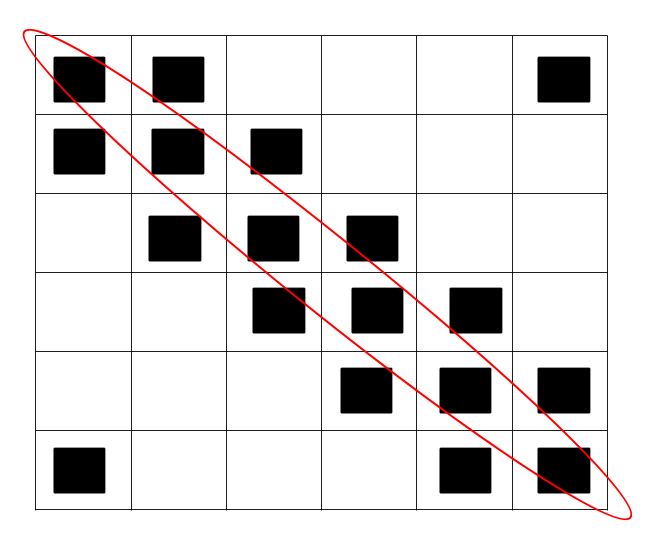
\includegraphics[width=0.4\textwidth]{fig/3DMatrix.png}
\caption{3D Matrix structure with six cross sections in the torus geometry. Each diagonal block corresponds to a 2D cross section.} \label{fig:3DMatrix}
\end{figure} 

%+++++++++++++++++++++++++++++++++++++++++++++++++++++
\subsubsection{Parallel Matrix Layout in PETSc} \label{sec:petsMatLayout}
%+++++++++++++++++++++++++++++++++++++++++++++++++++++

Each process ``owns'' a range of continuous rows in the PETSc matrix \cite{petsc-web-page}.  The matrix layout is illustrated in Fig. \ref{fig:petscMatLayout}.
The matrix layout  is decided based on the mesh partition and the global DOF ordering on the partitioned mesh. The mesh is partitioned to balance the process load and minimize the communication between part boundary \cite{zhou2012unstructured}. The global  DOF ordering on the partitioned mesh gives the row and column indices in the matrix.  Each process ``owns'' a continuous range of DOFs. It first calculates the starting DOF index, and orders the DOFs ``owned'' by the process. The DOFs indices are synchronized on the  part boundary.  Figure \ref{fig:2d-mesh-psim} illustrates the global DOF ordering on a partitioned mesh. Assume DOF 1 is ``owned'' by process 1 and DOF 3 is ``owned'' by process 2.  Process 1 will own rows 1 and 2 and process 2 will own row 3 and 4 in the matrix.

\begin{figure}
\center
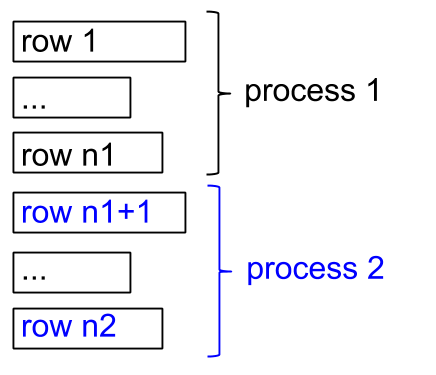
\includegraphics[width=1.7in]{fig/petscMatLayout.png}
\caption{\small{PETSc matrix layout}} 
\label{fig:petscMatLayout}
\end{figure}
\begin{figure}
\center
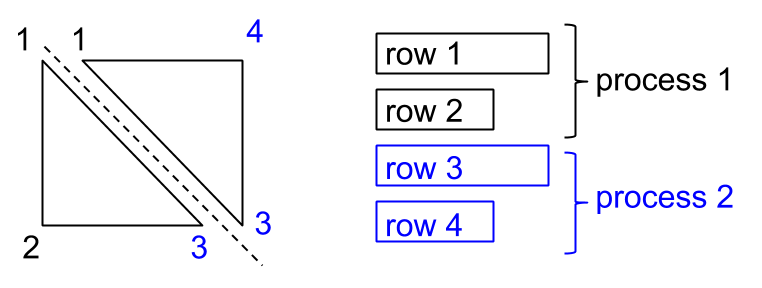
\includegraphics[width=3in]{fig/partitionedMeshSim.png}
\caption{\small{Global DOF ordering and matrix layout on a mesh partitioned and loaded by 2 processes. Assume DOFs attached to mesh nodes and one DOF per mesh node.}} 
\label{fig:2d-mesh-psim}
\end{figure}

%+++++++++++++++++++++++++++++++++++++++++++++++++++++
\subsubsection{Matrix Format Options} \label{sec:petscMatStore}
%+++++++++++++++++++++++++++++++++++++++++++++++++++++
%General matrix storage formats are discussed in this section.  The formats supported by PETSc are focused. 
The matrix can be represented in the following format.
\begin{itemize}
\item dense matrix (supported by PETSc):  the storage is analogous to a 2D array without considering the sparsity of the matrix. It is not used here.
\item band matrix (not supported by PETSc): the diagonal band of the matrix is stored. 
\item skyline matrix (not supported by PETSc):  the bandwidth of each column is maintained and all the matrix entries fall in the bandwidth are stored. It \cite{watkins2004fundamentals} is popularly used to store the symmetric positive definite matrices from the finite element codes in the area of structural mechanics. It preserves the same structure as the original matrix  in  the Cholesky decomposition.  An ordering of DOF that cluster the $non$-$zero$ values to the diagonal as close as possible is desired to reduce the memory to store the matrix.   Reordering algorithms such as the reverse Cuthill-McKee algorithm \cite{cuthill1969reducing} are applied to reduce the storage size. 
\textit{\textcolor{blue}{(Fan: General sparse methods instead of skyline are desired for very large system. See \url{http://en.wikipedia.org/wiki/Skyline_matrix}})}
\item general sparse matrix (supported by PETSc): only the $non$-$zero$ values and their positions in the matrix are stored. The sparse matrix storage in PETSc is discussed in the rest of the section.
\end{itemize}

The basic format of the sparse matrix in PETSc \cite{petsc-web-page} is the  compressed sparse row storage (CSR, or Yale Sparse Matrix format).  Three arrays $(\mathbf{A}, \mathbf{IA}, \mathbf{JA})$ are maintained to store the number of $non$-$zero$ values in each row, the starting index of each row and the column indices of the each $non$-$zero$ value respectively.  See \url{http://en.wikipedia.org/wiki/Sparse_matrix}  for detailed descriptions. 

When multiple  variables with different meanings are coupled, the sparse matrix can be  represented in a block way.  The block matrix is generally more efficient for problems with multiple DOFs per node. Considering there are multiples DOFs  associated with each mesh node,  block CSR is a more efficient way to store the matrix in M3D-$C^1$.  With block CSR, only the index of each block needs to be stored. For example, if there are 18 DOFs per node, the block size  is $18\times18$. It needs $324$ units of space in the array of column indices for a single block with size $18\times18$ if the matrix is not stored in a block way. However, it only needs one unit of space to store the column index if the matrix is stored in a block way.  

The array storing the $non$-$zero$ values ($\mathbf{A}$) and the array storing column indices ($\mathbf{JA}$) are two largest arrays in the CSR format.  Given the block size as $N_b$, the block CSR format can reduce the size of $\mathbf{JA}$ by a factor of $N_b^2$.  Considering $\mathbf{JA}$ uses single-precision integers, and $\mathbf{A}$ uses double-precision floating-points, the block storage of the original matrix can save the memory up to $25\%$ compared to the format without blocks.  

\begin{figure}
\center
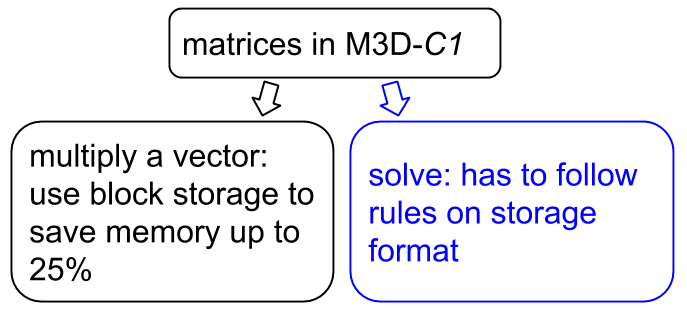
\includegraphics[width=3in]{fig/matTypes.png}
\caption{\small{Two purpose of matrices in M3D-$C^1$}} 
\label{fig:matTypes.png}
\end{figure}

The real improvement of the matrix storage may not be as high as $25\%$. There are two purposes of matrices created by M3D-$C^1$ (Figure \ref{fig:matTypes.png}). If the matrices are to multiply a vector, the matrices can use block CSR storage. If the matrices are to solve a linear system of equations, there are limitations of the specific storage formats. For example,  solving procedures that use SuperLU  do not support block CSR format. \footnote{need to confirm with PETSc developer with regards to the latest version.} The Table in \url{http://www.mcs.anl.gov/petsc/documentation/linearsolvertable.html} lists requirements of  specific algorithms on the matrix storage types. Notice that the table can be extended based on user request. 

The  \emph{preallocation} step tells PETSc the number of $non$-$zero$ values in the diagonal and off-diagonal portions of the sub-matrices (Figure \ref{fig:sparseMatrix}).  Accurate  preallocation reduces the number of dynamic memory allocation and copying data between memory blocks \cite{petsc-web-page}. Therefore, \emph{preallocation} is a crucial step to use  PETSc sparse matrices efficiently (no matter the sparse matrix is in block or not).


\begin{figure}
\center
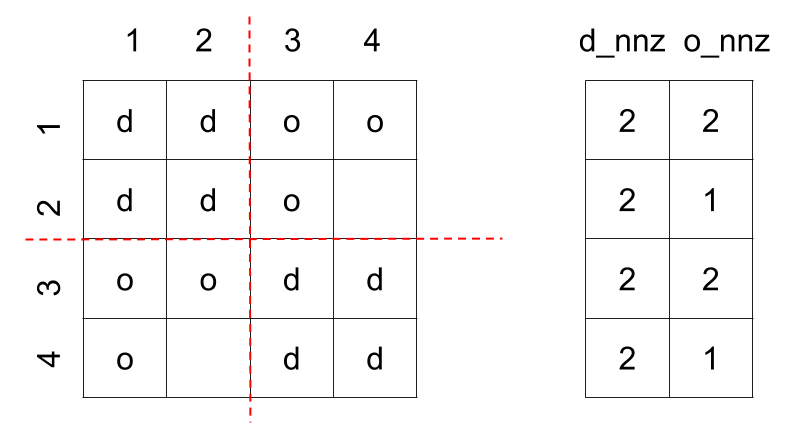
\includegraphics[width=3in]{fig/sparseMatrix.png}
\caption{\small{Preallocation of the sparse matrix from the mesh in Figure \ref{fig:2d-mesh-psim}.  Process 1 owns rows 1 and 2 and process 2 owns row 3 and 4 in the matrix. $d\_nnz$ is number of $non$-$zero$ values in the diagonal portion of local sub-matrix; $o\_nnz$ is number of $non$-$zero$ values in the off-diagonal portion of local sub-matrix.}} 
\label{fig:sparseMatrix}
\end{figure}

 The sparse matrix in the finite element analysis is obtained by assembling the contributions of the individual element. If the row and the column of the matrix correspond to two mesh nodes in the same element, there is a $non$-$zero$ value in the matrix at the location specified by the row and the column.  The algorithm to calculate the $non$-$zero$ values based on mesh adjacency is illustrated below. Here, we use the second-order adjacency (see Reference~\cite{Seol2014}), that is,  node A is  adjacent to node B, if A and B  are in the closure of the same mesh element.  

\begin{samepage}
\begin{verbatim}
procedure CACULATE_NNZ_MESH (DOFNODE, DNNZ, ONNZ)
    var DOFNODE = {number of DOFs per node}
    array DNNZ = {number of non-zero values in the diagonal portion}
    array ONNZ = {number of non-zero values in the off-diagonal portion}
    for P = 1 to number of nodes in the mesh part
        DNNZ(P) = the number of adjacent mesh nodes
                  belong to the same element owned by the process 
    end for
    collect DNNZ for the same mesh node over all the processes
    get the  number of adjacent mesh nodes in the whole mesh for each node
    put the result in ONNZ
    for P=1 to number of nodes in the mesh part
        ONNZ(P) = ONNZ(P) - DNNZ(P)
        DNNZ(P) =  DNNZ(P) + 1 (including the node self)
    end for
    for P=1 to number of nodes in the mesh part
        ONNZ(P) = ONNZ(P) * DOFNODE
        DNNZ(P) =  DNNZ(P) * DOFNODE
    end for
end procedure
\end{verbatim}
\end{samepage}

 We give two examples as follows. Assumes one DOF per mesh node.
 
For the 2D mesh in Figure \ref{fig:2d-mesh-psim}, node $1$ has two adjacent mesh nodes on the mesh part and three  adjacent mesh nodes on the whole mesh. One of the  two adjacent mesh nodes on the mesh part is owned by the process.   We have $o_{nnz}  = 3 - 1=2$ and $d_{nnz}=1+1=2$ for node 1 (see Figure \ref{fig:sparseMatrix}).

For 3D mesh with wedge element, each triangle on the 2D plane is connected to two triangles on the neighboring planes to form wedge elements (Figure \ref{fig:3DElment}).  Assume the 3D mesh is generated from $n$ 2D meshes in  Figure \ref{fig:2d-mesh-psim}. Node $1$ on plane $1$ connects to nodes on plane $2$ and plane $n$. Node 1 has $11$ adjacent nodes in the 3D mesh.  The number of  adjacent mesh nodes owned by the process  on the mesh part  is $1$  (same as the 2D mesh).  We have $d_{nnz}=1+1=2$, and $o_{nnz}  = 11 - 1 =10$ (see Figure \ref{fig:sparseMatrix3D}). 

\begin{figure}
\center
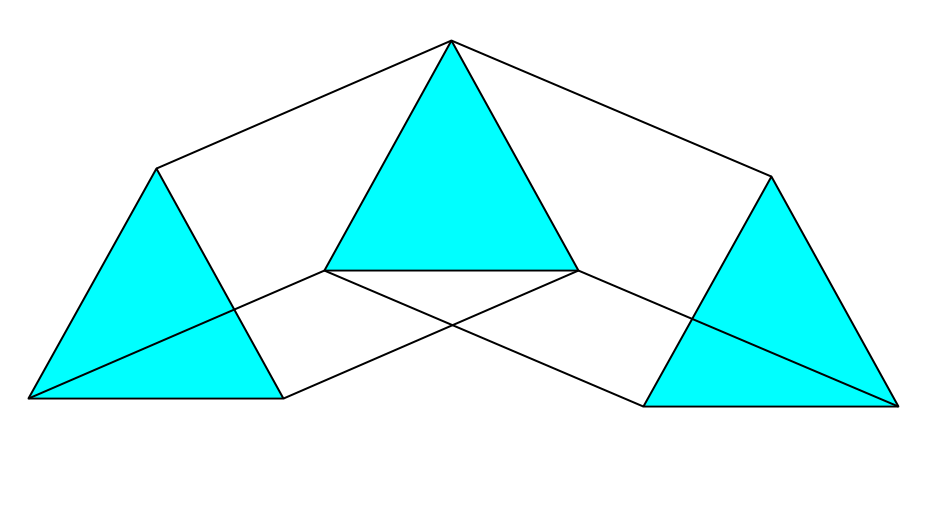
\includegraphics[width=3in]{fig/3DElment.png}
\caption{\small{3D wedge element}} 
\label{fig:3DElment}
\end{figure}

\begin{figure}
\center
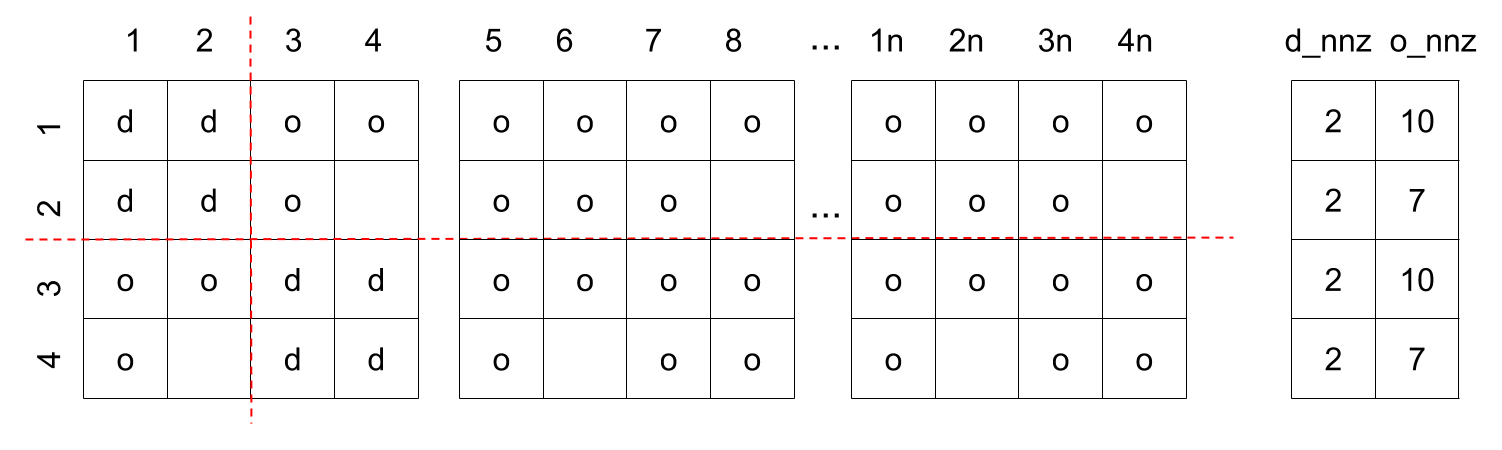
\includegraphics[width=5.5in]{fig/sparseMatrix3D.png}
\caption{\small{Preallocation of the 3D sparse matrix from the 2D mesh in Figure \ref{fig:2d-mesh-psim} }}
\label{fig:sparseMatrix3D}
\end{figure}
%The matrix is created by the PETSc function $MatCreate$. The matrix storage format can be specified by  run-time options (or through corresponding API function). For CSR format, use 
%\begin{samepage}
%\begin{verbatim}
%-mat_type mpiaij
%\end{verbatim}
%\end{samepage}
%and for the block CSR format, use
%\begin{samepage}
%\begin{verbatim}
%-mat_type mpibaij
%-mat_block_size num_dofs_per_node
%\end{verbatim}
%\end{samepage}

Matrix preallocation procedure is called after the matrix is created. The element contribution are added to the matrices by the PETSc function $MatSetValue$, given the value and the location of the row and column to insert the value.  The matrix is assembled by calling the PETSc functions $MatAssemblyBegin$ and $MatAssemblyEnd$.

%\textcolor{blue}{Mark: how matrix is filled-in?}

\subsection{Linear Equation Solvers} \label{sec:linsolver}
Sections 7.3.1 through 7.3.3 presents general overview of the direct method, iterative methods, and the preconditioning methods supported in PETSc. Sections 7.3.4 and 7.3.5 discuss how M3D-C$^1$ solves the problem in 2D and 3D mesh respectively. In 2D, the current code uses direct solving method since the way of using iterative method is unknown and a possible improvement is accounting for the hierarchical block structure of the matrix. In 3D, the iterative method with block Jacobi preconditioned GMRES is used.

\subsubsection{Direct Methods}
This section introduces the background of the direct methods and their usage in PETSc. SuperLU is focused on as the example of the parallel direct solver that can be used through PETSc.

Direct methods use complete or incomplete LU decomposition  (matrix form of Gaussian elimination). In the basic LU decomposition, the matrix in the linear system of equations is factorized into a product of a lower-triangle matrix and a upper-triangle matrix as $A=LU$. The matrix $L$ and $U$ do not maintain the same sparsity as $A$. The incomplete LU decomposition that keeps the sparsity of $A^{k+1}$, $ILU(K)$,  approximates the  original matrix as $A \sim LU$ \cite{saad2003iterative}. When the matrix is symmetric and positive definite,  Cholesky decomposition in the form of $A=LL^T$ is used.

Direct methods In PETSc are generally used as preconditioners to inverse (exactly or approximately) a small sub-matrix in the global matrix, given the fact that direct methods can not be used to solve problems with a  very large size due to the limitation in the parallel scalability.  \textit{\textcolor{blue}{(Fan: PETSc is not designed for a direct sparse linear solver.  There is a build-in   sequential direct solver.  The parallel direct solve is performed by several external solvers interfaced to PETSc \cite{petsc-ug}.  SuperLU is used most  in M3D-$C^1$ as the parallel direct solver. MUMPS \cite{amestoy2000multifrontal} is used occasionally when SuperLU fails.)}}

Parallel sparse direct solvers such as  SuperLU \cite{superlu_ug99} and MUMPS \cite{amestoy2000multifrontal}  are interfaced to PETSc.  In order to reduce the number of additional fill-in's, SuperLU reorders the rows and columns. The reordering takes form as  $P_c^{T} A P_c$, where $P_c$ permutes the columns and   $P_c^{T}$ permutes the rows symmetrically.  Several types of reordering algorithms can be applied by SuperLU, for example, ParMeTiS/MeTiS ordering on $A+A^{T}$,  minimum degree ordering on  $A+A^{T}$ or $AA^T$, and user-specified ordering.  In order to apply the user-specified ordering,  an array that contains the new global  label of each DOF is passed to SuperLU. 

\textit{\textcolor{blue}{(Fan: We tested the reverse Cuthill-McKee ordering from mesh adjacency. But it is not as good as MeTiS ordering used by SuperLu. If we want to get some close result, maybe we can apply a similar mesh-adjacency ordering algorithms with MeTis. The optimal ordering may be unsolvable (NP-hard, see \url{http://en.wikipedia.org/wiki/Band_matrix}). )}}

SuperLu uses a very complex data structure to store the additional fill-in's in the $L$ and $U$ (see Figure 4.1 in \cite{superlu_ug99}). \textit{\textcolor{blue}{(Fan: we may not want to study the very details.)}}

\subsubsection{Iterative Methods}
Iterative methods \cite{barrett1994templates} to solve $A\mathbf{x}=\mathbf{b}$ supported by PETSc include  \cite{petsc-ug}
\begin{itemize}
\item Richardson: the iteration takes form as $\mathbf{x}^{k+1}=\mathbf{x}^k + \omega (b- A\mathbf{x}^k)$.
\item Chebyshev: use $w=2/(\lambda_{min}+\lambda_{max})$ in the Richardson method, where $\lambda_{min}$ and $\lambda_{max}$ are minimum and maximum eigenvalues of $A$.
\item conjugate gradient and  conjugate residual  for symmetric positive definite systems
\item conjugate gradient squared for non-symmetric systems
\item biConjugate gradient of both the original and stabilized versions for non-symmetric systems
\item generalized minimal residual (GMRES) and its variations flexible generalized minimal residual and deflated generalized minimal residual  for general  non-symmetric indefinite system
\item transpose-free quasi-minimal residual for non-symmetric system
\item least squares method 
\end{itemize}

\subsubsection{Preconditioning Methods} \label{sec:precondition}
Preconditioning is a way to convert a linear system into one that is easier solved iteratively \cite{saad2003iterative}.  Define $M$ as the preconditioning matrix. The preconditioned system takes the form
\begin{equation}
M^{-1}A\mathbf{x}=M^{-1}\mathbf{b},
\end{equation} 
or 
\begin{equation}
AM^{-1}\mathbf{u}=\mathbf{b}, \quad \mathbf{x}=M^{-1}\mathbf{u},
\end{equation}
 If $M$ is written in the split form,
\begin{equation}
M=M_{L}M_{R},
\end{equation} 
the split conditioning is of the form
\begin{equation}
M^{-1}_{L}AM^{-1}_{R}\mathbf{u}=M^{-1}_{L}\mathbf{b}, \quad \mathbf{x}=M^{-1}_{R}\mathbf{u}.
\end{equation} 
The preconditioning method are chosen generally based on two aspects \cite{saad2003iterative}. 

Firstly,  the preconditioning matrix $M$ approximates the original matrix adequately for the iterative solving process to converge.  An extreme example to understand this is to consider the direct solver as the preconditioner.  The original matrix is factorized into an lower-triangle matrix and upper-triangle matrix as $A=LU$ (or its variant with row and column permutations). The  inverse of the original matrix $U^{-1}L^{-1}$ is applied directly and no iteration is needed. The incomplete LU decomposition that keeps the sparsity of the original matrix (ILU(0)), approximates the  original matrix as $A \sim LU$. 

Secondly,  the inverse of the preconditioning matrix $M^{-1}$ is cheap to apply. For example, the inverse of $M=LU$ requires solving an upper-triangle  and a lower-triangle linear systems. 

Another aspect to consider is whether it is easy to parallelize the preconditioning method. 

A list of preconditioners that can be combined with the Krylov subspace iterative method  include \cite{petsc-ug}
\begin{itemize}
\item Jacobi: the diagonals of $A$ is used to form the preconditioning matrix $M$.
\item block Jacobi: the diagonal blocks of $A$ is used to form the preconditioning matrix $M$.
\item SOR
\item incomplete or complete cholesky factorization for symmetric positive definite systems
\item incomplete or complete LU 
\item additive schwarz
\item algebraic multigrid
\end{itemize}

%The preconditioning methods can be applied in a very flexible way through PETSc. The preconditioners can be defined by users.  PETSc also support to use preconditioners in a hierarchical way. For example, the  incomplete or complete LU can be used to solve the sub-linear systems in the block Jacobi preconditioned system.  The options to  the preconditioners can be specified by run-time options  \cite{petsc-ug}.

\textcolor{blue}{Mark: I do not want general PETSc reviews. I want to know about specifically what we are doing and why}

\subsubsection{Solving Problems on 2D Mesh: Current Method and Possible Extension} \label{sec:2dproblem}

Currently SuperLu \cite{superlu_ug99}  is used as the direct solver  for the linear systems of equations on 2D meshes. The matrices are quite ill-conditioned and an effective iterative solving method is not found. 

%Since we want to use PETSc as the matrix storage, the direct solvers such as SuperLU \cite{superlu_ug99} and MUMPS \cite{amestoy2000multifrontal} can be used by the following run-time options (or through  API function)
%
% \begin{samepage}
%\begin{verbatim}
%-pc_type lu
%-pc_factor_mat_solver_package superlu_dist # or mumps
%-ksp_type preonly
%\end{verbatim}
%\end{samepage} 

An iterative solving method for 2D problems, if we can find any, can benefit both 2D problems and 3D problems. The 3D problems use a hierarchical-structured preconditioner that corresponding 2D problems are solved first (see the following sub-section for details).

It is possible to find an iterative solving process for the 2D problems if we take advantage of the second-level block structure of the matrix (see Section 
\ref{sec:blockstructure}). The DOFs can be ``split'' into three groups that correspond to the different scalar fields.

For example,  the velocity is decomposed into three scalar fields, $(U,\omega, \chi)$ (Equation \ref{eqn:scalarDecompsition}).   Assume the velocity matrix in the linear system of the equations is $A$. The matrix can be ``split''  into $3\times3$ blocks as
\begin{equation}
\left[\begin{array}{ccc}
A_{UU} & A_{U\omega} & A_{U\chi} \\ 
A_{\omega U} & A_{\omega \omega} & A_{\omega \chi} \\ 
A_{\chi U} & A_{\chi\omega} & A_{\chi\chi} \\ 
\end{array} \right]
\nonumber
\end{equation}

Considering the off-diagonal blocks are small compared with the diagonal blocks \cite{jardin2012multiple},  possible preconditioning methods include \cite{petsc-ug}
\begin{itemize}
\item block Jacobi: there are three diagonal blocks. We can use direct solving method to solve each block. The size of each block is one third of the original system.
\item block Gauss-Seidel:  stronger than block Jacobi since off-diagonal blocks are considered.
\end{itemize}


\textit{ \textcolor{blue}{Fan: PETSc supports to use preconditioner in the ``block'' solvers. The preconditioner type is PETSc PCFIELDSPLIT. There is no guarantee that a specific method will work, but it's worth a try.}}

Besides the velocity equation, the other major linear systems of the equations include the density equation, the pressure equation and the magnetic equation (see Equation \ref{eqn:mhdTimeStepMatrixForm}). The most difficult equation is the velocity equation which contains the most four-order differential operators. 

\textit{ \textcolor{blue}{Fan: If we can find a method to solve the velocity equation iteratively,  it can probably also be applied for other equations.}}

\subsubsection{Solving Problems on 3D Mesh: Current Method and Possible Extension} \label{sec:3Dsolve}
The  linear systems of equations are solved by GMRES with the block Jacobi as the preconditioning method \cite{jardin2012multiple}. The perconditioner  applied is in a hierarchical structure. The overall 3D matrix is approximated by its diagonal blocks  that correspond to  2D cross sections (Figure \ref{fig:3DMatrix}).  Directed solvers are used  to factorize each diagonal block of the matrix.  

\textit{ \textcolor{blue}{Fan: 3D problems is decomposed into a collection of 2D problems. The 2D sub-problems are solved by direct method. If we can find a better way to solve 2D problems, it can be used for 3D problems.}}

\textcolor{blue}{seol -comment from PETSc manual p 173 - the default linear solver for multi-process is GMRES(30) with block Jacobi preconditioning, where there is 1 block per process, and each block is solved with ILU(0). One should experiment to determine alternatives that may be better for various applications. Recall that one can specify the KSP methods and preconditioners at runtime via the options: \emph{-ksp type $<$ksp name$>$ -pc type $<$pc name$>$}. One can also specify a variety of runtime customizations for the solvers.}

The GMRES iterative method is used since it works well for a general non-symmetric  linear system of the equations \cite{saad2003iterative}. 

\textit{ \textcolor{blue}{Fan: we do not know whether the linear system is definite or indefinite. It is difficult to verify analytically.  What we can do is through numerical tests, for example, calculate the eigenvalues of matrix numerically $A+A^{T}$ to see if all eigenvalues are in the same sign. }}
 
The  block-Jacobi preconditioning  method  in 3D problems takes the following facts into consideration (see Section \ref{sec:precondition} for general discussion on preconditioning methods).
\begin{itemize}
\item The 3D matrix is in a cyclic tri-diagonal block way as is illustrated in Figure \ref{fig:3DMatrix}. The diagonal blocks of the matrix is an approximation of the original 3D matrix. 
\item Most of the  ill-conditioning comes from the diagonal blocks that correspond to 2D problems on individual planes. The diagonal blocks are factorized by direct solvers.
\item Jacobi method is naturally  parallelized.
 \end{itemize} 
 
%The preconditioning method  specified  in run-time is the following.
%\begin{samepage}
%\begin{verbatim}
%-pc_type bjacobi
%-pc_bjacobi_blocks number_cross_section
%-sub_pc_type lu
%-sub_pc_factor_mat_solver_package superlu_dist # or mumps
%-sub_ksp_type preonly
%\end{verbatim}
%\end{samepage}

The remaining problems and possible extensions include
\begin{itemize}
\item Direct solvers (full LU decomposition) are used to solve the diagonal blocks that correspond to 2D problems on individual planes. As the problem size on individual planes increases, it is still expensive to apply. An iterative solving process of 2D problems can benefit the iterative solving process of the 3D problem.
\item The diagonal blocks of the matrix do not approximate the 3D matrix adequately. The number of iterations in the GMRES increases as the number of the planes increase (Table \ref{tab:iterNumPlane}). A preconditioner  stronger than block Jacobi can be investigated. For example, the additive Schwarz with overlapped subdomains (there is no overlap in Jacobi method), multi-grid method in the toroidal direction. 
\end{itemize}

 \begin{table}
 \center
  \caption{Number of iterations in block-Jacobi preconditioned GMRES.}  \label{tab:iterNumPlane}
 \begin{tabular}{|l|l|l|l|}
   \hline
   number of planes &  8 &  32 &  64 \\ \hline
  number of iterations & 86 & 458 &  1354  \\ \hline
   \end{tabular}
\end{table}

\subsection{Account for Essential Boundary Condition} 
The essential boundary condition in M3D-$C^1$ constrains a single DOF to be a fixed value. It is applied to the system of equations described by Equation \ref{eqn:sys} directly.
A ``one''  is put at the diagonal of the row  in the matrix $S$ that the corresponding DOF is constrained. The corresponding row of the right-hand-side vector $\mathbf{b}=  D \mathbf{u}^n +\mathbf{f} $ is set to the constrained value. 
%+++++++++++++++++++++++++++++++++++++++++++++++++++++
\section{Data Structure and Algorithms} \label{sec:impl}
%+++++++++++++++++++++++++++++++++++++++++++++++++++++
In the current development,  the 3D linear simulation is used periodically to  check whether non-axis-symmetric instabilities can happen on the 2D nonlinear simulation and the 3D non-linear simulation is used finally to develop instabilities from all three dimensions of the tokamak. Figure \ref{fig:M3DC1LoopNew} depicts the high-level scope of S/W development. 
\begin{itemize} 
\item{[C in Figure \ref{fig:M3DC1LoopNew}]} The new loop starts with the 2D nonlinear simulation (C in Figure \ref{fig:M3DC1LoopNew}) with axis-symmetric solutions.
\item{[E in Figure \ref{fig:M3DC1LoopNew}]} The mesh on the cross section is adapted as needed. 
\item {[F in Figure \ref{fig:M3DC1LoopNew}]} The 3D linear simulation  on the 2D mesh is applied periodically to check whether the non-axis-symmetry can happen.  
\item{[G in Figure \ref{fig:M3DC1LoopNew}]} In case of non-axis-symmetry, the mesh is changed from 2D to 3D and the fields are mapped.
\item{[D in Figure \ref{fig:M3DC1LoopNew}]} The 3D nonlinear simulation loop is applied and instabilities both on the cross section and in the toroidal direction of the tokamak are developed.
\item{[H in Figure \ref{fig:M3DC1LoopNew}]} SCOREC field management library, APF, is used to manage and transfer tensor fields.
\end{itemize}

\begin{figure}[hbt]
\center
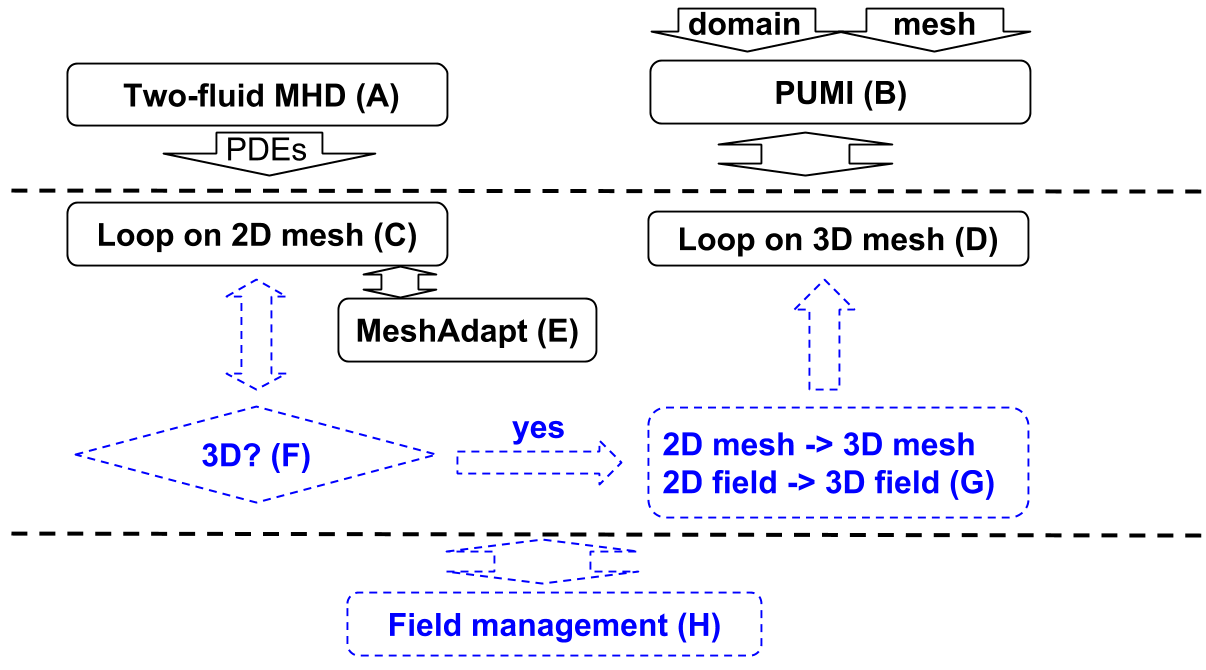
\includegraphics[width=5in]{fig/M3DC1LoopNewSim.png}
\caption{\small{The current S/W status- solid part represents what's completed and dashed part represents what's under development}} 
\label{fig:M3DC1LoopNew}
\end{figure}

The S/W components and features are the following:
\begin{itemize}
\item[-] Input/mesh and geometric information using PUMI. See Sections~\ref{sec:step1} through \ref{sec:step3}.
\item[-] Field/DOF management using APF. See Section ~\ref{sec:step4}.
\item[-] Distributed vector and matrix objects and operations so as to allow M3D-$C^1$ to perform all the operations needed by the matrix solvers. 
\item[-] Access to the distributed matrix storage data structure to assemble the matrices and applying scalability and preconditioning technologies provided in PETSc. .
\item[-] Interpolation-based error indicator to compute mesh size field needed by mesh adaptation. See Section ~\ref{sec:step8}.
\item[-] Anisotropic size-driven mesh adaptation including solution transfer during local mesh modification. See Section ~\ref{sec:step9}.
\end{itemize}

For a complete list of API functions, see Appendix A.

\subsection{Data Structures}
%The API file \emph{m3dc1$\_$scorec.h} provides the following enumerated types for code readibility/writability.

%\begin{verbatim}
%enum m3dc1_coord_system { /*0*/ M3DC1_RZPHI,  // default
%                          /*1*/ M3DC1_XYZ};
%
%enum m3dc1_mesh_ordering { 
%  /*0*/ M3DC1_NO_ADJ=0,  // default - mesh element and DOF ordering use the order from initial mesh 
%                         // generated by mesh generator
%  /*1*/ M3DC1_SERIAL_ADJ, // use adjaceny-based order from the serial mesh; 
%%                          // solver reordering is not used
%  /*2*/ M3DC1_DISTR_ADJ, // use adjaceny-based order from the distributed mesh;
%                         // solver reordering is not used
%  /*3*/ M3DC1_DISTR_ADJ_SOLVER}; // use the adjaceny-based order from distributed mesh and solver
%
%enum m3dc1_field_type { /*0*/ M3DC1_REAL=0,  // real number for field value
%                        /*1*/ M3DC1_COMPLEX}; // complex number for field value
%
%enum m3dc1_matrix_type { /*0*/ M3DC1_SUPERLU=0, 
%                         /*1*/ M3DC1_PETSC, 
%                         /*2*/ M3DC1_MULTIPLY}; 
%
%enum m3dc1_matrix_status { /*0*/ M3DC1_NOT_FIXED=0,
%                           /*2*/ M3DC1_FIXED};
%\end{verbatim}\vspace{-.5cm}\hspace{1cm}

With PUMI, the term \emph{instance} is used to indicate the model data existing on each process. For example, a mesh instance on a process means a pointer to a mesh data structure on the process and all parts on the process are maintained by and accessible through the mesh instance. The term \emph{handle} is used to indicate the pointer to the other data which might exist as multiple objects such as field, part, entity, etc. For example, a mesh entity handle means a pointer to the mesh entity data, and a field handle means a pointer to APF field data created on a mesh instance. When only one data object is needed across the system, the \emph{singleton} design pattern is used, which restricts the instatiation of a class to one object~\cite{designpattern}.

\begin{figure}[hbt]
\center
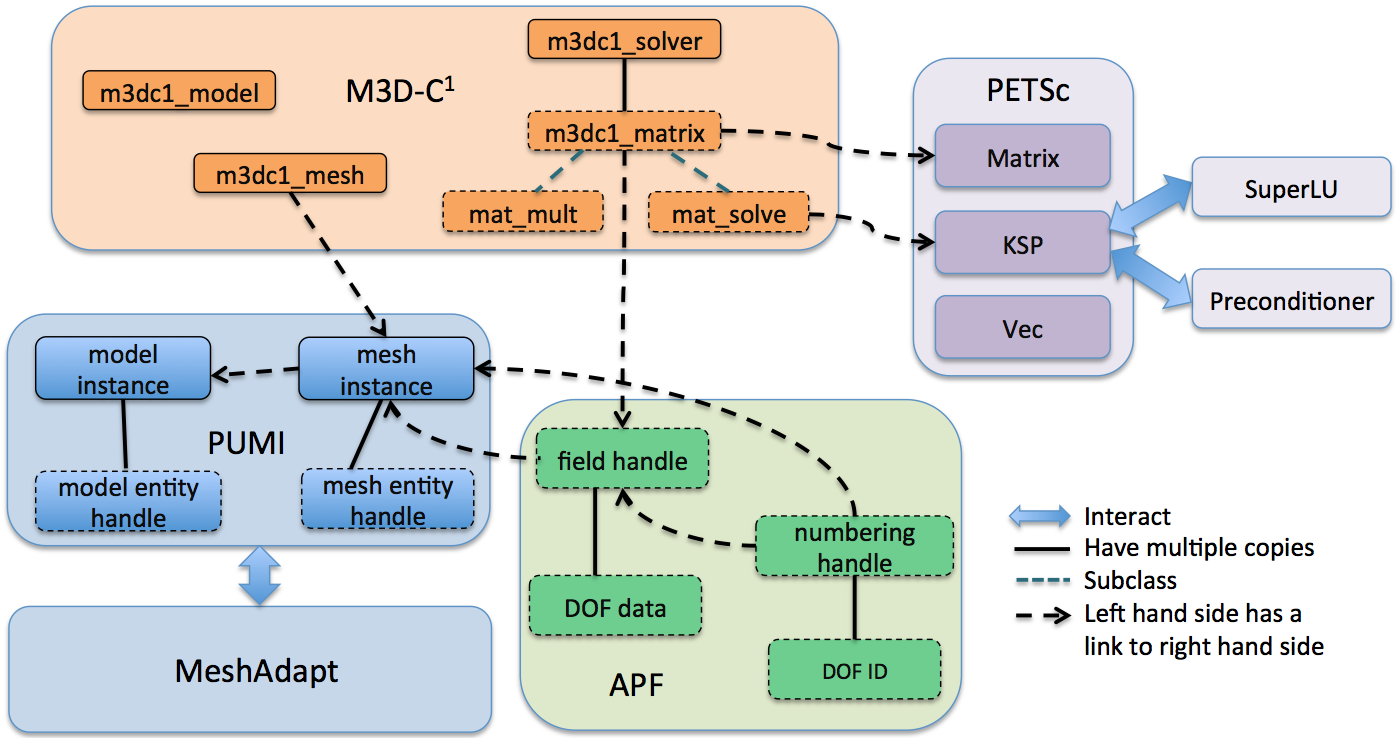
\includegraphics[width=6in]{fig/m3dc1-sw.png}
\caption{\small{Data model in each process: A data drawn with solid rectangle indicates that only one copy of the data exists on a process. A data drawn with solid rectangle indicates that multiple copies of the data exist on a process. A solid line from component $A$ to component $B$ indicates that the component $A$ contains 0 or more component $B$. A dotted arrow from component $A$ to component $B$ indicates that the component $A$ maintains a link to component $B$.}}
\label{fig:m3dc1-datamodel}
\end{figure}

Figure~\ref{fig:m3dc1-datamodel} illustrates a data model in each process. 
\begin{itemize}
\item \emph{m3dc1\_model}: singleton that represents geometric model in M3D-$C^1$. It maintains various information on geometric model which are specific to M3D-$C^1$ so are not maintained in PUMI geometric model instance. For instance, $\varphi$ per process group, the number of planes, etc. The PUMI geometric model can be accessed through PUMI mesh instance so \emph{m3dc1\_model} doesn't maintain the pointer to PUMI geometric model instance.
\item \emph{m3dc1\_mesh}: singleton that represents mesh in M3D-$C^1$. It maintains a pointer to PUMI mesh instance and all the pointers to APF field handle that are created on the mesh. Each APF field handle is uniquely identified by an integer ID which is given by the application at time of field creation.
\item \emph{m3dc1\_matrix}: a class that represents a matrix for M3D-$C^1$. It maintains pointers to PETSc \emph{Mat} object, APF field handle and provide common functions, \emph{create() and fill()} to two subclasses, \emph{mat\_mult} and \emph{mat\_solve}.  The class \emph{mat\_mult} is a matrix for matrix multiplication and the class \emph{mat\_solve} is for equation solver using PETSc \emph{KSP} object. Each matrix is uniquely identified by a integer ID which is given by the application at time of matrix creation.
\item \emph{m3dc1\_solver}: singleton that maintains a map container of matrix id and a corresponding \emph{m3dc1\_matrix} handle. 
\end{itemize}

\subsection{Model/Mesh loading}\label{sec:step1}

Each process loads the geometric model of 2D cross section from a file that describes parameters of the user specified analytic expression that defines a single loop as $R(t)=a_1 + a_2cos\left(t + a_3sin(t)\right)$ and $Z(t)= a_4 + a_5sin(t)$, and the lists of geometric vertex and edges on the wall and vacuum boundaries and parameters of B-splines that define the shape of each edge. The API's related to model are:

\begin{itemize}
\item \emph{m3dc1\_model\_load}: given model file name, each process loads a geometric model that describes the geometry of the 2D cross section of the Tokamak. 
\item \emph{m3dc1\_model\_setnumplane}: given an integer, set the number of planes (process groups)
\item \emph{m3dc1\_model\_setphirange}: given two double values, set the phi range of each plane
\item \emph{m3dc1\_model\_getedge}: get the unique ID's of four model edges of the rectangular domain
\item \emph{m3dc1\_model\_getmincoord}: get the minimum $RZ$ or $XY$ coordinates of the 2D cross section
\item \emph{m3dc1\_model\_getmaxcoord}: get the maximum $RZ$ or $XY$ coordinates of the 2D cross section
\end{itemize}

In 3D with $N$$\times$$P$ processes, the processes are divided to $P$ groups so each process group consists $N$ processes. Then each process group loads 2D mesh which is distributed to $N$ parts and corresponds to a plane. In 2D, the number of process group or plane, $P$, is 1. The API's related to mesh are:
\begin{itemize}
\item \emph{m3dc1\_mesh\_load}: given mesh file name $filename$, $i^{th}$ process of each process group loads mesh entities in $filename-i.sms$, $0$$\le$$i$$\le$$N$$-$$1$. The part boundary links and partition model are managed by PUMI so each process group loads the identical $N$-part mesh.
\item \emph{m3dc1\_mesh\_setcoord}: given an integer describing a coordinate system (enumeration type \emph{M3DC1\_RZPHI} or \emph{M3DC1\_XYZ}), change the coordinates of mesh vertices if different from the current coordinate system. The default coordinate system is \emph{M3DC1\_RZPHI}. 
\item \emph{m3dc1\_mesh\_getnument}: given an integer describing an entity dimension, get the number of \emph{all} entities in the local process.
\item \emph{m3dc1\_mesh\_getnumownent}: given an integer describing an entity dimension, get the number of \emph{owned} entities by the local process.
\item \emph{m3dc1\_mesh\_getnumglobalent}: given an integer describing an entity dimension, get the number of \emph{all} entities in global system. Duplicated entity on part boundaries is counted only once.
\end{itemize}

\subsection{Vertex reordering}\label{sec:step2}

Given an integer describing an ordering option, the API function \emph{m3dc1\_mesh\_setordering} re-orders the mesh vertices in PUMI if needed. The enumeration types for ordering option are the following:
\begin{itemize}
\item \emph{M3DC1\_NO\_ORDER}: default - mesh element and DOF ordering use the order from initial mesh generated by mesh generator.
\item \emph{M3DC1\_ADJ\_ORDER}: mesh element and DOF ordering are based on vertex-element adjaceny. 
\item \emph{M3DC1\_SOLVER\_ORDER}: mesh element and DOF ordering use the order from initial mesh generated by mesh generator. In direct solver step, SuperLU's re-ordering routine is invoked.
\item \emph{M3DC1\_ADJ\_SOLVER\_ORDER}: mesh element and DOF ordering are based on vertex-element adjaceny. In direct solver step, SuperLU's re-ordering routine is invoked.
\end{itemize}

The API to set ordering option is \emph{m3dc1\_mesh\_setordering} so if an input argument is \emph{M3DC1\_DISTR\_ADJ}, it changes the vertex ordering to adjacency-based ordering. This influences both global vertex numbering and DOF numbering.

\subsection{3D mesh construction}\label{sec:step3}
With $N$ $\times$ $P$ processes, where each process group loaded 2D $N$-part mesh representing a plane, the API \emph{m3dc1\_mesh\_build3d()} transform 2D geometric model and mesh to 3D and updated relevant data. The vertex ordering is kept the same so \emph{m3dc1\_mesh\_setordering} doesn't need to be re-called. 

\subsection{Field and numbering}\label{sec:step4}

The API's for field and numbering are:
\begin{itemize}
\item \emph{m3dc1\_field\_create}: given a field ID, field name, the number of field values, and an array for value type(s) (\emph{M3DC1\_COMPLEX} or \emph{M3DC1\_REAL}), and an array for the number of DOF's, it creates a field handle
\item \emph{m3dc1\_field\_delete}: given a field ID, delete a field.
\item \emph{m3dc1\_field\_sync}: given a field ID, synchronizes (unifies) the DOF data on part boundaries
\item \emph{m3dc1\_field\_sum}: given a field ID, sum up the DOF data 
\item \emph{m3dc1\_field\_getnumlocaldof}: given a field id, get the number of local DOF
\item \emph{m3dc1\_field\_getnumowndof}: given a field id, get the number of owned DOF (DOF on owned vertices). The sum of the number of owned DOF on all processes is the number of global DOF.
\item \emph{m3dc1\_field\_getnumglobaldof}: given a field id, get the number of global DOF
\item \emph{m3dc1\_field\_getlocaldofid}: given a field ID, get the local DOF ID range (first local DOF ID and the last local DOF ID+1)
\item \emph{m3dc1\_field\_getowndofid}: given a field ID, get the global, owned DOF ID range (first global DOF ID and the last global DOF ID+1 owned by the local process)
\item \emph{m3dc1\_field\_getglobaldofid}: given a field ID, get the global DOF ID range (first DOF ID and the last DOF ID+1)
\end{itemize}

The entity-level API's for DOF data and numbering are:
\begin{itemize}
\item \emph{m3dc1\_ent\_getlocaldofid}: given entity dimension, local entity ID, and field ID, get the local DOF ID range (first local DOF ID and the last local DOF ID+1)
\item \emph{m3dc1\_ent\_getglobaldofid}: given entity dimension, local entity ID, and field ID, get the global DOF ID range (first global DOF ID and the last global DOF ID+1)
\item \emph{m3dc1\_ent\_getnumdof}: given entity dimension, local entity ID, and field ID, get the number of DOF
\item \emph{m3dc1\_ent\_setdofdata}: given entity dimension, local entity ID, and field ID, set the DOF data
\item \emph{m3dc1\_ent\_getdofdata}: given entity dimension, local entity ID, and field ID, set the number of DOF and DOF data
\end{itemize}

\subsection{Matrix and solver} \label{sec:step7}
\begin{itemize}
\item \emph{m3dc1\_matrix\_create}: given a matrix id, matrix type (\emph{MATRIX\_MULT} or \emph{MATRIX\_SOLVE}), scalar type, and field id, it creates a matrix
\item \emph{m3dc1\_matrix\_freeze}: given a matrix id, freeze the matrix (no matrix update is allowed after this).
\item \emph{m3dc1\_matrix\_delete}:  given a matrix id, delete the matrix

\item \emph{m3dc1\_matrix\_insert}: given a matrix id, row number, column number, scalar type and one or more double values,  insert the value to the matrix[row, column]
\item \emph{m3dc1\_matrix\_add}: given a matrix id, row number, column number, scalar type and one or more double values,  add the value to matrix[row, column]
\item \emph{m3dc1\_matrix\_setbc}: given a matrix ID and a row number, it specifies the row that the corresponding DOF is constrained. During matrix assembly stage, the rows that are specified by $ m3dc1\_matrix\_setdbc$ are zeroed and put ``ones'' at the diagonal.
\item \emph{m3dc1\_matrix\_solve}: given a matrix ID and field ID, it solves
\item \emph{m3dc1\_matrix\_multiply}: given a matrix ID and field ID, it multiplies
\item \emph{m3dc1\_matrix\_write}: matrix file I/O. Not supported.
\end{itemize}

%+++++++++++++++++++++++++++++++++++++++++++++++++++++
\section{Parallelization} \label{sec:issues}
%+++++++++++++++++++++++++++++++++++++++++++++++++++++

%+++++++++++++++++++++++++++++++++++++++++++++++++++++
\subsection{Options for simulation mode switch in run-time}

In terms of the simulation mode switch in run-time, there are three options.
\begin{itemize} 
\item{Option 1.} From 3D axis-symmetric to full 3D: it requires transforming 2D mesh with real tensor fields to 3D mesh with real tensor fields. 
\item{Option 2.} From 3D analytic to full 3D: it requires transforming 2D mesh with complex tensor fields to 3D mesh with real tensor fields.
\item{Option 3.} From 3D axis-symmetric to 3D analytic: it requires transforming 2D mesh with real tensor fields to 2D mesh with complex tensor fields. 
\end{itemize} 

Since PPPL and SCOREC agreed to support Option 1 and 2, herein we only discuss issues relevant to Option 1 and Option 2. \textcolor{blue}{Do we need to support Option 3?}

%+++++++++++++++++++++++++++++++++++++++++++++++++++++
\subsection{API's to support field management through APF}

Given the dimension of the field, the type of arithmetic and the definition of the $C^1$ elements, the field data are created and maintained in SCOREC field management library, APF.  The type of arithmetic indicates whether the real or complex number is used. The definition of the $C^1$ elements describes the number of DOFs attached to the mesh vertex, and the method to evaluate the shape function associated with each DOF. APF provides manipulation of DOF data and numbering through well-defined APIs.

%+++++++++++++++++++++++++++++++++++++++++++++++++++++
\subsection{Accessing mesh entities in PUMI via pointer}
M3D-$C^1$ accesses the mesh entities based on mesh dimension and entity id (inherited from the previous implementation). Since entity ID is not maintained at the PUMI level for efficiency issue, accessing mesh entity through ID requires substantial overhead such as duplicate mesh copy sorted in global entity id order and maintaining mesh copy and global ID over mesh modification. If M3D-$C^1$ needs to access mesh entities directly, the ideal approach is using \emph{opaque} type entity pointer instead of global entity id. The coordination between PPPL and SCOREC is needed to improve the Fortran and C++ interactions over the mesh entity access to get rid of global entity id.

%+++++++++++++++++++++++++++++++++++++++++++++++++++++
\subsection{Memory management for field - M3D-$C^1$ vs. APF}

Based on the number of DOFs per vertex, APF allocates contiguous memory for storing all DOFs and provides efficient manipulation over DOFs including numbering, global data and ID synchronization, automatic DOF data migration along the mesh migration and modification, binary file I/O, etc. 

In the previous development that didn't use APF for field management, the SCOREC tool provided only DOF numbering per vertex and the rest of field management such as storage and manipulation was performed out of SCOREC tools. For seamless and efficient management of mesh and field data defined over mesh, keeping field data storage in the APF is desirable. 

If field data is stored and maintained by APF, M3D-$C^1$ can set/get field data only through API's, \emph{m3dc1\_ent\_setdofdata} and \emph{m3dc1\_ent\_getdofdata}. SCOREC forks should clearly understand the scope of involved changes in the M3D-$C^1$ Fortran code to carry out this task.

%+++++++++++++++++++++++++++++++++++++++++++++++++++++
\subsection{Dynamic scalar type change in M3D-$C^1$}

APF can support both REAL and COMPLEX without recompiling the library. However, the current M3D-$C^1$ Fortran library should be re-compiled with compilation flag (\#ifdef USECOMPLEX) to switch between REAL and COMPLEX number for scalar type. 

%+++++++++++++++++++++++++++++++++++++++++++++++++++++
\subsection{Field mapping between different modes }
\begin{itemize}
\item In mode switch from 3D axis-symmetric to full 3D, the 3D axis-symmetric solution is invariant in the toroidal direction ($\partial/\partial \varphi =0$).
Given a 3D axis-symmetric field $U$ (defined on 2D mesh),  DOFs corresponding to $U$, $U_{,R}$, $U_{,Z}$, $U_{,RR}$, $U_{,RZ}$, $U_{,ZZ}$ in the 3D mesh are assigned the same values as the original 2D mesh. DOFs corresponding to $ U_{,\varphi}$, $U_{,R\varphi}$, $U_{,Z\varphi}$, $U_{,RR\varphi}$, $U_{,RZ\varphi}$, $U_{,ZZ\varphi}$ are assigned to zero since the 3D field is still axis-symmetric and there is no variation in the $\varphi$ direction. For each vertex, the number of DOFs is changed from 6 to 12, thus for the new 12 DOFs, the existing 6 DOFs are copied and the rest of 6 DOFs is set to 0.

\item In mode switch from 3D analytic to full 3D, the 3D analytic solution varies in the toroidal direction as $\sim e^{i\cdot n\varphi}$. The 3D analytic solution (defined on 2D mesh) as
\begin{equation}
\left[  Re(R,Z)+i\cdot Img(R,Z)  \right] e^{i\cdot n\varphi}
 \end{equation} 
  where $Re(R,Z)$ and $Img(R,Z)$ are the real part and imaginary  part of the solution. We need to construct a 3D field from this information.
\end{itemize}

%+++++++++++++++++++++++++++++++++++++++++++++++++++++
\subsection{Different number of processes needed in different modes}
When the simulation domain is changed from \emph{one} 2D plane to 3D mesh constructed with $P$ planes, a 2D plane distributed in $N$ processes is copied to the rest $P-1$ planes requiring $N$ $\times$ $P$ processes total. In terms of different number of process requirement, there are four options.
\begin{itemize}
\item{Option 1.} In 2D, the simulation runs with $N$ processes then the number of processes is increased to $N$ $\times$ $P$ to construct 3D mesh. This is the most straightforward method but more technical investigation is needed to know how it can be achieved since parallel system does not allow that to occur within a single run. 
\item{Option 2.} The simulation runs with $N$ $\times$ $P$ processes. The first process group (process $0$ to process $N-1$) loads 2D mesh and does simulation while the rest $(P-1)$ process groups are idle. When the 3D simulation starts, the 2D mesh in the first process group is copied to the rest $(P-1)$ process process groups then 3D mesh is constructed (See Figure~\ref{fig:wedgePlane}). This option is relatively straightforward but expensive.
\item{Option 3.} The simulation runs with $N$ $\times$ $P$ processes. In 2D, $N$ part mesh is distributed to $N$ $\times$ $P$ processes keeping all the processes busy to run 2D simulation. After 2D simulation is over, 2D mesh distributed on $N$ $\times$ $P$ processes is merged to $N$ processes and the 2D mesh is copied to the rest $N$ $\times$ $(P-1)$ processes to construct the 3D mesh. 
\item{Option 4.} The simulation runs with $N$ processes. In 2D, $N$ part mesh is distributed to $N$ processes keeping all the processes busy to run 2D simulation. After 2D simulation is over, 2D mesh is merged to $N/P$ processes and the same 2D mesh is copied to the rest $N-N/P$ processes to construct 3D mesh.  
\end{itemize}

\begin{figure}
\center
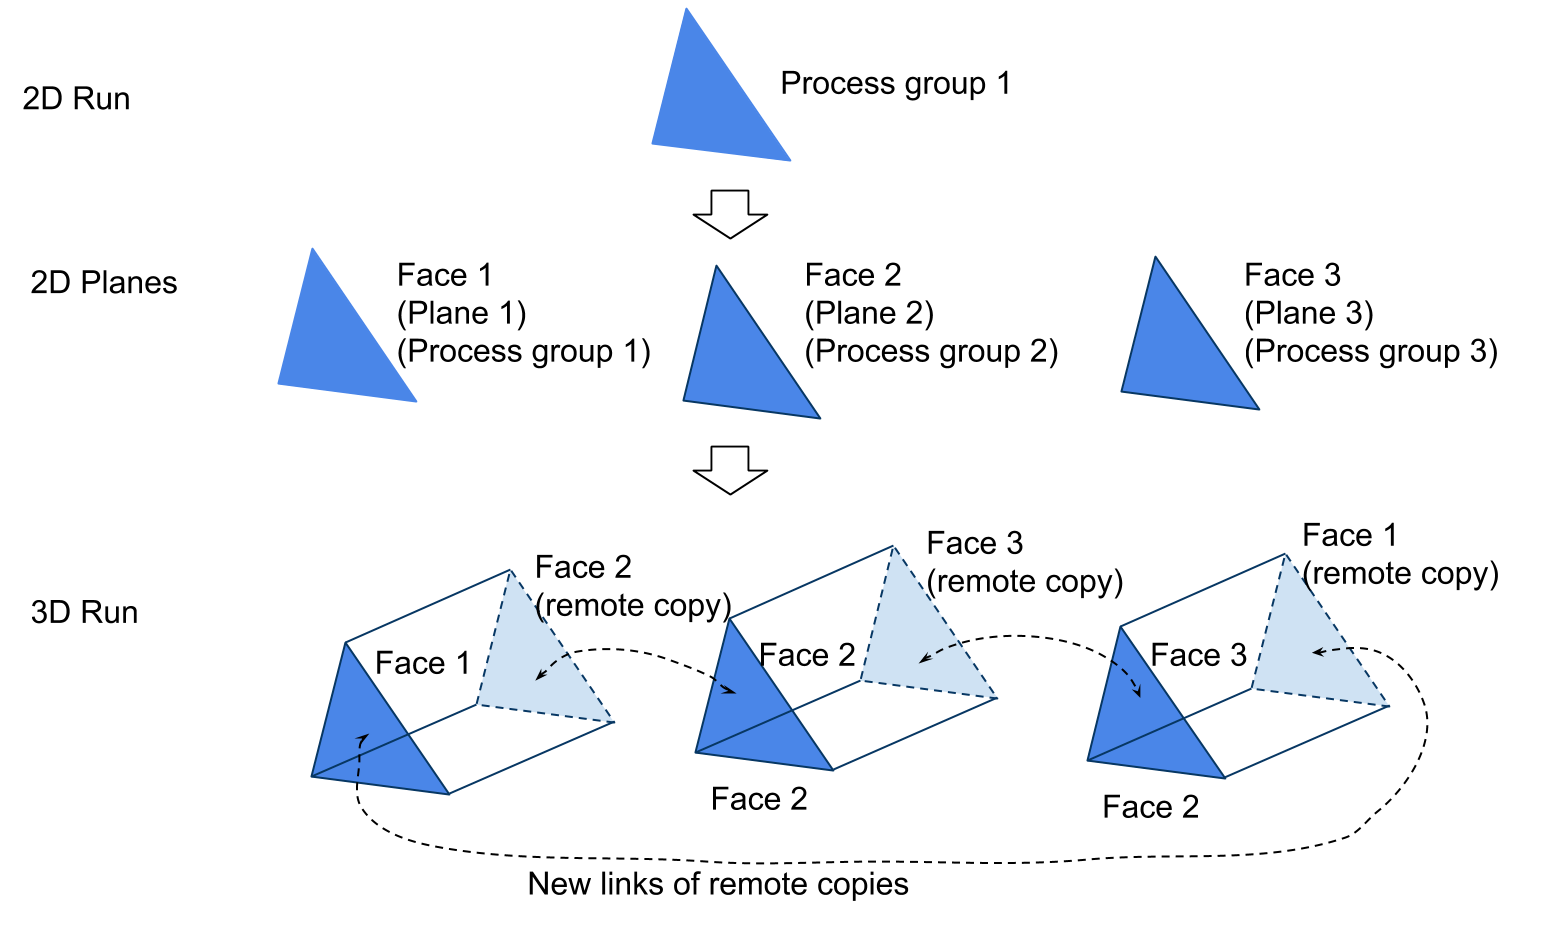
\includegraphics[width=0.8\textwidth]{fig/wedgePlane.png}
\caption{\small{Option 2: idling processes in 2D simulation.}} 
\label{fig:wedgePlane}
\end{figure}

Figure~\ref{fig:wedgePlane2} illustrates an example run of Option 4 running on 6 processes. First, a 2D plane is distributed 6 parts to run 2D simulation. Then in order to construct 3D mesh, 6 part mesh is merged to the first 2 processes and copied to the remaining 4 processes resulting in three 2D planes on 6 processes such that process 1 holds part 1, 2 and 3, process 2 holds part 4, 5, and 6, process 3 holds part 1, 2, and 3, and process 4 holds part 4, 5 and 6, and so on.

\begin{figure}
\center
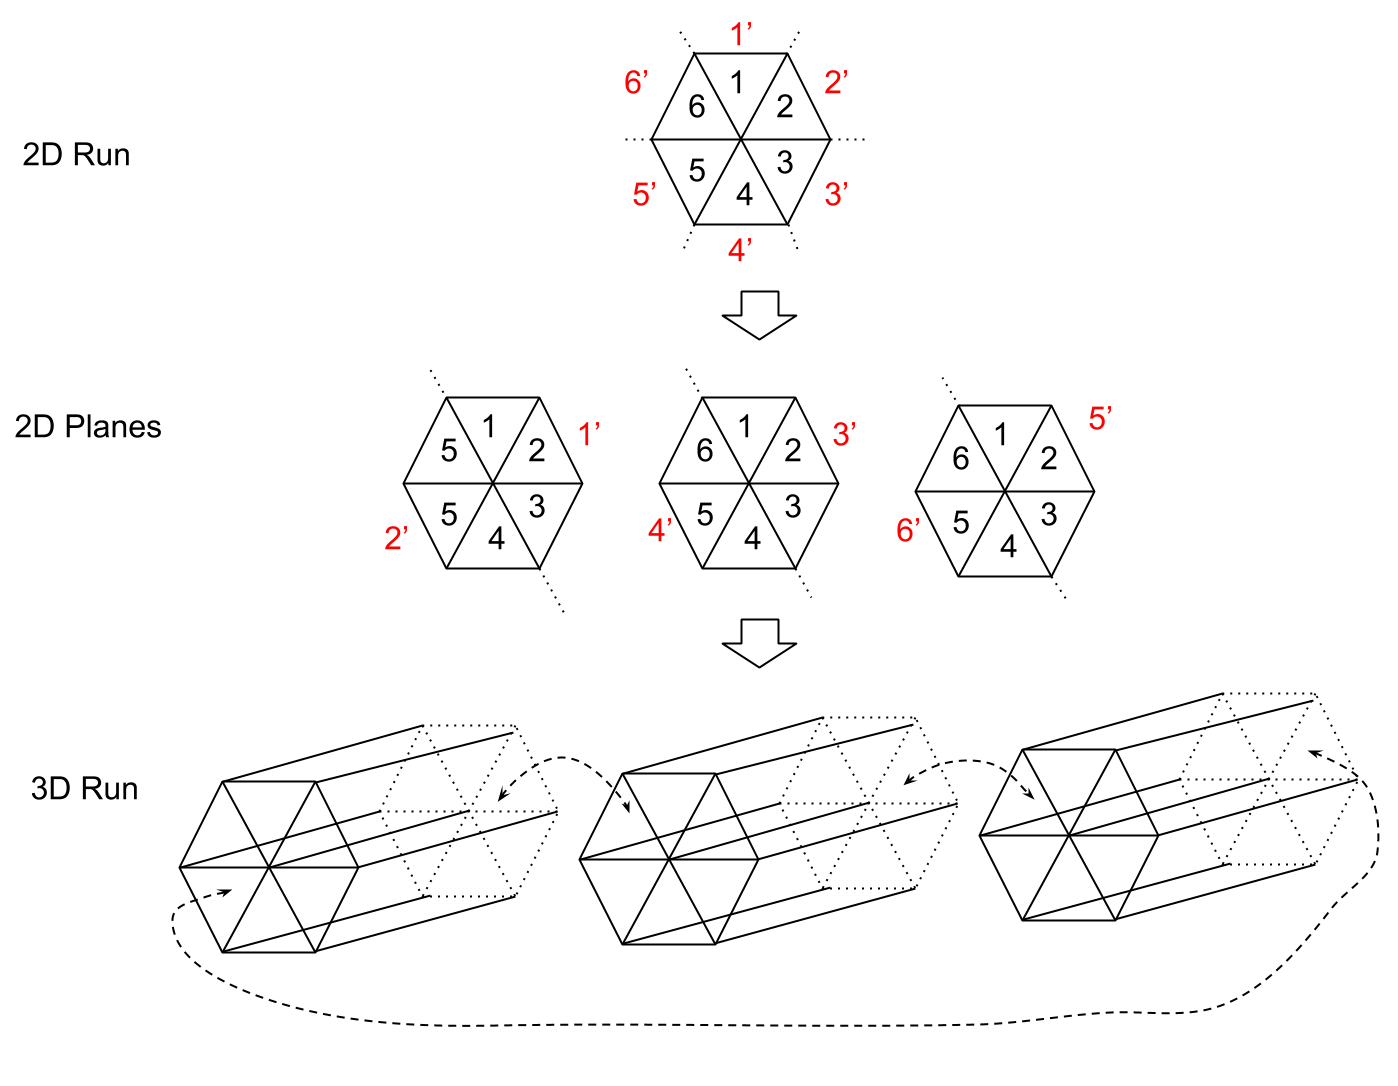
\includegraphics[width=0.8\textwidth]{fig/wedgePlane2.png}
\caption{\small{Option 4: multiple parts on a single process. Each process holds 3 parts on the 3D mesh.}} 
\label{fig:wedgePlane2}
\end{figure}

Assuming the option 1 is not technically feasible, Option 3 and 4 are the most inexpensive method in terms of keeping all the processes busy and minimizing simulation time in 2D. PUMI supports all the tools needed to merge/re-distribute the mesh and related data. However, until the trade-off between gain and loss due to dynamic mesh merging and re-partitioning is fully studied, Option 2 will be taken as an approach.  

%+++++++++++++++++++++++++++++++++++++++++++++++++++++
\subsection{In-memory adaptive workflow}

In terms of data transfer and sharing between libraries, using file I/O in pre-defined format is the easiest to implement, but the least efficient due to the file I/O bottleneck. The existing code uses file I/O between mesh adaptation on the cross section and continued simulation on the adapted mesh. 
For efficiency, in-memory adaptive workflow needs to be developed by linking mesh adaptation and continued simulation with a well-defined set of API instead of file-based interactions.

%+++++++++++++++++++++++++++++++++++++++++++++++++++++
\subsection{Error estimation}
Improved 2D error estimations are desired. Examination of the options for 2D to 3D with comparison, given in the beginning of Section 4, needs to be carried out. An error indicator to select the number of desired planes in the 3D mesh is needed.

%+++++++++++++++++++++++++++++++++++++++++++++++++++++
\section{Comparing Run-Time of 3D Problems} \label{sec:issues}
\subsection{A 3D test on Greene and Edison}
The running time of M3D-$C^1$ using the old and new implementation of SCOREC libraries are compared. The difference in running time comes from the different implementation of matrix. In the old version, we implemented our data structure of matrix, and parallel assembly of the matrix. The assembled matrix is either passed to PETSc or SuperLu to solve the system of equations, or used to multiply a vector.  In the new version, we use PETSc directly as the underlying implementation of matrix and let PETSc handle the parallel assembly of the matrix.

Two types of matrices are used in M3D-$C^1$. The first type of matrices are used only to perform matrix-vector production.  The matrix values at mesh part boundary need not to be complete. This type of matrices are not assembled parallellly. The second type of matrices is used to form the system of equations that requires more general operations such as applying preconditioning method.   Matrices of this type require complete values at mesh part boundary and are assembled parallellly.

Table \ref{tab:3DGreene} and Table \ref{tab:3DEdison} compare the running time using the old and new implementation of SCOREC libraries. The columns in the tables are explained as below.
\begin{itemize}
\item calculate element: the element contribution on the local mesh to the matrices are calculated and added to the matrices.
\item  finalize multiply matrix: the matrix to multiply a vector is finalized. The matrix values at mesh part boundary are incomplete and parallel assembly is not performed.
\item finalize solve matrix: the matrix to form the system of equations that requires more general operations is finalized. The matrix values at mesh part boundary are complete. Parallel assembly is performed.
\item solve: the  system of equations is solved.
\item other: it includes all the other routines not listed above such as calculating secondary variables.
\item total: it includes the total time to run a time step.
\end{itemize}
 \begin{table}
 \center
  \caption{A 3D test with 4 planes, 16 processes, 1034 nodes per plane on Greene}  \label{tab:3DGreene}
 \begin{tabular}{|l|l|l|l|l|l|l|}
   \hline
    &  calculate element & finalize multiply matrix & finalize solve matrix & solve & other & total  \\ \hline
  old  & 250.8 & 44.4 &  6.2 & 23.9 & 37.8 & 363.1  \\ \hline
  new  & 199.8& 3.4 &  15.3 & 20.2 & 31.1 & 269.8  \\ \hline
   \end{tabular}
\end{table}

 \begin{table}
 \center
  \caption{A 3D test with 8 planes, 196 processes, 1034 nodes per plane on Edison}  \label{tab:3DEdison}
 \begin{tabular}{|l|l|l|l|l|l|l|}
   \hline
    &  calculate element & finalize multiply matrix & finalize solve matrix & solve & other & total  \\ \hline
  old  &143.5 & 6.0 &  0.5 & 6.6 & 21.2 & 177.8  \\ \hline
  new  & 138.9& 7.2 &  267.1 & 5.4 & 21.4 & 440.0  \\ \hline
   \end{tabular}
\end{table}

Table \ref{tab:3DGreene} compares the running time on Greene (PPPL computing cluster) with 16 processes. It shows $20\%$ improvement in calculating element, and $92\%$ improvement in finalizing multiply matrix. The stage of finalizing solve matrix is slower by $15\%$. The overall running time is reduced by $26\%$ for the test.

Table \ref{tab:3DEdison} compares the running time on NERSC Edison with 196 processes. The new implementation runs slower than the old implementation. The step of finalizing solve matrix dominates the running time. We will need a more efficient way to assemble  the matrix parallelly.

\subsection{Analysis of result}
We show improvements in the step of calculating element by using PETSc directly as underlying matrix implementation, but PETSc does not perform well in parallel assembly.

The reason that PETSc does not perform well in parallel assembly is that it is not mesh-aware enough. It does not know ahead which values will be generated at mesh part boundary and which processes these values will be sent. PETSc assumes only a small amount of matrix values are generated ``owned'' by other processes. It requires extra memory and communication to store matrix values owned by other processes. However, $50\%$ of matrix values generated belong to other processes in 3D problem. A wedge element is constructed by connecting the triangle on current plane and the triangle on the next plane. The values associated with the triangle on the next plane belong to other processes.

In our old implementation,  we know ahead  which values will be generated at mesh part boundary and which processes these values will be sent. The matrix is assembled parallely by performing the neighborhood communication between processes based on mesh partition \cite{sahni2009strong,ovcharenko2012neighborhood}.

\subsection{Matrix assembly}
We implemented the procedure of parallel matrix assembly. The algorithm is still based on the neighborhood communication between processes \cite{sahni2009strong,ovcharenko2012neighborhood}.  We will use a sequential matrix to store the values belonged to other processes and the matrix values are communicated based on mesh partition.  The algorithm will improve the step of  finalizing solve matrix in Table \ref{tab:3DEdison}. It will potentially improve the step of calculating element since PETSc will not ``see'' values belong to other processes at this step. 
%+++++++++++++++++++++++++++++++++++++++++++++++++++++



\bibliographystyle{ieeetr}
\bibliography{reference}

\clearpage
\appendix
%%%%%%%%%%%%%%%%%%%%%%%%%%%%%%%
\section{API Functions}
%%%%%%%%%%%%%%%%%%%%%%%%%%%%%%%
The section describes the specification of API functions provided to the M3D-C1 Fortran driver. The function prototypes are declared in the file \texttt{m3dc1$\_$scorec.h}. Throughout this section, unless specified, mesh entities and DOF's are specified by a local ID. A word ``\emph{global}'' in a function name indicates that the function involves global operation or global data.

%%%%%%%%%%%%%%%%%%%%%%%%%%%%%%%
\subsection{Initialization and finalization}
%%%%%%%%%%%%%%%%%%%%%%%%%%%%%%%
The functions initialize/finalize the PUMI operations.

\begin{verbatim}
// fortran name: m3dc1_domain_init
int m3dc1_scorec_init();
\end{verbatim}\vspace{-.5cm}\hspace{1cm}
Initialize the PUMI service for distributed model and mesh infrastructure. Note that MPI should be initialized prior to this function.

\begin{verbatim}
// fortran name: m3dc1_domain_finalize
int m3dc1_scorec_finalize();
\end{verbatim}\vspace{-.5cm}\hspace{1cm}
Finalize the PUMI service and clears all PUMI related data. Note that MPI finalization should follow.

%%%%%%%%%%%%%%%%%%%%%%%%%%%%%%%
\subsection{Plane}
%%%%%%%%%%%%%%%%%%%%%%%%%%%%%%%

\begin{verbatim}
int m3dc1_plane_setphi(
    int*  /* in */  planeid, 
    double*   /* in */  phi);
\end{verbatim}\vspace{-.5cm}\hspace{1cm}
Given a plane ID and a double, set the phi value of the plane.

\begin{verbatim}
int m3dc1_plane_getphi(
    int*  /* in */  planeid, 
    double*  /* out */  phi);
\end{verbatim}\vspace{-.5cm}\hspace{1cm}
Given a plane ID, return the value of phi of the plane.

%%%%%%%%%%%%%%%%%%%%%%%%%%%%%%%
\subsection{Geometric model}
%%%%%%%%%%%%%%%%%%%%%%%%%%%%%%%

\begin{verbatim}
int m3dc1_model_load (char*  /* in */  model_file);
\end{verbatim}\vspace{-.5cm}\hspace{1cm}
Load a geometric model from a model file that describes the geometry of the 2D cross section of the Tokamak. The file can contain
\begin{itemize}
\item parameters of the user specified analytic expression that defines a single loop as $R(t)=a_1 + a_2cos\left(t + a_3sin(t)\right)$ and $Z(t)= a_4 + a_5sin(t)$.
\item lists of geometric vertex and edges on the wall and vacuum boundaries and parameters of B-splines that define the shape of each edge.
\end{itemize}

\begin{verbatim}
int m3dc1_model_setnumplane (int*  /* in */  num_plane);
\end{verbatim}\vspace{-.5cm}\hspace{1cm}
Given an integer \textit{num$\_$plane}, set the number of planes in 3D. For 2D, the number of plane is 1.

\begin{verbatim}
int m3dc1_model_getnumplane (int*  /* out */  num_plane);
\end{verbatim}\vspace{-.5cm}\hspace{1cm}
Return the number of planes. For 2D, the number of plane is 1.

\begin{verbatim}
int m3dc1_model_getplaneid (int*  /* out */  plane_id);
\end{verbatim}\vspace{-.5cm}\hspace{1cm}
Return the plane ID where the local process belongs. The plane ID starts from 0.

\begin{verbatim}
int m3dc1_model_getedge (
    int*  /* out */  left_edge, 
    int*  /* out */  right_edge,
    int*  /* out */  bottom_edge, 
    int*  /* out */  top_edge); 
\end{verbatim}\vspace{-.5cm}\hspace{1cm}
Return the four model edges of the rectangular domain.

\begin{verbatim}
int m3dc1_model_getmincoord (
    double*  /* out */  x_min, 
    double*  /* out */  y_min);
\end{verbatim}\vspace{-.5cm}\hspace{1cm}
Return the minimum coordinate of the 2D cross section.
	      \textit{x\_min} is the minimum horizontal coordinate value. 
	      \textit{z\_min} is the minimum vertical coordinate value.

\begin{verbatim}
int m3dc1_model_getmaxcoord (
    double*  /* out */  x_max, 
    double*  /* out */  y_max);
\end{verbatim}\vspace{-.5cm}\hspace{1cm}
Return the maximum coordinate of the 2D  cross section. 
          \textit{x\_max} is the maximum horizontal coordinate value. 
          \textit{Y\_max} is the maximum vertical coordinate value.

\begin{verbatim}
int m3dc1_model_print();
\end{verbatim}\vspace{-.5cm}\hspace{1cm}
Display the model information.

%%%%%%%%%%%%%%%%%%%%%%%%%%%%%%%
\subsection{Mesh}
%%%%%%%%%%%%%%%%%%%%%%%%%%%%%%%
When a mesh is distributed in parallel, a mesh entity can be uniquely identified in two ways: (i) an entity dimension and a global entity ID, or (ii) an entity dimension, a process rank and a local entity ID. The entity dimension is 0 for vertex, 1 for edge, 2 for face and 3 for region. For M3D-$C^1$, each mesh vertex has a $node$ serving as DOF holder. A mesh entity of highest dimension (face in 2D and region in 3D) is termed $element$. 

For a distributed mesh on multiple parts, mesh entities not on part boundaries are termed \textit{internal entity} and duplicated mesh entities along part boundaries are termed \textit{part boundary entity}. Among multiple copies of a part boundary entity, one entity is designated to be an \textit{owner copy} and is in charge of updating the rest of copies. The rest of entity copies are termed \textit{non-owned part boundary entity}. For a part boundary entity, duplicate \textit{off-part} copies are termed \textit{remote copy}. All internal entities are owner copies.

To avoid communications between the parts, it is beneficial to support the ability to have a copy of $non$-part boundary entities on other part, referred as $ghosting$. A \textit{ghost copy} is a read-only, duplicated, off-part internal entity copy including global ID, tag data, and field data. Similar to the ownership of part boundary entities, the original owner copy is designated as \emph{owner} of all \textit{ghost copies}.

\begin{verbatim}
int m3dc1_mesh_load (char*  /* in */  mesh_file);
\end{verbatim}\vspace{-.5cm}\hspace{1cm}
Load a mesh from mesh file(s).

\begin{verbatim}
int m3dc1_mesh_build3d ();
\end{verbatim}\vspace{-.5cm}\hspace{1cm}
Construct 3D mesh from multiple 2D planes where each plane is loaded with 2D mesh. 

\begin{verbatim}
// fortran name: m3dc1_ghost_load
int m3dc1_ghost_create (int*  /* in */  n);
\end{verbatim}\vspace{-.5cm}\hspace{1cm}
Given an integer \textit{n}, create $n$ ghost layer(s) in the mesh.

To perform ghosting with $d$-dimensional mesh, PUMI requires four input arguments: (i) ghost type $g$ (0$<$$g$$\le$$d$) for entity type to be ghosted, (ii) bridge type $b$ ($b$ $<$ $g$ and $b$$\ne$$g$),  (iii) the number of ghost layers $n$ measured from part boundary up to the number with which whole part can be ghosted, (iv) a boolean flag to indicate whether to include non-owned bridge entities or not in ghosting candidate computation. If true, all part boundary entities of bridge dimension are considered to construct ghost layer(s). If false, only $owner$  part boundary entities of bridge dimension are considered. 

In case of ghosting procedure in M3D-$C^1$, the bridge dimension, the ghost dimension, and the flag are, respectively, set to $d$-$1$, $d$, and $true$.

\begin{verbatim}
int m3dc1_ghost_delete ();
\end{verbatim}\vspace{-.5cm}\hspace{1cm}
Delete the ghost layer(s).

\begin{verbatim}
int m3dc1_mesh_getnumglobalent (
    int*  /* in*/  ent_dim, 
    int*  /* out */  num_global_ent);
\end{verbatim}\vspace{-.5cm}\hspace{1cm}
Given an entity dimension (0-3), return the number of $unique$ entities on all processes. \textit{Non-owned} part boundary entities and \textit{ghost copies} are not counted.

\begin{verbatim}
//fortran name: m3dc1_mesh_getnument
int m3dc1_mesh_getnumlocalent (
    int*  /* in*/  ent_dim, 
    int*  /* out */  num_local_ent);
\end{verbatim}\vspace{-.5cm}\hspace{1cm}
Given an entity dimension (0-3), return the number of entities on local process. 

\begin{verbatim}
int m3dc1_mesh_getnumownent (
    int*  /* in*/  ent_dim, 
    int*  /* out */  num_own_ent);
\end{verbatim}\vspace{-.5cm}\hspace{1cm}
Given an entity dimension (0-3), return the number of owner copies on local process.

\begin{verbatim}
int m3dc1_mesh_getnumghostent (
    int*  /* in*/  ent_dim, 
    int*  /* out */  num_ghost_ent);
\end{verbatim}\vspace{-.5cm}\hspace{1cm}
Given an entity dimension (0-3), return the number of ghost copies on local process.

\textcolor{red}{Added to support PIC}

\begin{verbatim}
int m3dc1_mesh_search (
    int*  /* in */   initial_simplex, 
    double*  /* in */  final_position, 
    int*  /* out */  final_simplex);
\end{verbatim}\vspace{-.5cm}\hspace{1cm}
\textcolor{red}{\textit{Kaushik will provide the specification}}

\begin{verbatim}
int m3dc1_mesh_write (
    char*  /* in */  filename, 
    int*  /* in */  option);
\end{verbatim}\vspace{-.5cm}\hspace{1cm}
Write the mesh in file(s). Set the option to 0 for Paraview format (.vtk) and 1 for PUMI format (.smb).

%%%%%%%%%%%%%%%%%%%%%%%%%%%%%%%
\subsection{Mesh Adaptation and Solution Transfer}
%%%%%%%%%%%%%%%%%%%%%%%%%%%%%%%

\textcolor{red}{\textit{Mesh adaptation is not supported for ghosted mesh in the current version}}

\begin{verbatim}
int adapt_by_field (
    FieldID  /* in */  field_id, 
    double*  /* in */  psi0,  
    double*  /* in */  psil); 
\end{verbatim}\vspace{-.5cm}\hspace{1cm}
The function adapts the mesh by the analytic size field defined in terms of  the solution field. The parameters in the analytic expression are defined in the file sizefieldParam. \textit{field$\_$id} is is the solution field. \textit{psi0} and \textit{psil} are two parameters to normalize the field value. The normalized field value is $\bar{psi} = (psi - psi0)/(psil - psi0)$.

\begin{verbatim}
int set_adapt_p (double*  /* in */  pp);
\end{verbatim}\vspace{-.5cm}\hspace{1cm}

\begin{verbatim}
int adapt_by_error_field (
    double*  /* in */  errorField, 
    double*  /* in */  errorAimed, 
    int*  /* in */  max_node, 
    int*  /* in */  option); 
\end{verbatim}\vspace{-.5cm}\hspace{1cm}
Set the option to 0 for local error control or 1 for global error control.

\begin{verbatim}
int set_mesh_size_bound (
    double*  /* in */  abs_size, 
    double*  /* in */  rel_size);
\end{verbatim}\vspace{-.5cm}\hspace{1cm}

\begin{verbatim}
int output_face_data (
    int*  /* in */  size, 
    double*  /* in */  data, 
    char*  /* in */  vtkfile);
\end{verbatim}\vspace{-.5cm}\hspace{1cm}

\begin{verbatim}
int sum_edge_data (
    double*  /* in */  data, 
    int*  /* in */  size);
\end{verbatim}\vspace{-.5cm}\hspace{1cm}

\begin{verbatim}
int get_node_error_from_elm (
    double*  /* in */  elm_data, 
    int*  /* in */  size, 
    double*  /* in */  nod_data);
\end{verbatim}\vspace{-.5cm}\hspace{1cm}

%%%%%%%%%%%%%%%%%%%%%%%%%%%%%%%
\subsection{Mesh Entity}
%%%%%%%%%%%%%%%%%%%%%%%%%%%%%%%

\begin{verbatim}
int m3dc1_ent_getglobalid (
    int* /* in */ ent_dim, 
    int* /* in */ ent_id, 
    int* /* out */ glob_ent_id); 
\end{verbatim}\vspace{-.5cm}\hspace{1cm}
Given an entity dimension and a local ID, return the global ID of the entity.

\begin{verbatim}
int m3dc1_ent_getgeomclass ( 
    int* /* in */ ent_dim, 
    int* /* in */ ent_id, 
    int* /* out */ geom_class_dim, 
    int* /* out */ geom_class_id); 
\end{verbatim}\vspace{-.5cm}\hspace{1cm}
Given an entity dimension and a local ID, return the dimension and the ID of the geometric entity on which the mesh entity is classified. 

\begin{verbatim}
int m3dc1_ent_getadj (
    int* /* in */ ent_dim, 
    int* /* in */ ent_id, 
    int* /* in */ adj_dim,
    int*/* inout */ adj_ent,
    int* /* in */ adj_ent_allocated_size,
    int* /* out */ num_adj_ent); 
\end{verbatim}\vspace{-.5cm}\hspace{1cm}
Given an entity dimension, a local ID, and a dimension for adjacency, return the local ID's and the size of adjacenct entities. The array \emph{adj\_ent} contains adjacent entitites' local ID. The integers \emph{adj\_ent\_allocated\_size} and \emph{adj\_ent\_size} represent the size of memory allocated to \emph{adj\_ent} and the size of adjacent entities, respectively. \emph{adj\_ent\_allocated\_size} should be greater or equal to \emph{adj\_ent\_size}. \textcolor{red}{If a mesh is ghosted, the result may include ghost copies}.
	      
\begin{verbatim}
int m3dc1_ent_getnumadj (
    int* /* in */ ent_dim, 
    int* /* in */ ent_id, 
    int* /* in */ adj_dim,
    int* /* out */ num_adj_ent);
\end{verbatim}\vspace{-.5cm}\hspace{1cm}
Given an entity dimension, a local ID, and a dimension for adjacency, return the number of adjacenct entities. \textcolor{red}{If a mesh is ghosted, the result may include ghost copies}
	      
\begin{verbatim}
int m3dc1_ent_getownpartid (
        int* /* in */ ent_dim, 
        int* /* in */ ent_id, 
        int* /* out */ owning_partid); 
\end{verbatim}\vspace{-.5cm}\hspace{1cm}
Given an entity dimension and a local ID, return the owning part ID of the entity (the part ID where the owner copy exists). 

\begin{verbatim}
// fortran name: m3dc1_ent_ismine
int m3dc1_ent_isowner (
    int*  /* in */  ent_dim, 
    int*  /* in */  ent_id, 
    int*  /* out */  is_owner); 
\end{verbatim}\vspace{-.5cm}\hspace{1cm}
Given an entity dimension and a local ID, return $1$ if the entity is an owner copy. Otherwise, return $0$.

\begin{verbatim}
int m3dc1_ent_isghost (
    int*  /* in */  ent_dim, 
    int*  /* in */  ent_id, 
    int*  /* out */  is_ghost); 
\end{verbatim}\vspace{-.5cm}\hspace{1cm}
Given an entity dimension and a local ID, return $1$ if the entity is a ghost copy. Otherwise, return $0$.

%%%%%%%%%%%%%%%%%%%%%%%%%%%%%%%
\subsection{Node}
%%%%%%%%%%%%%%%%%%%%%%%%%%%%%%%
\begin{verbatim}
int m3dc1_node_getglobalid (
    int* /* in */ ent_dim, 
    int* /* in */ ent_id, 
    int* /* out */ glob_ent_id); 
\end{verbatim}\vspace{-.5cm}\hspace{1cm}
Given a node dimension and a local ID, return the global ID of the node. The node dimension must be set to 0.

\begin{verbatim}
int m3dc1_node_getcoord (
    int* /* in */ node_id , 
    double* /* out */ coord ); 
\end{verbatim}\vspace{-.5cm}\hspace{1cm}
Given a local node ID, return the coordinate of the mesh vertex. The size of \textit{coord} is 3. For a 2D mesh, the value of $coord[2]$ is 0.0. 

\begin{verbatim}
int m3dc1_vertex_getnormvec (
    int* /* in */ node_id, 
    double* /* out */ xyz);
\end{verbatim}\vspace{-.5cm}\hspace{1cm}
Given a local node ID, return the normal vector for a boundary mesh vertex defined on a 2D plane.

\begin{verbatim}
int m3dc1_node_getcurv (
    int* /* in */ node_id, 
    double* /* out */ curv); 
\end{verbatim}\vspace{-.5cm}\hspace{1cm}

\begin{verbatim}
int m3dc1_vertex_isongeombdry (
    int* /* in */ node_id, 
    int* /* out */ on_geom_bdry)
\end{verbatim}\vspace{-.5cm}\hspace{1cm}
Given a local node ID, return an integer indicating whether the input node is on the geometric boundary (1) or not (0).

\begin{verbatim}
int m3dc1_node_write (
    const char* /* in */ filename, 
    int*  /* in */  start_index);
\end{verbatim}\vspace{-.5cm}\hspace{1cm}
Given a file name and a starting local ID for nodes, write the node information in file(s). For each process $i$, the node information is written in ``filename-i''.

%%%%%%%%%%%%%%%%%%%%%%%%%%%%%%%
\subsection{Region}
%%%%%%%%%%%%%%%%%%%%%%%%%%%%%%%
\begin{verbatim}
int m3dc1_region_getoriginalface( int* /* in */ elm, int* /* out */ fac);
\end{verbatim}\vspace{-.5cm}\hspace{1cm}

%%%%%%%%%%%%%%%%%%%%%%%%%%%%%%%
\subsection{Field}
%%%%%%%%%%%%%%%%%%%%%%%%%%%%%%%

\begin{verbatim}
int m3dc1_field_getnewid (FieldID*  /* out */  field_id);
\end{verbatim}\vspace{-.5cm}\hspace{1cm}
Return a new field ID which can be used to create a new field in \textit{m3dc1$\_$field$\_$create}. The data type $FieldID$ is equivalent to $integer$.

\begin{verbatim}
int m3dc1_field_create (
    FieldID*  /* in */  field_id, 
    const char*  /* in */  field_name, 
    int*  /* in */  num_values, 
    int*  /* in */  value_type, 
    int*  /* in */  num_dofs_per_value);
\end{verbatim}\vspace{-.5cm}\hspace{1cm}
Given a field ID, field name, the number of values, value type (0: real, 1: complex), and the number of DOF's per value, create a field (vector) for all nodes (owner, non-owned part boundary and ghost). Note that PUMI allocates the memory for the array of field data. The size of field data is \textit{num$\_$values}$*$(\textit{value$\_$type}+1)$*$\textit{num$\_$dofs$\_$per$\_$value}$*$\textit{num$\_$local$\_$nodes}.

\begin{verbatim}
int m3dc1_field_delete (FieldID* /*in*/ field_id); 
\end{verbatim}\vspace{-.5cm}\hspace{1cm}
Given a field ID, delete the field and deallocate the memory.

\begin{verbatim}
int m3dc1_field_getinfo (
    FieldID*  /* in */  field_id, 
    char*  /* out*/  field_name, 
    int*  /* out*/  num_values, 
    int*  /* out*/  value_type, 
    int*  /* out*/  total_num_dof);
\end{verbatim}\vspace{-.5cm}\hspace{1cm}
Given a field ID, return field name, the number of values, value type (0: real, 1: complex), and the number of DOF's of each node (\textit{num$\_$values} $*$ \textit{num$\_$dofs$\_$per$\_$value}).

\begin{verbatim}
int m3dc1_field_exist (
    FieldID*  /* in */  field_id, 
    int*  /* out */  exist);
\end{verbatim}\vspace{-.5cm}\hspace{1cm}
Given a field ID, return 1 if the field exists. Otherwise, return 0.

\begin{verbatim}
int m3dc1_field_sync (FieldID* /* in */ field_id); 
\end{verbatim}\vspace{-.5cm}\hspace{1cm}
Synchronize the field between the owner copy, non-owned part boundary copies and ghost copies. The field values of the owner copies are copied to those of the non-owned part boundary copies and ghost copies.

\begin{verbatim}
int m3dc1_field_sum (FieldID* /* in */ field_id); 
\end{verbatim}\vspace{-.5cm}\hspace{1cm}
When the values of the DOF's are obtained by integration over elements, the values are incomplete at the part boundary. The function performs parallel assembly and synchronize of the field on the part boundary by sending the field of non-owned part boundary copies to the owner copy. The values are summed up at the owner copy and sent back to to non-owned part boundary and ghost copies.  

\begin{verbatim}
int m3dc1_field_sumsq (
    FieldID*  /* in */  field_id, 
   double*  /* out */  sum);
\end{verbatim}\vspace{-.5cm}\hspace{1cm}
Given a field ID, return the sum of square of DOF data for all $owner$ nodes.

\begin{verbatim}
int m3dc1_field_getglobaldofid ( 
    FieldID*  /* in */  field_id, 
    int* /* out */ start_dof_id, 
    int* /* out */ end_dof_id_plus_one); 
\end{verbatim}\vspace{-.5cm}\hspace{1cm}
Given a field ID, return the starting DOF ID and ending DOF ID plus one for global DOF's.

\begin{verbatim}
int m3dc1_field_getlocaldofid (
    FieldID*  /* in */  field_id, 
    int* /* out */ start_dof_id, 
    int* /* out */ end_dof_id_plus_one); 
\end{verbatim}\vspace{-.5cm}\hspace{1cm}
Given a field ID, return the starting DOF ID and ending DOF ID plus one for DOF's of all local nodes (owner, non-owned part bodarary and ghost). 

\begin{verbatim}
int m3dc1_field_getowndofid (
    FieldID*  /* in */  field_id, 
    int* /* out */ start_dof_id, 
    int* /* out */ end_dof_id_plus_one); 
\end{verbatim}\vspace{-.5cm}\hspace{1cm}
Given a field ID, return the starting DOF ID and ending DOF ID plus one for DOF's of owner nodes on local process.

\begin{verbatim}
int m3dc1_field_getghostdofid (
    FieldID*  /* in */  field_id, 
    int* /* out */ start_dof_id, 
    int* /* out */ end_dof_id_plus_one); 
\end{verbatim}\vspace{-.5cm}\hspace{1cm}
Given a field ID, return the starting DOF ID and ending DOF ID plus one for DOF's of ghost nodes on local process.

\textcolor{red}{Added to support PIC}

\begin{verbatim}
int m3dc1_field_getnumglobaldof (
    FieldID*  /* in */  field_id, 
    int*  /* out */  num_global_dof);
\end{verbatim}\vspace{-.5cm}\hspace{1cm}
Given a field ID, return the number of global DOF's.

\begin{verbatim}
int m3dc1_field_getnumlocaldof (
    FieldID*  /* in */  field_id, 
    int*  /* out */  num_local_dof);
\end{verbatim}\vspace{-.5cm}\hspace{1cm}
Given a field ID, return the number of DOF's of all local nodes (owner, non-owned part bodarary and ghost).

\begin{verbatim}
int m3dc1_field_getnumowndof (
    FieldID*  /* in */  field_id, 
    int*  /* out */  num_own_dof);
\end{verbatim}\vspace{-.5cm}\hspace{1cm}
Given a field ID, return the number of DOF's of owner nodes on local process.

\begin{verbatim}
int m3dc1_field_getnumghostdof (
    FieldID*  /* in */  field_id, 
    int*  /* out */  num_ghost_dof);
\end{verbatim}\vspace{-.5cm}\hspace{1cm}
Given a field ID, return the number of DOF's of ghost nodes on local process. 

\textcolor{red}{Added to support PIC}

\begin{verbatim}
int m3dc1_field_getdataptr (FieldID* field_id, double** pts);
\end{verbatim}\vspace{-.5cm}\hspace{1cm}
Given a field ID, return the starting memory address of the array for field data.

\begin{verbatim}
int m3dc1_field_add (
    FieldID*  /* inout */  field_id_1, 
    FieldID*  /*in*/  field_id_2);
\end{verbatim}\vspace{-.5cm}\hspace{1cm}
Given two field ID's, add the values of the fields and save the resulting values into \textit{field$\_$id$\_$1}. \textcolor{red}{If a mesh is ghosted, the result includes DOF's of ghost copies}.

\begin{verbatim}
int m3dc1_field_mult (
    FieldID*  /*inout*/  field_id, 
    double*  /* in */  factor);
\end{verbatim}\vspace{-.5cm}\hspace{1cm}
Given a field ID, multiply the values of the field by the factor. \textcolor{red}{If a mesh is ghosted, the result includes DOF's of ghost copies}.

\begin{verbatim}
int m3dc1_field_assign (
    FieldID*  /*inout*/  field_id, 
    double*  /* in */  value);
\end{verbatim}\vspace{-.5cm}\hspace{1cm}
Given a field ID and a real or complex value, set each DOF of the field to $value$. \textcolor{red}{If a mesh is ghosted, the result includes DOF's of ghost copies}.

\begin{verbatim}
int m3dc1_field_copy (
    FieldID*  /* inout */  field_id_1, 
    FieldID*  /*in*/  field_id_2);
\end{verbatim}\vspace{-.5cm}\hspace{1cm}
Given two field ID's, copy the values of \textit{field$\_$id$\_$2} to \textit{field$\_$id$\_$1}. \textcolor{red}{If a mesh is ghosted, the result includes DOF's of ghost copies}.

\begin{verbatim}
int m3dc1_field_retrieve (
    FieldID*  /*out*/  field_id, 
    double* /*out*/ data, 
    int* /* in */ n);
\end{verbatim}\vspace{-.5cm}\hspace{1cm}
Given a field ID and an integer $n$, set $data[i]$ to the $i^{th}$ DOF of the field, $0$ $\le$ $i$ $<$ $n$. 

\begin{verbatim}
int m3dc1_field_set (
    FieldID*  /*inout*/  field_id, 
    double* /*in*/ data, 
    int* /* in */ n);
\end{verbatim}\vspace{-.5cm}\hspace{1cm}
Given a field ID and a double array of size $n$, set the $i^{th}$ DOF of the field to $data[i]$, $0$ $\le$ $i$ $<$ $n$. 

\begin{verbatim}
int m3dc1_field_insert ( 
    FieldID* /* in */  field_id, 
    int*  /* in */  s, 
    int*  /* in */  n, 
    double*  /* in */  values, 
    int*  /* in */  scalar_type, 
    int*  /* in */  option);
\end{verbatim}\vspace{-.5cm}\hspace{1cm}
Given a field ID, a starting local DOF ID $s$, a double array of size $n$, and a scalar type, if $option$ is 0, set DOF's at $[s,...,s+n-1]$ to $values[0,...,n-1]$. If $option$ is 1, add $values[0,...,n-1]$ to DOF's at $[s,...,s+n-1]$.

\begin{verbatim}
int m3dc1_field_isnan (
    FieldID* /* in */  field_id, 
    int*  /* in */  is_nan);
\end{verbatim}\vspace{-.5cm}\hspace{1cm}
Given a field ID, return 1 if any DOF value is $NaN$. Otherwise, return 0. \textcolor{red}{If a mesh is ghosted, the result includes DOF's of ghost copies}.

\begin{verbatim}
// fortran name: m3dc1_field_sum_plane
int m3dc1_field_sumplane (FieldID*  /* in */  field_id);
\end{verbatim}\vspace{-.5cm}\hspace{1cm}
Sum up the values of the field over a plane. The field of the mesh nodes with same $(R,Z)$ coordinate on different planes are summed. \textcolor{red}{If a mesh is ghosted, the result includes DOF's of ghost copies. It does not seem that this routine is used by M3D-C1.}

\begin{verbatim}
int m3dc1_field_printcompnorm (
    FieldID*  /* in */  field_id, 
    char*  /* in */  msg);
\end{verbatim}\vspace{-.5cm}\hspace{1cm}
Given a field ID and string message, print the message followed by the norm of the field. \textcolor{red}{The result does NOT include DOF's of ghost copies}.

\begin{verbatim}
int m3dc1_field_max (
    FieldID* /* in */  field_id, 
    double*  /* out */  max_val, 
    double*  /* out */  min_val);
\end{verbatim}\vspace{-.5cm}\hspace{1cm}
Given a field ID, return the $global$ maximum and minimum value of DOF's. \textcolor{red}{If a mesh is ghosted, the result includes DOF's of ghost copies}.

\begin{verbatim}
int m3dc1_field_print (FieldID*  /* in */  field_id);
\end{verbatim}\vspace{-.5cm}\hspace{1cm}
Given a field ID, print the field information for each node. For instance, process ID, field name, global node ID, and DOF's. Note the number of DOF's per node should be 1, 2, 3, 4, 6, 8, 12, 18, or 24. Otherwise, return error. \textcolor{red}{If a mesh is ghosted, the result includes DOF's of ghost copies}.

\begin{verbatim}
int m3dc1_field_write ( 
    FieldID*  /* in*/  field_id, 
    const char*  /* in */  filename, 
    int*  /* in */  start_index);
\end{verbatim}\vspace{-.5cm}\hspace{1cm}
Given a field ID, file name and a starting local ID for nodes, write the field information in file(s). For each process $i$, the field information is written in ``filename-i''. \textcolor{red}{If a mesh is ghosted, the result includes DOF's of ghost copies}.

%%%%%%%%%%%%%%%%%%%%%%%%%%%%%%%
\subsection{Entity DOF's}
%%%%%%%%%%%%%%%%%%%%%%%%%%%%%%%

\begin{verbatim}
int m3dc1_ent_getnumdof (
    int*  /* in */  ent_dim, 
    int*  /* in */  ent_id, 
    FieldID*  /* in */  field_id, 
    int*  /* out */  num_dof);
\end{verbatim}\vspace{-.5cm}\hspace{1cm}
Given an entity dimension, a local entity ID, and a field ID, return the number of DOF's associated with the entity.s

\begin{verbatim}
int m3dc1_ent_getlocaldofid (
    int*  /* in */  ent_dim, 
    int*  /* in */  ent_id, 
    FieldID*  /* in */  field_id, 
    int*  /* out */  start_dof_id, 
    int*  /* out */  end_dof_id_plus_one);
\end{verbatim}\vspace{-.5cm}\hspace{1cm}
Given an entity dimension, a local entity ID, and a field ID, return the starting local DOF ID and the ending local DOF ID plus one. 

\begin{verbatim}
int m3dc1_ent_getglobaldofid (
    int*  /* in */  ent_dim, 
    int*  /* in */  ent_id, 
    FieldID*  /* in */  field_id, 
    int*  /* out */  start_dof_id, 
    int*  /* out */  end_dof_id_plus_one);
\end{verbatim}\vspace{-.5cm}\hspace{1cm}
Given an entity dimension, a local entity ID, and a field ID, return the starting global DOF ID and the ending global DOF ID plus one. 

\begin{verbatim}
int m3dc1_ent_setdofdata (
    int*  /* in */  ent_dim, 
    int*  /* in */  ent_id, 
    FieldID*  /* in */  field_id,
    int* /* in */  n, 
    double*  /* in */  data);
\end{verbatim}\vspace{-.5cm}\hspace{1cm}
Given an entity dimension, a local entity ID, a field ID, and a double array of size $n$, set the $i^{th}$ DOF of the entity to $data[i]$, $0$ $\le$ $i$ $<$ $n$. $n$ should be identical to \textit{num$\_$dof} returned by \textit{m3dc1$\_$ent$\_$getnumdof}.

\begin{verbatim}
int m3dc1_ent_getdofdata (
    int*  /* in */  ent_dim, 
    int*  /* in */  ent_id, 
    FieldID*  /* in */  field_id,
    int* /* out */  n, 
    double*  /* out */  data);
\end{verbatim}\vspace{-.5cm}\hspace{1cm}
Given an entity dimension, a local entity ID, and a field ID, return the number of DOF ($n$) and a double array filled with DOF of the entity. $data[i]$ is set to the $i^{th}$ DOF of the entity, $0$ $\le$ $i$ $<$ $n$. 

%%%%%%%%%%%%%%%%%%%%%%%%%%%%%%%
\subsection{PETSc Matrix and Solver}
%%%%%%%%%%%%%%%%%%%%%%%%%%%%%%%

\begin{verbatim}
int m3dc1_matrix_create (
        int*   /* in */  matrix_id,
        int*  /* in */  matrix_type,
        int*  /* in */  scalar_type,  
        FieldID*  /* in */  field_id); 
\end{verbatim}\vspace{-.5cm}\hspace{1cm}
Given a matrix ID, matrix type, scalar type (0: real, 1: complex) and a field ID for DOF ordering, create a PETSc matrix. The matrix type indicates the purpose of the matrix. 0 for matrix-vector multiplication and 1 for solver. If a matrix exists with a given matrix ID, return error. The equivalane API for Trilinos is \textit{m3dc1$\_$epetra$\_$create}.

\begin{verbatim}
int m3dc1_matrix_delete (int*  /* in */  matrix_id); 
\end{verbatim}\vspace{-.5cm}\hspace{1cm}
Given a matrix ID, delete the matrix. The equivalane API for Trilinos is \textit{m3dc1$\_$epetra$\_$delete}.
	    
\begin{verbatim}
int m3dc1_matrix_freeze (int*  /* in */  matrix_id); 
\end{verbatim}\vspace{-.5cm}\hspace{1cm}
Finalize the matrix such that no more values can be inserted into the matrix and no more boundary conditions can be applied to the matrix. The equivalane API for Trilinos is \textit{m3dc1$\_$epetra$\_$freeze}.

\begin{verbatim}
int m3dc1_matrix_insert (
    int*  /* in */  matrix_id, 
    int*  /* in */  row, 
    int*  /* in */  column, 
    int*  /* in */  scalar_type, 
    double*  /* in */  value);
\end{verbatim}\vspace{-.5cm}\hspace{1cm}
Insert or overwrite \textit{val} to the matrix at (\textit{row},\textit{column}).
\textit{row} and \textit{column} are global DOF ID associated with the matrix.
\textit{scalar$\_$type} is 0 for real or 1 for complex. A real type can be inserted into a complex matrix but a complex type cannot be inserted into a real matrix. The equivalane API for Trilinos is \textit{m3dc1$\_$epetra$\_$insert}.

\begin{verbatim}
int m3dc1_matrix_add (
    int*  /* in */  matrix_id, 
    int*  /* in */  row, 
    int*  /* in */  column, 
    int*  /* in */  scalar_type, 
    double*  /* in */  val);
\end{verbatim}\vspace{-.5cm}\hspace{1cm}
Add \textit{val} to the existing value of matrix at (\textit{row},\textit{column}).
\textit{row} and \textit{column} are global DOF ID associated with the matrix.
\textit{scalar$\_$type} is 0 for real or 1 for complex. A real type can be inserted into a complex matrix but a complex type cannot be inserted into a real matrix.  The equivalane API for Trilinos is not available.

\begin{verbatim}
int m3dc1_matrix_insertblock (
    int*  /* in */  matrix_id, 
    int*  /* in */  ielm, 
    int*  /* in */  row_index, 
    int*  /* in */  column_index, 
    double*  /* in */  values);
\end{verbatim}\vspace{-.5cm}\hspace{1cm}
Given a matrix ID, a local element ID, row variable index, colume variable index and values, add values to the matrix corresponding to the nodes of the element. The equivalane API for Trilinos is \textit{m3dc1$\_$epetra$\_$addblock}.
 
\begin{verbatim}
int m3dc1_matrix_setbc (
    int*  /* in */  matrix_id, 
    int*  /* in */  local_row_index);
\end{verbatim}\vspace{-.5cm}\hspace{1cm}
Given a matrix ID and a local row index, zero out all off-diagonal values in the row of the matrix and set the diagonal value to one. The operation is carried out during finalizing the matrix. It will overwrite other insertion operations to the local row of the matrix. For complex-valued matrix, the real part of the diagonal is set to one and the imaginary part is set to zero.
This function should be called on all processes that use the DOF numbering associated with the matrix row. The equivalane API for Trilinos is \textit{m3dc1$\_$epetra$\_$setbc}.

\begin{verbatim}
int m3dc1_matrix_setlaplacebc (
    int*  /* in */  matrix_id, 
    int*  /* in */  row, 
    int*  /* in */  size, 
    int*  /* in */  columns, 
    double*  /* in */  values);
\end{verbatim}\vspace{-.5cm}\hspace{1cm}
Set multiple values for the row of the matrix.
The argument \textit{size} is the  number of values to be inserted.
\textit{columns} specifies which columns to set the values. \textit{values} are the values to be set which must be in the order of the \textit{columns}.
If real values are inserted into a complex matrix, the corresponding imaginary parts are set to zero. The operation is carried out during finalizing the matrix. 
This function will overwrite other insertion operations to the row. This function should be called on all processes that use the DOF numbering associated with the matrix row. The equivalane API for Trilinos is \textit{m3dc1$\_$epetra$\_$setlaplacebc}.

\begin{verbatim}
int m3dc1_matrix_multiply (
    int*  /* in */  matrix_id, 
    FieldID*  /* in */  in_field_id, 
    FieldID*  /* out */  out_field_id); 
\end{verbatim}\vspace{-.5cm}\hspace{1cm}
Given a matrix ID, an input field ID, and an output field ID, perform the matrix-vector multiplication and return the output in the output field.
If any of input matrix or input field is complex-valued, the output field must be complex-valued. The equivalane API for Trilinos is \textit{m3dc1$\_$epetra$\_$multiply}.

\begin{verbatim}
int m3dc1_matrix_solve (
        int*  /* in */  matrix_id, 
        FieldID*  /* inout */  rhs_sol); 
\end{verbatim}\vspace{-.5cm}\hspace{1cm}
Given a matrix ID and a field ID, solve the global discrete equation $Ax=b$ and overwrite the solution into the field. The equivalane API for Trilinos is \textit{m3dc1$\_$solver$\_$aztec}.


\begin{verbatim}
int m3dc1_matrix_getiternum (
    int*  /* in */  matrix_id,
    int*  /* out */  iter_num); 
\end{verbatim}\vspace{-.5cm}\hspace{1cm}
Given a matrix ID, return the number of iterations of solver operation. The equivalane API for Trilinos is \textit{m3dc1$\_$solver$\_$getnumiter}.

\begin{verbatim}
int m3dc1_matrix_flush(int*  /* in */  matrix_id);
\end{verbatim}\vspace{-.5cm}\hspace{1cm}
 The equivalane API for Trilinos is not available.

\begin{verbatim}
int m3dc1_matrix_setassembleoption(int*  /* in */  op);
\end{verbatim}\vspace{-.5cm}\hspace{1cm}
 The equivalane API for Trilinos is not available.

\begin{verbatim}
int m3dc1_matrix_print(int*  /* in */  matrix_id);
\end{verbatim}\vspace{-.5cm}\hspace{1cm}
Given a matrix ID, print the $non$-$zero$ matrix value along with global row/colume index. The equivalane API for Trilinos is \textit{m3dc1$\_$epetra$\_$print}.

\begin{verbatim}
int m3dc1_matrix_write (
    int*  /* in */  matrix_id, 
    const char*  /* in */  file_name, 
    int*  /* in */  start_index);
\end{verbatim}\vspace{-.5cm}\hspace{1cm}
Given a matrix ID, file name and a starting local ID for nodes, write the $non$-$zero$ matrix values in file(s). For each process $i$, the matrix information is written in ``filename-i''. The equivalane API for Trilinos is \textit{m3dc1$\_$epetra$\_$write}.

%%%%%%%%%%%%%%%%%%%%%%%%%%%%%%%
\subsection{Trilinos Matrix and Solver}
%%%%%%%%%%%%%%%%%%%%%%%%%%%%%%%
\begin{verbatim}
int m3dc1_epetra_create(
    int*  /* in */  matrix_id, 
    int*  /* in */  matrix_type, 
    int*  /* in */  scalar_type, 
    FieldID*  /* in */  field_id);
\end{verbatim}\vspace{-.5cm}\hspace{1cm}
Given a matrix ID, matrix type, scalar type (0: real, 1: complex) and a field ID for DOF ordering, create a Trilinos Epetra matrix. The matrix type indicates the purpose of the matrix. 0 for matrix-vector multiplication and 1 for solver. If a matrix exists with a given matrix ID, return error. Note that the complex value is not supported for Trilinos.

\begin{verbatim}
int m3dc1_epetra_delete (int*  /* in */  matrix_id);
\end{verbatim}\vspace{-.5cm}\hspace{1cm}
Given a matrix ID, delete the matrix. 

\begin{verbatim}
int m3dc1_epetra_freeze (int*  /* in */  matrix_id); 
\end{verbatim}\vspace{-.5cm}\hspace{1cm}
Given a matrix ID, finalize the matrix such that no more values can be inserted into the matrix and no more boundary conditions can be applied to the matrix.

\begin{verbatim}
int m3dc1_epetra_insert (
    int*  /* in */  matrix_id, 
    int*  /* in */  row, 
    int*  /* in */  column, 
    int*  /* in */  scalar_type, 
    double*  /* in */  val);
\end{verbatim}\vspace{-.5cm}\hspace{1cm}
Insert or overwrite \textit{val} to the matrix at (\textit{row},\textit{column}).
\textit{row} and \textit{column} are global DOF ID associated with the matrix.
\textit{scalar$\_$type} is 0 for real or 1 for complex. Note that the complex value is not supported for Trilinos.

\begin{verbatim}
int m3dc1_epetra_addblock(
    int*  /* in */  matrix_id,
    int*  /* in */  ielm, 
    int*  /* in */  row_index, 
    int*  /* in */  column_index, 
    double*  /* in */  values);
\end{verbatim}\vspace{-.5cm}\hspace{1cm}
Given a matrix ID, a local element ID, row variable index, colume variable index, and values, add values to the matrix corresponding to the nodes of the element. 

\begin{verbatim}
int m3dc1_epetra_setbc (
    int*  /* in */  matrix_id, 
    int*  /* in */  row);
\end{verbatim}\vspace{-.5cm}\hspace{1cm}
Zero out all off-diagonal values in the \textit{row} of the matrix and set the diagonal value to one. The operation is carried out during finalizing the matrix. It will overwrite other insertion operations to the row. For complex-valued matrix, the real part of the diagonal is set to one and the imaginary part is set to zero.
This function should be called on all processes that use the DOF numbering associated with the matrix row. 

\begin{verbatim}
int m3dc1_epetra_setlaplacebc (
    int*  /* in */  matrix_id, 
    int*  /* in */  row, 
    int*  /* in */  size, 
    int*  /* in */  columns, 
    double*  /* in */  values);
\end{verbatim}\vspace{-.5cm}\hspace{1cm}
Set multiple values for the row of the matrix. The argument \textit{size} is the  number of values to be inserted. \textit{columns} specifies which columns to set the values. \textit{values} are the values to be set which must be in the order of the \textit{columns}. If real values are inserted into a complex matrix, the corresponding imaginary parts are set to zero. The operation is carried out during finalizing the matrix. This function will overwrite other insertion operations to the row. This function should be called on all processes that use the DOF numbering associated with the matrix row. 

\begin{verbatim}
int m3dc1_epetra_multiply (
    int*  /* in */  matrix_id, 
    FieldID*  /* in */  in_field_id, 
    FieldID*  /* out */  out_field_id); 
\end{verbatim}\vspace{-.5cm}\hspace{1cm}
Given a matrix ID, an input field ID, and an output field ID, perform the matrix-vector multiplication and return the output in the output field.
If any of input matrix or input field is complex-valued, the output field must be complex-valued.

\begin{verbatim}
int m3dc1_solver_aztec ( 
    int*  /* in */  matrix_id, 
    FieldID*  /* in */  x_field_id, 
    FieldID*  /* in */  b_field_id, 
    int*  /* out */  num_iter, 
    double*  /* in */  tolerance,
    const char*  /* in */  krylov_solver, 
    const char*  /* in */  preconditioner, 
    const char*  /* in */  sub_dom_solver,
    int*  /* in */  overlap, 
    int*  /* in */  graph_fill, 
    double*  /* in */  ilu_drop_tol,  
    double*  /* in */  ilu_fill,
    double*  /* in */  ilu_omega, 
    int*  /* in */  poly_ord);
\end{verbatim}\vspace{-.5cm}\hspace{1cm}
Given a matrix ID, $x$ field ID, $b$ field ID, and various options for aztec solver, solve the global discrete equation $Ax=b$ and write the solution into the field $b$. The solver options are the following:
\begin{itemize}
\item num$\_$iter: maximum number of iteration
\item tolerance: solver tolerance
\item krylov$\_$solver: krylov solver
\item preconditioner: preconditioner
\item sub$\_$dom$\_$solver: subdomain solver in preconditioner
\item overlap: subdomain overlap
\item graph$\_$fill: graph fill level
\item ilu$\_$drop$\_$tol: ILU drop tolerance
\item ilu$\_$fill: ILU fill level
\item ilu$\_$omega: relaxation parameter for rILU
\item poly$\_$ord: polynomial order for certain preconditioners
\end{itemize}

For further information on solver options, see the Trilinos User's Guide.

\begin{verbatim}
int m3dc1_solver_getnumiter (
    int*  /* in */  matrix_id, 
    int*  /* out */  num_iter);
\end{verbatim}\vspace{-.5cm}\hspace{1cm}
Given a matrix ID, return the number of iterations of solver operation.

\begin{verbatim}
int m3dc1_epetra_print (int*  /* in */  matrix_id);
\end{verbatim}\vspace{-.5cm}\hspace{1cm}
Given a matrix ID, print the matrix value.

\begin{verbatim}
int m3dc1_epetra_write (
    int*  /* in */  matrix_id, 
    const char*  /* in */  filename, 
    int*  /* in */  skip_zero,
    int*  /* in */  start_index);
\end{verbatim}\vspace{-.5cm}\hspace{1cm}
Given a matrix ID, file name, an integer flag, and a starting local ID for nodes, write the matrix values in file(s). For each process $i$, the matrix information is written in ``filename-i''. If \textit{skip$\_$zero} is 0, all matrix values are written. If 1, only $non$-$zero$ values are written.


\end{document}
